\chapter{Analisi delle prestazioni}
	
	\section*{Metodologia generale}
		Le prestazioni delle diverse versioni (sequenziale, OpenMP, MPI, MPI+OpenMP e CUDA) sono state valutate mediante una batteria di test automatizzati.
		Tutte le misure possono essere lanciate in sequenza tramite lo script \texttt{measure\_all.sh}, che invoca gli script di misura specifici (\texttt{seq\_measure.sh}, \texttt{omp\_measure.sh}, \texttt{mpi\_measure.sh}, ecc.) e raccoglie i risultati temporali in file CSV\@.
		Inoltre, per ciascuna versione, lo script esegue un profiling della memoria con \texttt{valgrind --tool=massif}, salvando gli snapshot in formato leggibile tramite \texttt{ms\_print}.
		
		L’analisi dei tempi è stata condotta sui dataset da \(\{1, 50, 100, 200, 500\}\,\)MB, ripetuti per 10 run al fine di calcolare valori medi e variabilità.
		L’analisi dello spazio di memoria è stata invece effettuata sul dataset da \textbf{500 MB}, in quanto rappresentativo del caso peggiore ma ancora gestibile in termini di tempo di profiling.
		In questo modo i profili ottenuti risultano significativi e confrontabili tra versioni.
		
		Qualora non si desideri eseguire l’intera batteria di test, ciascuno script può essere lanciato singolarmente; i risultati (tempi e profili memoria) sono comunque raccolti nella rispettiva directory di output.
	
	\section{Versione Sequenziale}
		
		\subsection{Analisi dei tempi}
			Le statistiche temporali della versione sequenziale sono state raccolte dallo script \texttt{seq\_measure.sh}, che ha generato i file \texttt{seq\_stats.csv} (tempi grezzi su 10 run) e \texttt{seq\_summary.csv} (medie per dimensione).
			La Tabella~\ref{tab:seq-avg-throughput} riporta i tempi medi e il throughput calcolato come rapporto tra dimensione del dataset e tempo medio.
			
			\begin{table}[H]
				\centering
				\begin{tabular}{|r|r|r|}
					\hline
					\textbf{Dimensione} & \textbf{Tempo medio [s]} & \textbf{Throughput [MB/s]} \\
					\hline
					1 MB                     & 0.0066                   & 8.24                       \\
					50 MB                    & 0.415                    & 6.12                       \\
					100 MB                   & 1.052                    & 4.73                       \\
					200 MB                   & 2.401                    & 4.11                       \\
					500 MB                   & 7.212                    & 3.40                       \\
					\hline
				\end{tabular}
				\caption{Prestazioni della versione sequenziale (medie su 10 run).}
				\label{tab:seq-avg-throughput}
			\end{table}
			
			\begin{figure}[H]
				\centering
				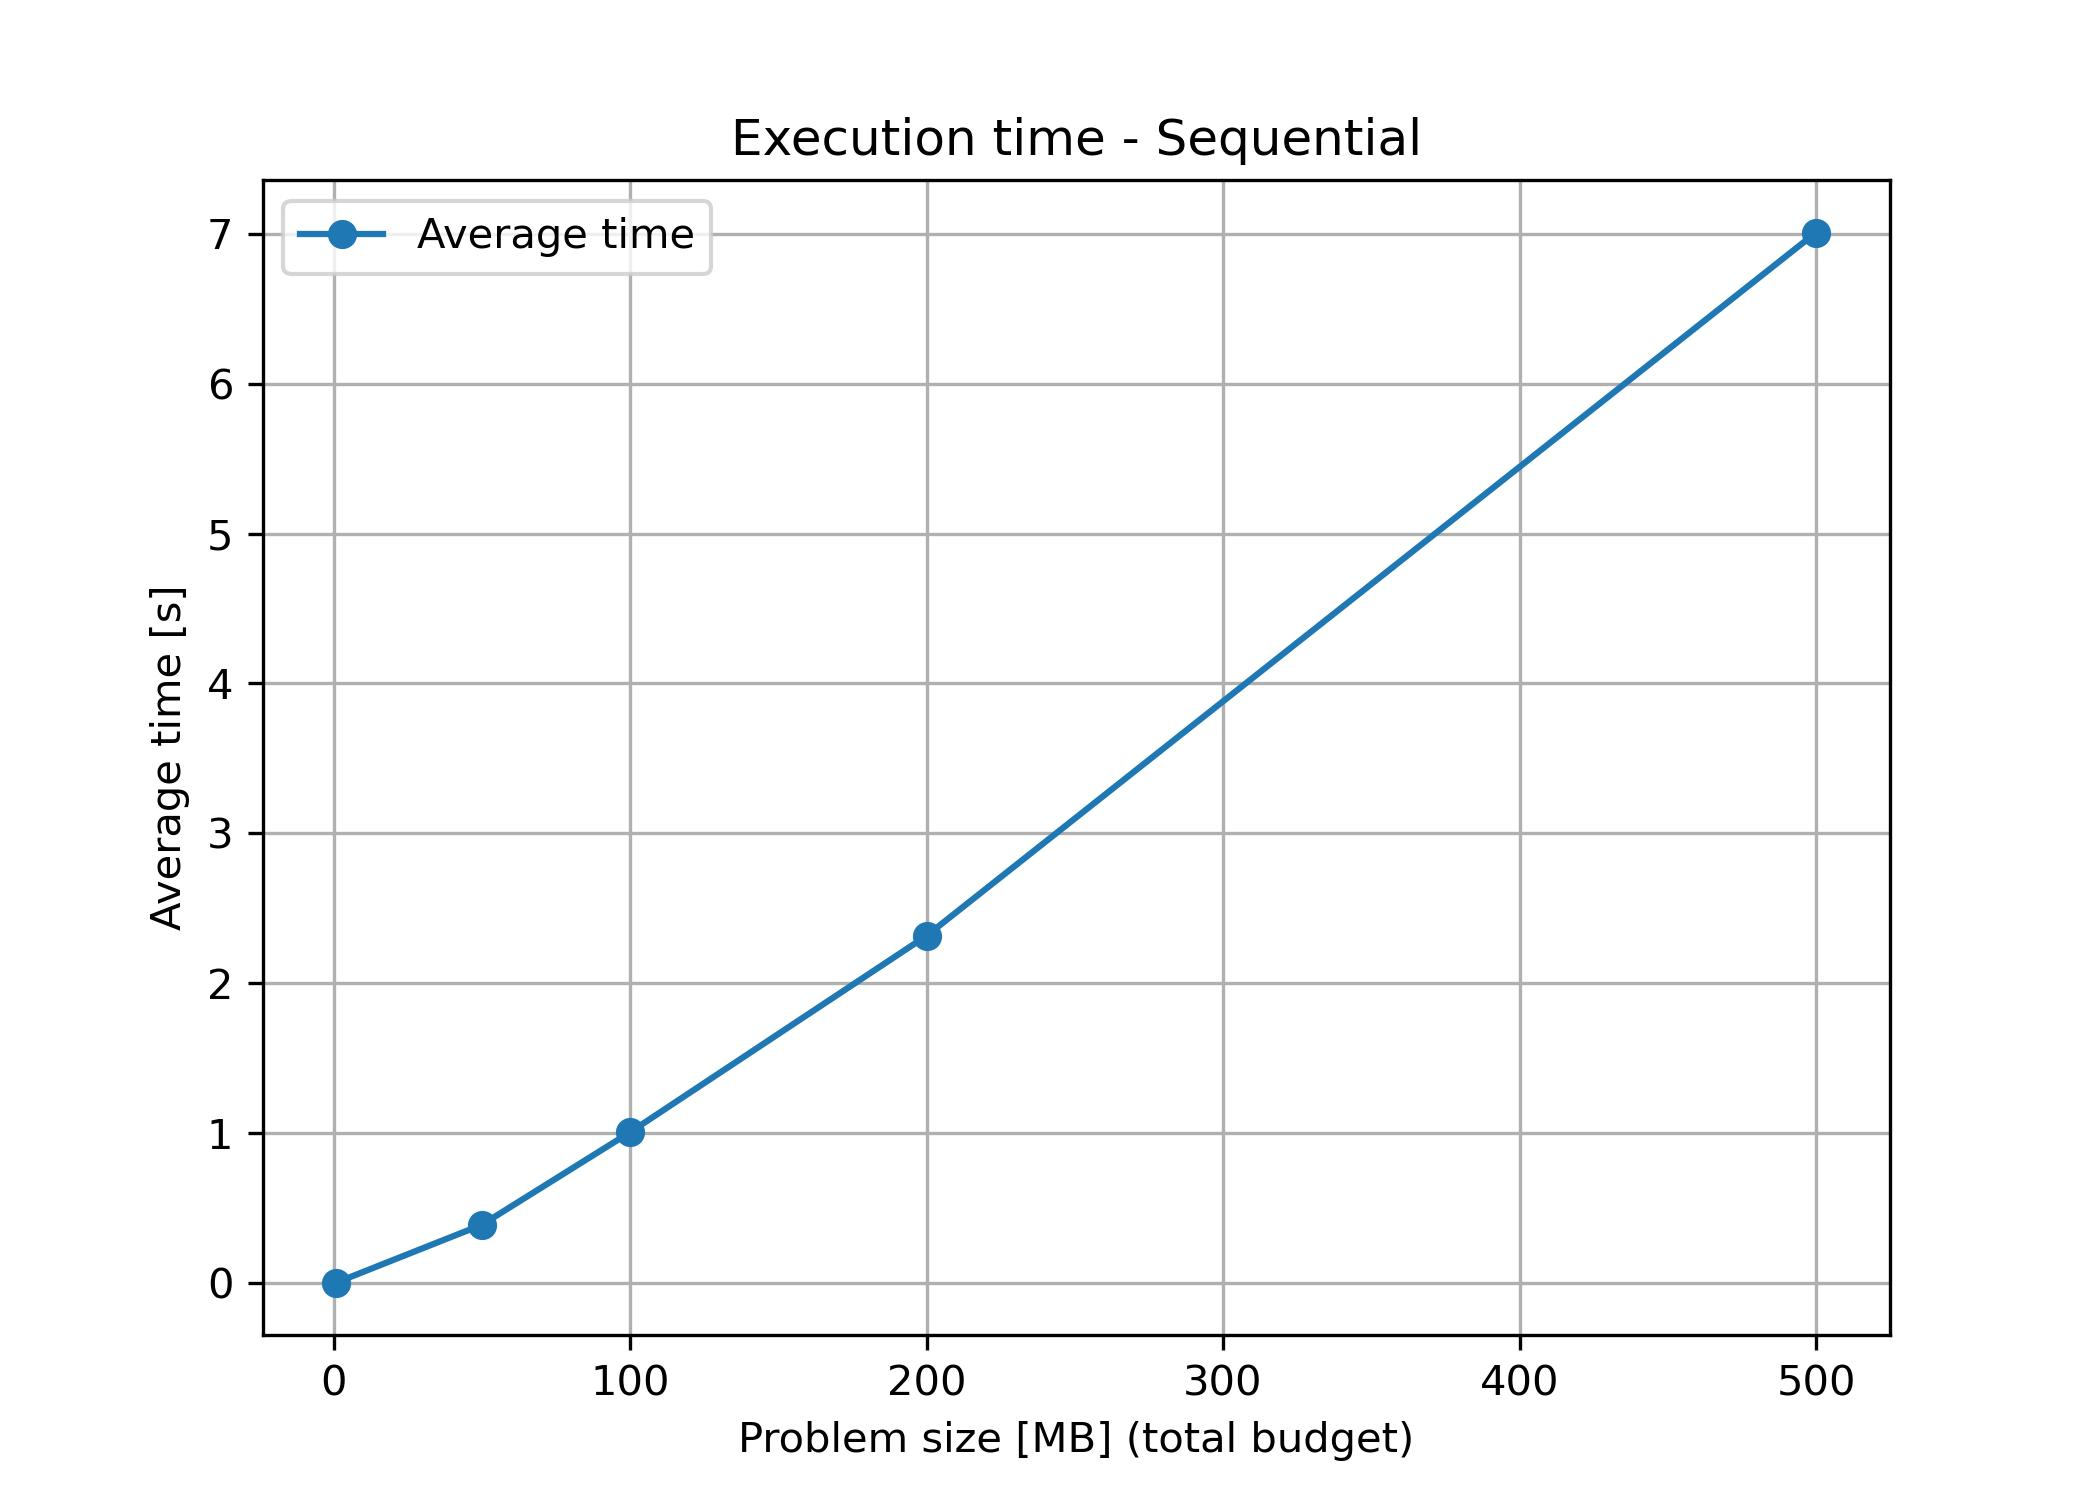
\includegraphics[width=1\linewidth]{img/seq_plots/seq_time.jpg}
				\caption{Tempi sequenziale}
				\label{fig:seq_time}
			\end{figure}
			
			\begin{figure}[H]
				\centering
				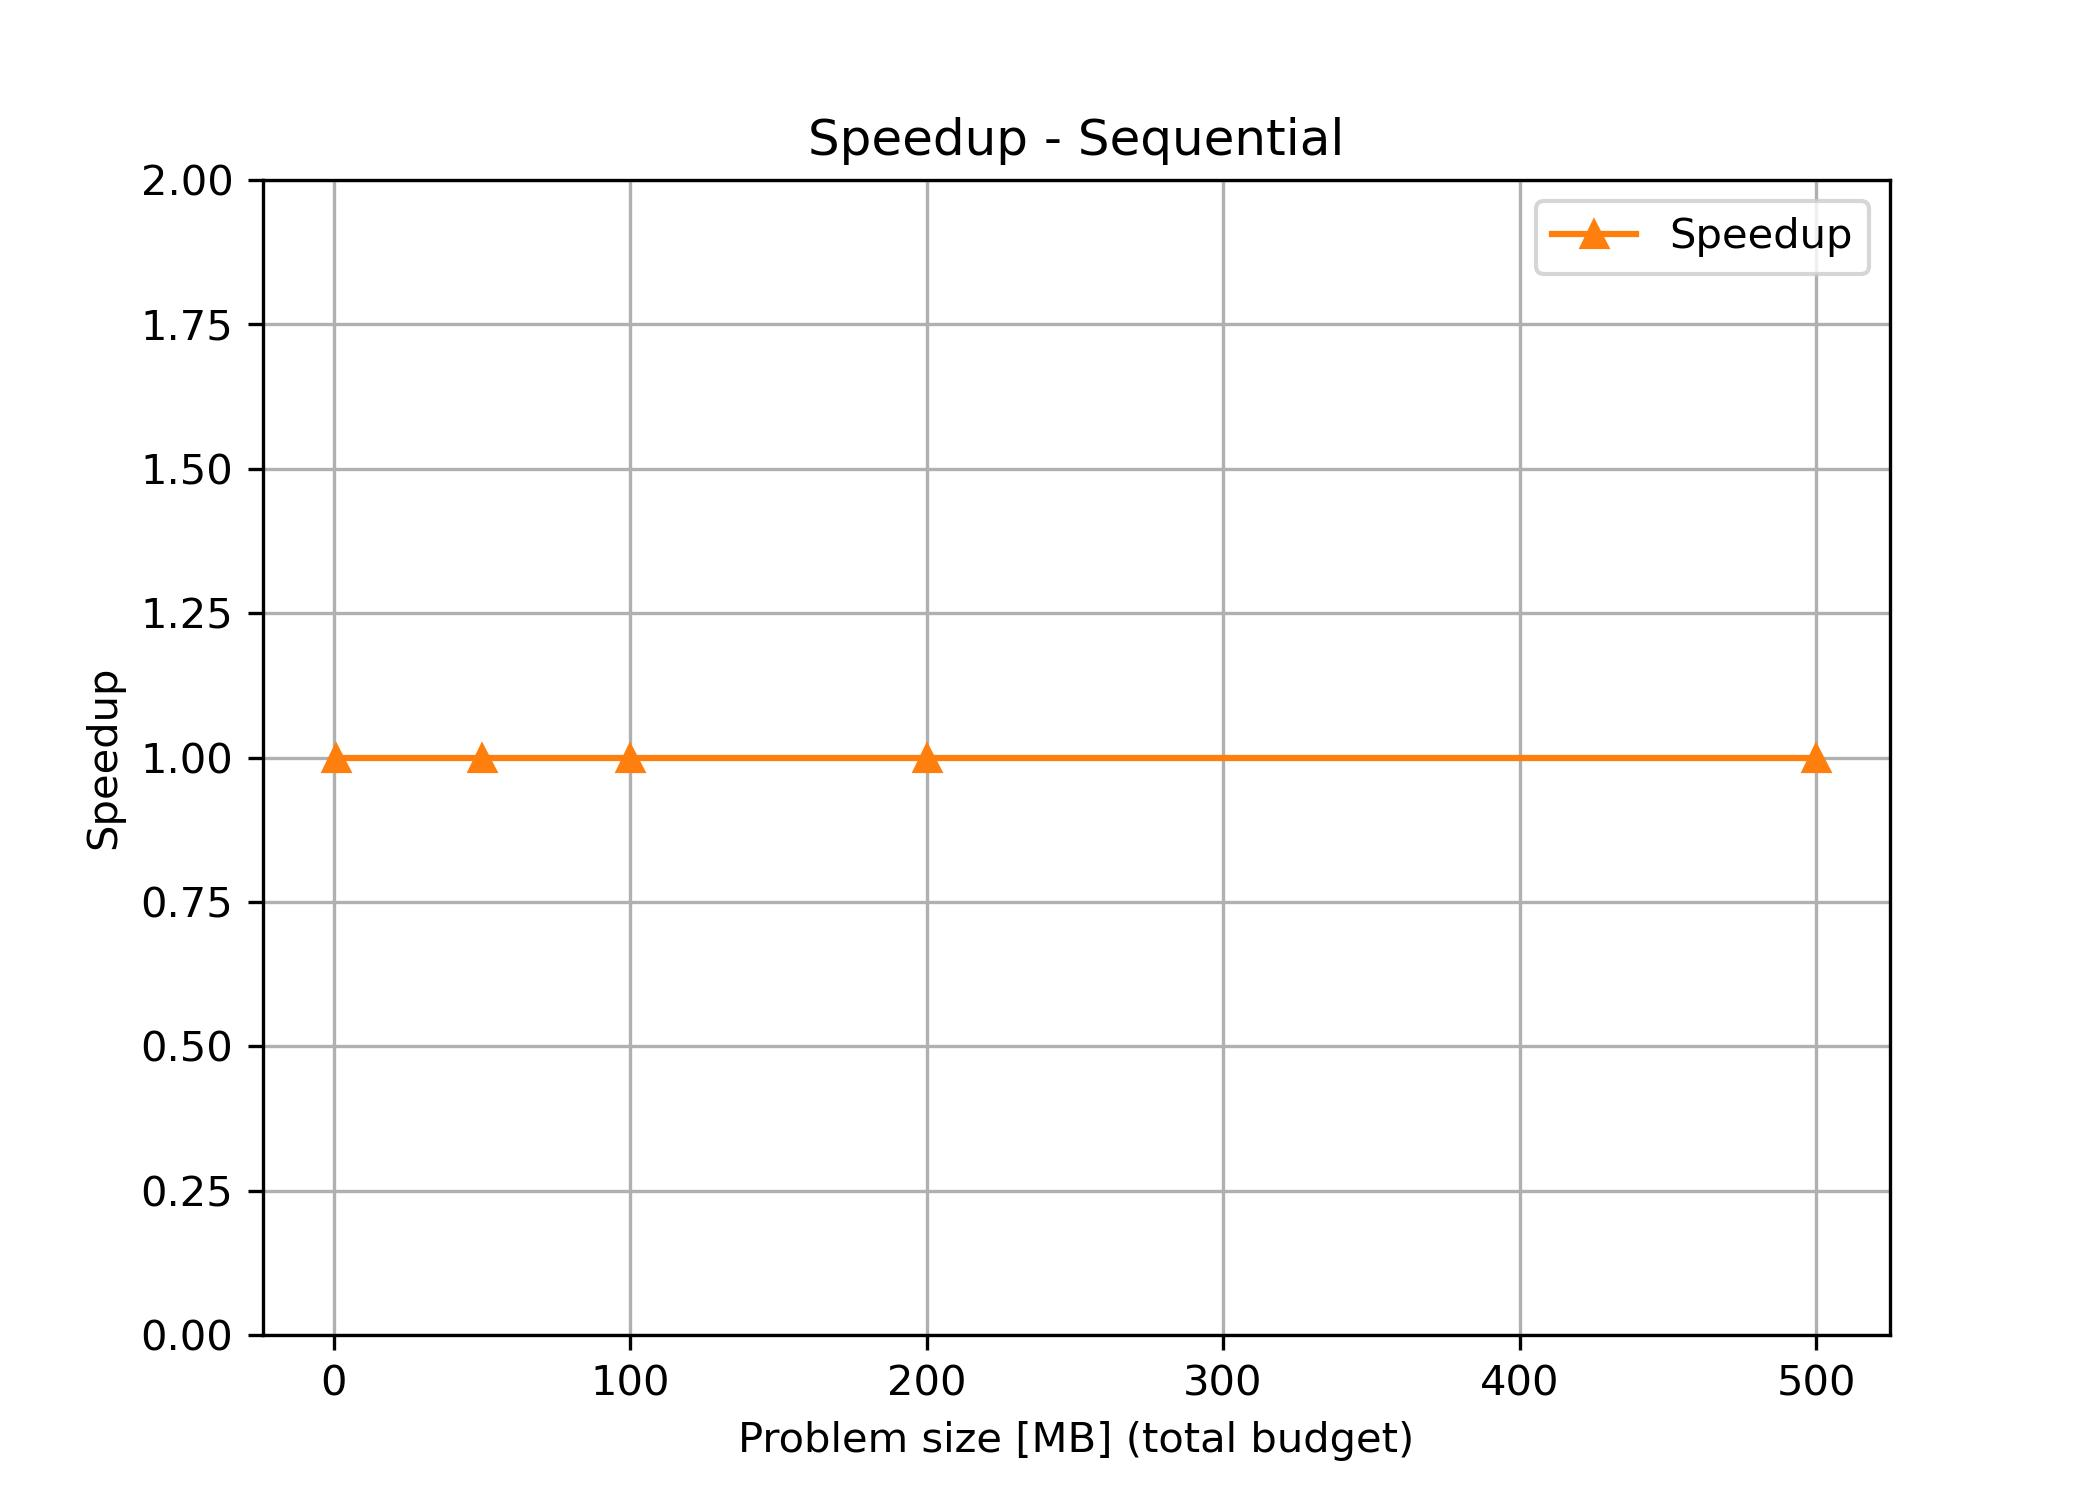
\includegraphics[width=1\linewidth]{img/seq_plots/seq_speedup.jpg}
				\caption{Speedup sequenziale}
				\label{fig:seq_speedup}
			\end{figure}
			
			\begin{figure}[H]
				\centering
				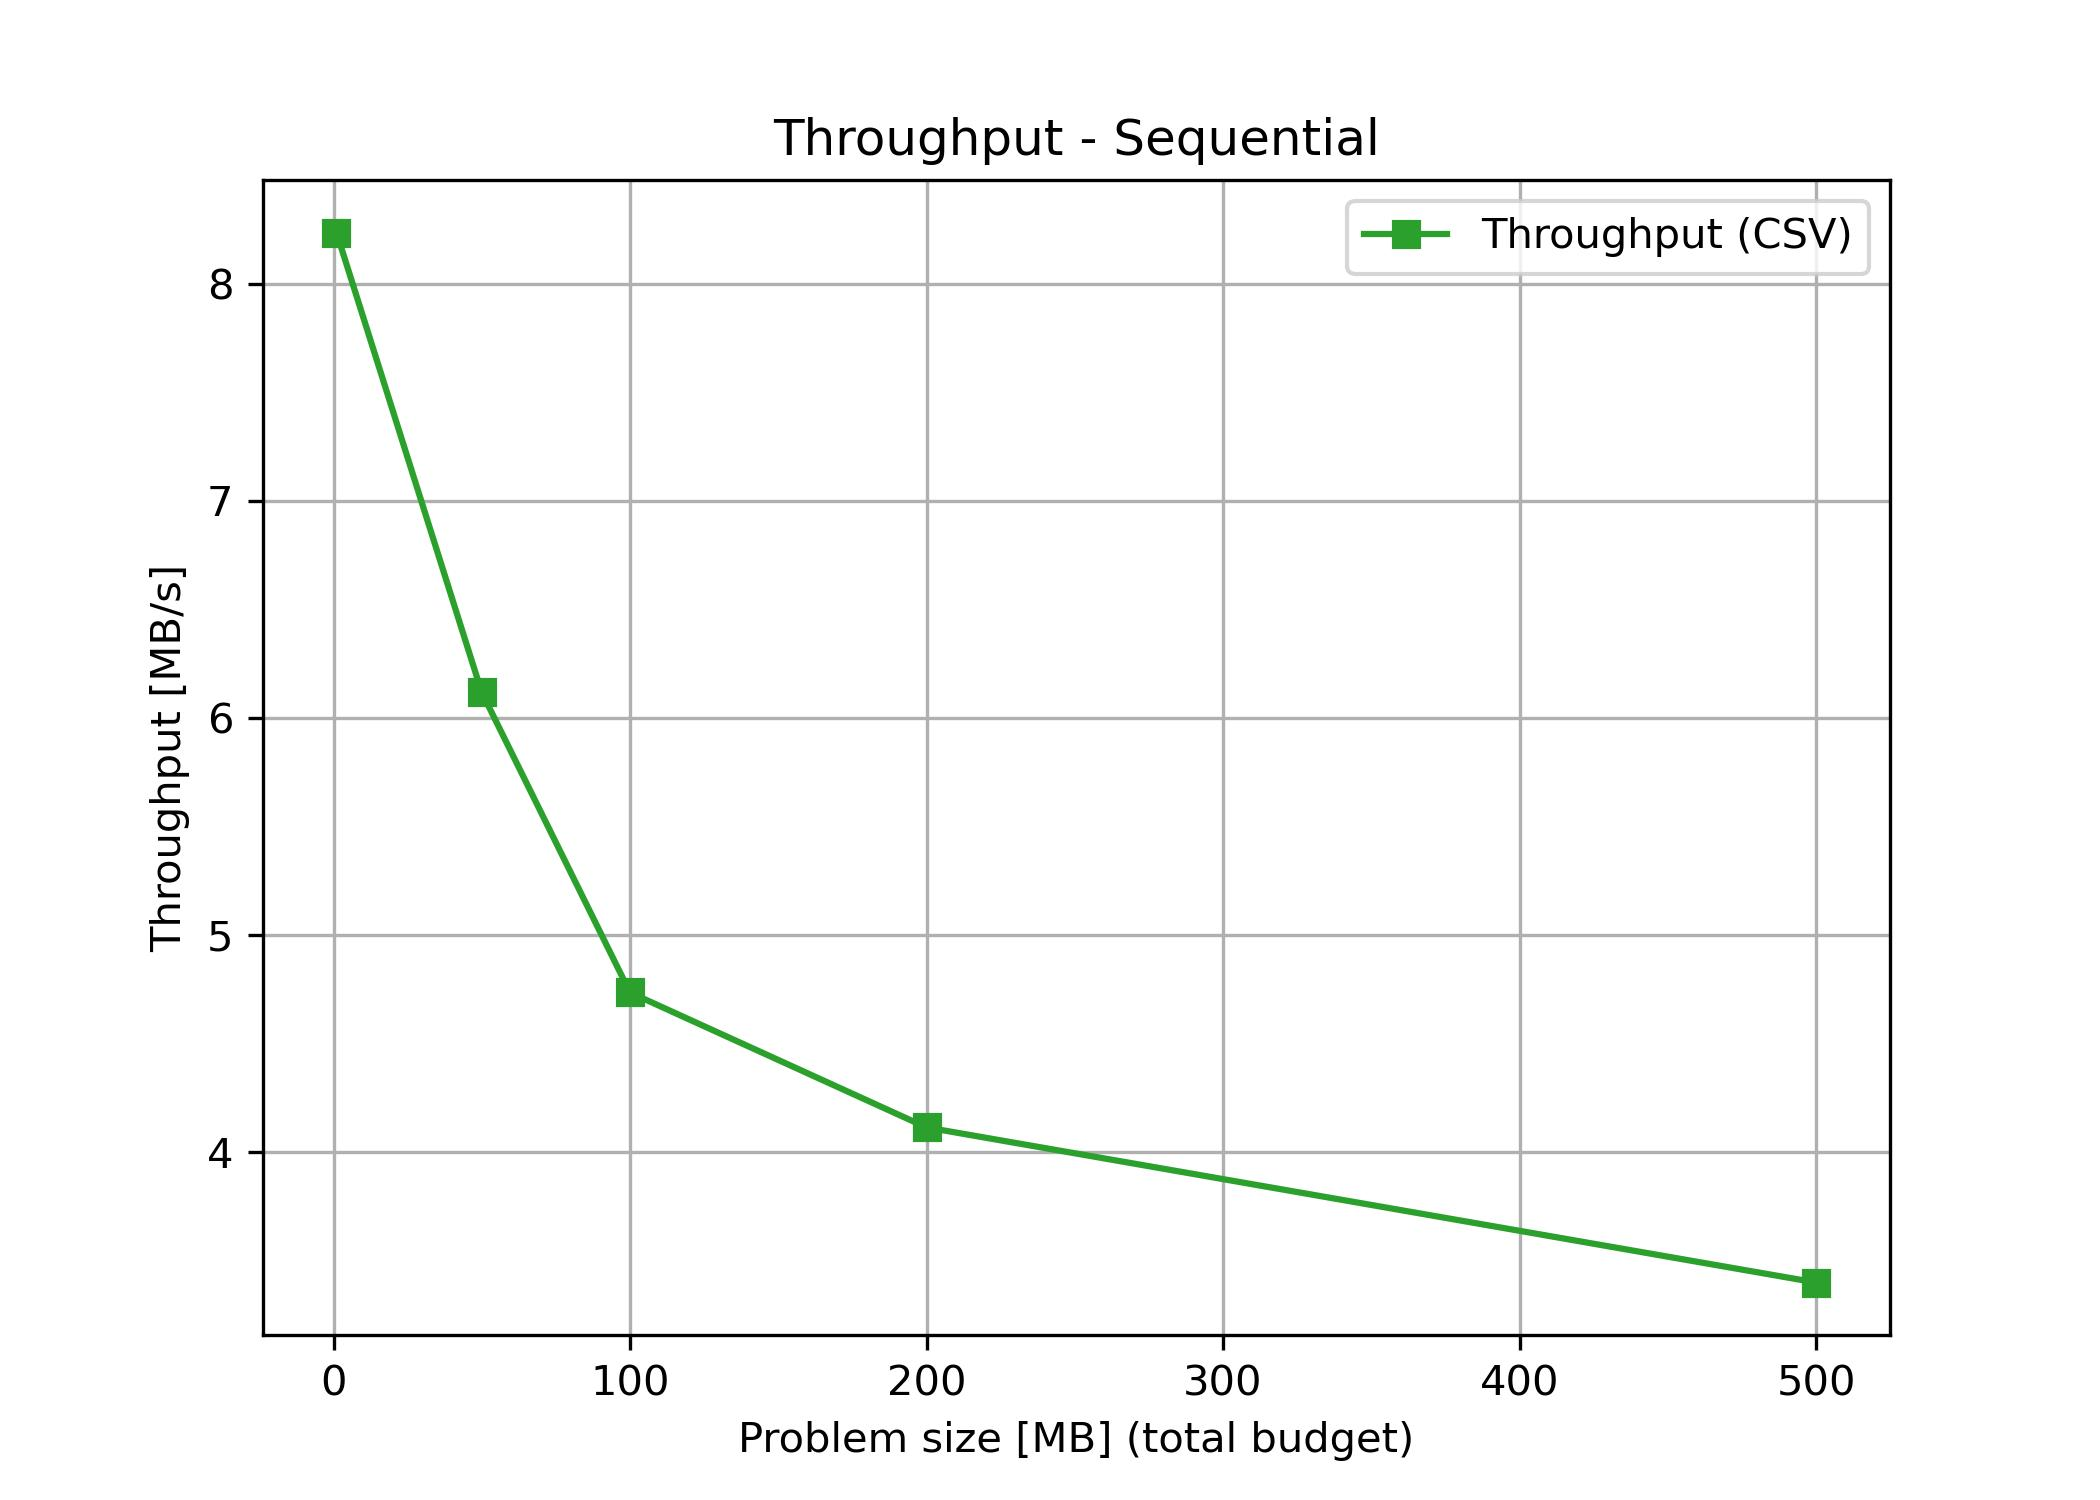
\includegraphics[width=1\linewidth]{img/seq_plots/seq_throughput.jpg}
				\caption{Throughput sequenziale}
				\label{fig:seq_throughput}
			\end{figure}
			
			\subsubsection*{Osservazioni}
				\begin{itemize}
						\item Il throughput decresce con la dimensione dell’input: da \(\sim 8.2\) MB/s (1 MB) a \(\sim 3.4\) MB/s (500 MB).
						\item La riduzione è coerente con la complessità \(O(n \log n)\) della costruzione SA, difatti all’aumentare di \(n\), il fattore logaritmico abbassa l’efficienza media.
						\item Per dataset piccoli, gli overhead fissi (\texttt{I/O}, allocazioni) pesano di più, causando un throughput apparente più elevato.
						\item La variabilità tra run è trascurabile ($<1$\% sui dataset grandi).
				\end{itemize}
		
		\subsection{Profiling della memoria}
			Il profiling della memoria è stato effettuato con \texttt{valgrind --tool=massif} sul dataset da 500 MB, producendo il file \texttt{seq\_500MB\_mem\_profile.txt}.
			Lo snapshot di picco riporta un consumo massimo di \(\sim 530\) MB, così suddivisi:
			\begin{enumerate}
				\item \(\sim 499\) MB (\(\sim 94\%\)) per i vettori \texttt{int} principali (\texttt{sa}, \texttt{rank}, \texttt{cnt}, \texttt{next}, \texttt{lcp});
				\item \(\sim 25\) MB (\(\sim 4.7\%\)) per il buffer \texttt{text};
				\item \(\sim 6.2\) MB (\(\sim 1.2\%\)) per i vettori booleani \texttt{bh}/\texttt{b2h}.
			\end{enumerate}
			
			\begin{figure}[H]
				\centering
				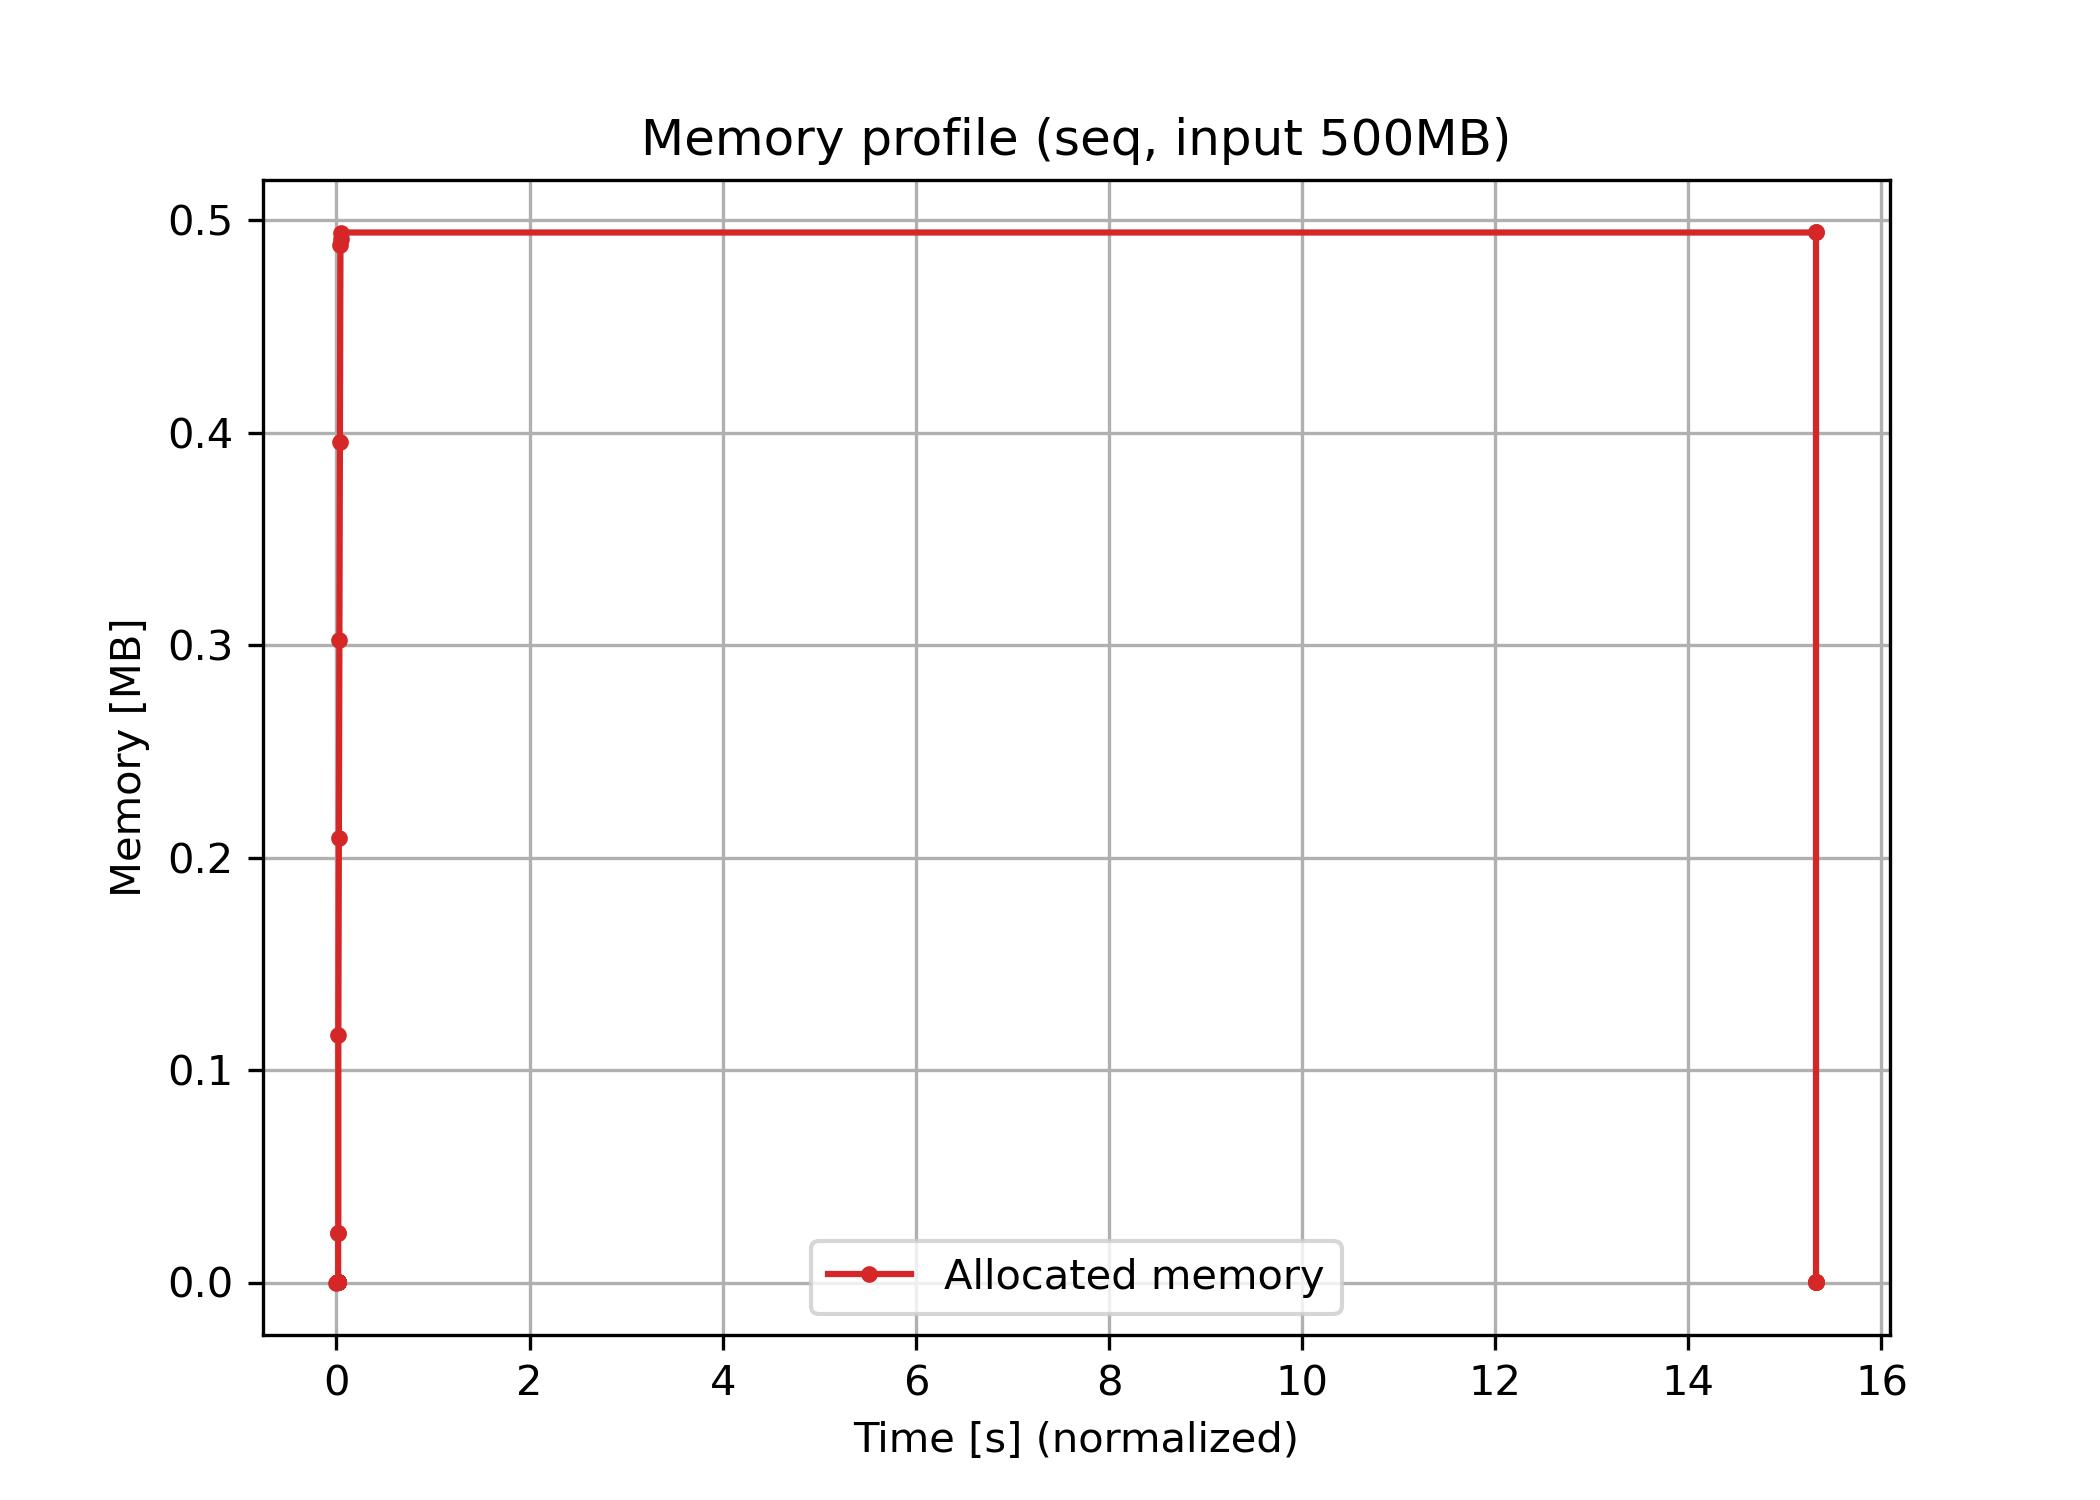
\includegraphics[width=1\linewidth]{img/seq_plots/seq_memory_profile.jpg}
				\caption{Memory usage sequenziale}
				\label{fig:seq_mem_usage}
			\end{figure}
			
			\subsubsection*{Confronto con l’analisi teorica}
				Nel WP1 era stato stimato un fabbisogno \(\approx 20n\) byte per i vettori di interi, più \(n\) byte per \texttt{text} e \(\frac{n}{4}\) byte per i vettori booleani.
				Per \(n=500\) MB il totale teorico atteso è \(\sim 530\) MB, perfettamente coerente con il picco misurato di \(\sim 530.6\) MB.
			
			\subsubsection*{Conclusione}
				La versione sequenziale evidenzia quindi un comportamento sia temporale che spaziale pienamente conforme all’analisi asintotica:
				prestazioni scalabili con \(n \log n\) e footprint di memoria dominato dai vettori ausiliari.
	
	\section{Versione OpenMP}
		
		\subsection{Analisi dei tempi}
			Le prestazioni sono state valutate con 2, 4 e 8 thread.
			I risultati medi su 10 run, ottenuti dai file \texttt{omp\_summary\_2.csv}, \texttt{omp\_summary\_4.csv} e \texttt{omp\_summary\_8.csv}, sono riportati nella Tabella~\ref{tab:omp-summary}.
			
			\begin{table}[H]
				\centering
				\begin{tabular}{|r|r|r|r|r|}
					\hline
					\textbf{Threads} & \textbf{Dimensione} & \textbf{Tempo medio [s]} & \textbf{Speedup} & \textbf{Efficienza [\%]} \\
					\hline
					2                     & 1 MB                & 0.0058                   & 1.12             & 56.2                     \\
					2                     & 50 MB               & 0.436                    & 0.95             & 47.7                     \\
					2                     & 100 MB              & 1.079                    & 0.98             & 48.8                     \\
					2                     & 200 MB              & 2.600                    & 0.92             & 46.1                     \\
					2                     & 500 MB              & 7.476                    & 0.96             & 48.2                     \\
					\hline
					4                     & 1 MB                & 0.0063                   & 1.02             & 25.5                     \\
					4                     & 50 MB               & 0.390                    & 1.07             & 26.7                     \\
					4                     & 100 MB              & 1.010                    & 1.04             & 26.0                     \\
					4                     & 200 MB              & 2.517                    & 0.95             & 23.8                     \\
					4                     & 500 MB              & 7.119                    & 1.01             & 25.3                     \\
					\hline
					8                     & 1 MB                & 0.0064                   & 1.02             & 12.7                     \\
					8                     & 50 MB               & 0.392                    & 1.06             & 13.3                     \\
					8                     & 100 MB              & 1.023                    & 1.03             & 12.9                     \\
					8                     & 200 MB              & 2.475                    & 0.97             & 12.1                     \\
					8                     & 500 MB              & 7.245                    & 1.00             & 12.4                     \\
					\hline
				\end{tabular}
				\caption{Risultati OpenMP (medie su 10 run): tempi, speedup ed efficienza.}
				\label{tab:omp-summary}
			\end{table}
			
			\begin{figure}[H]
				\centering
				\begin{minipage}[t]{0.49\textwidth}
					\centering
					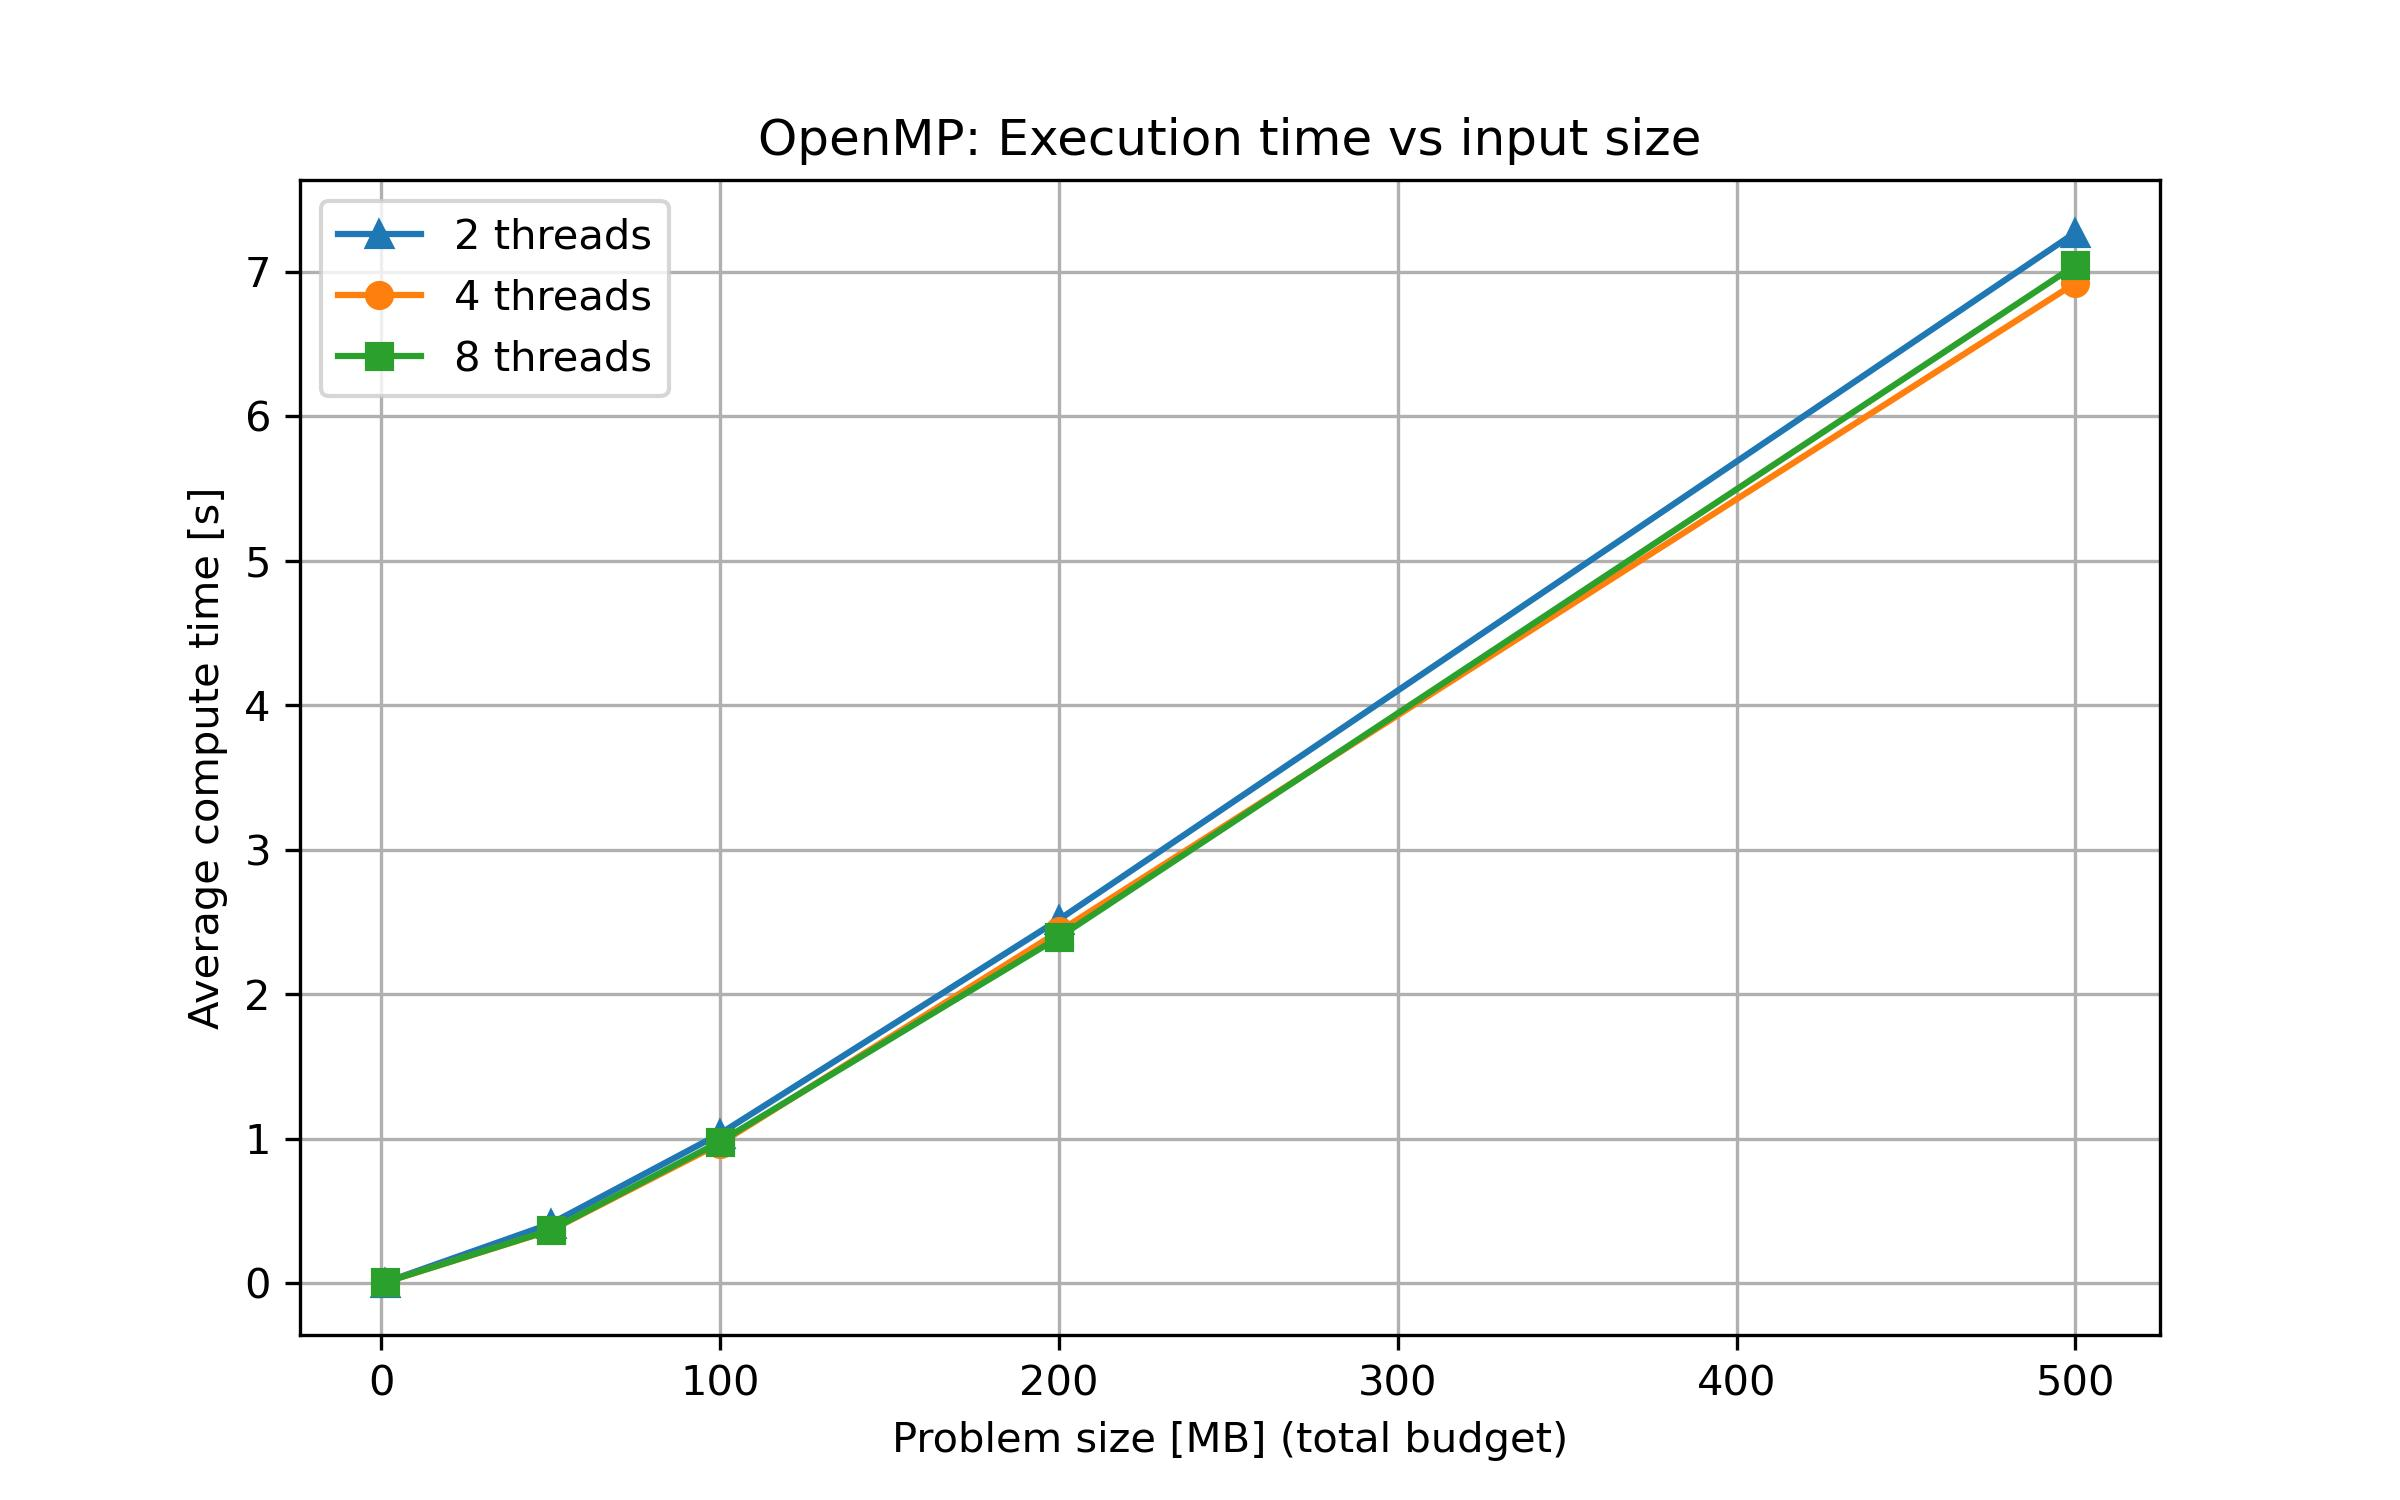
\includegraphics[width=\textwidth]{img/omp_plots/omp_times.jpg}
					\caption{Tempi OpenMP}
					\label{fig:omp_times}
				\end{minipage}
				\hfill
				\begin{minipage}[t]{0.49\textwidth}
					\centering
					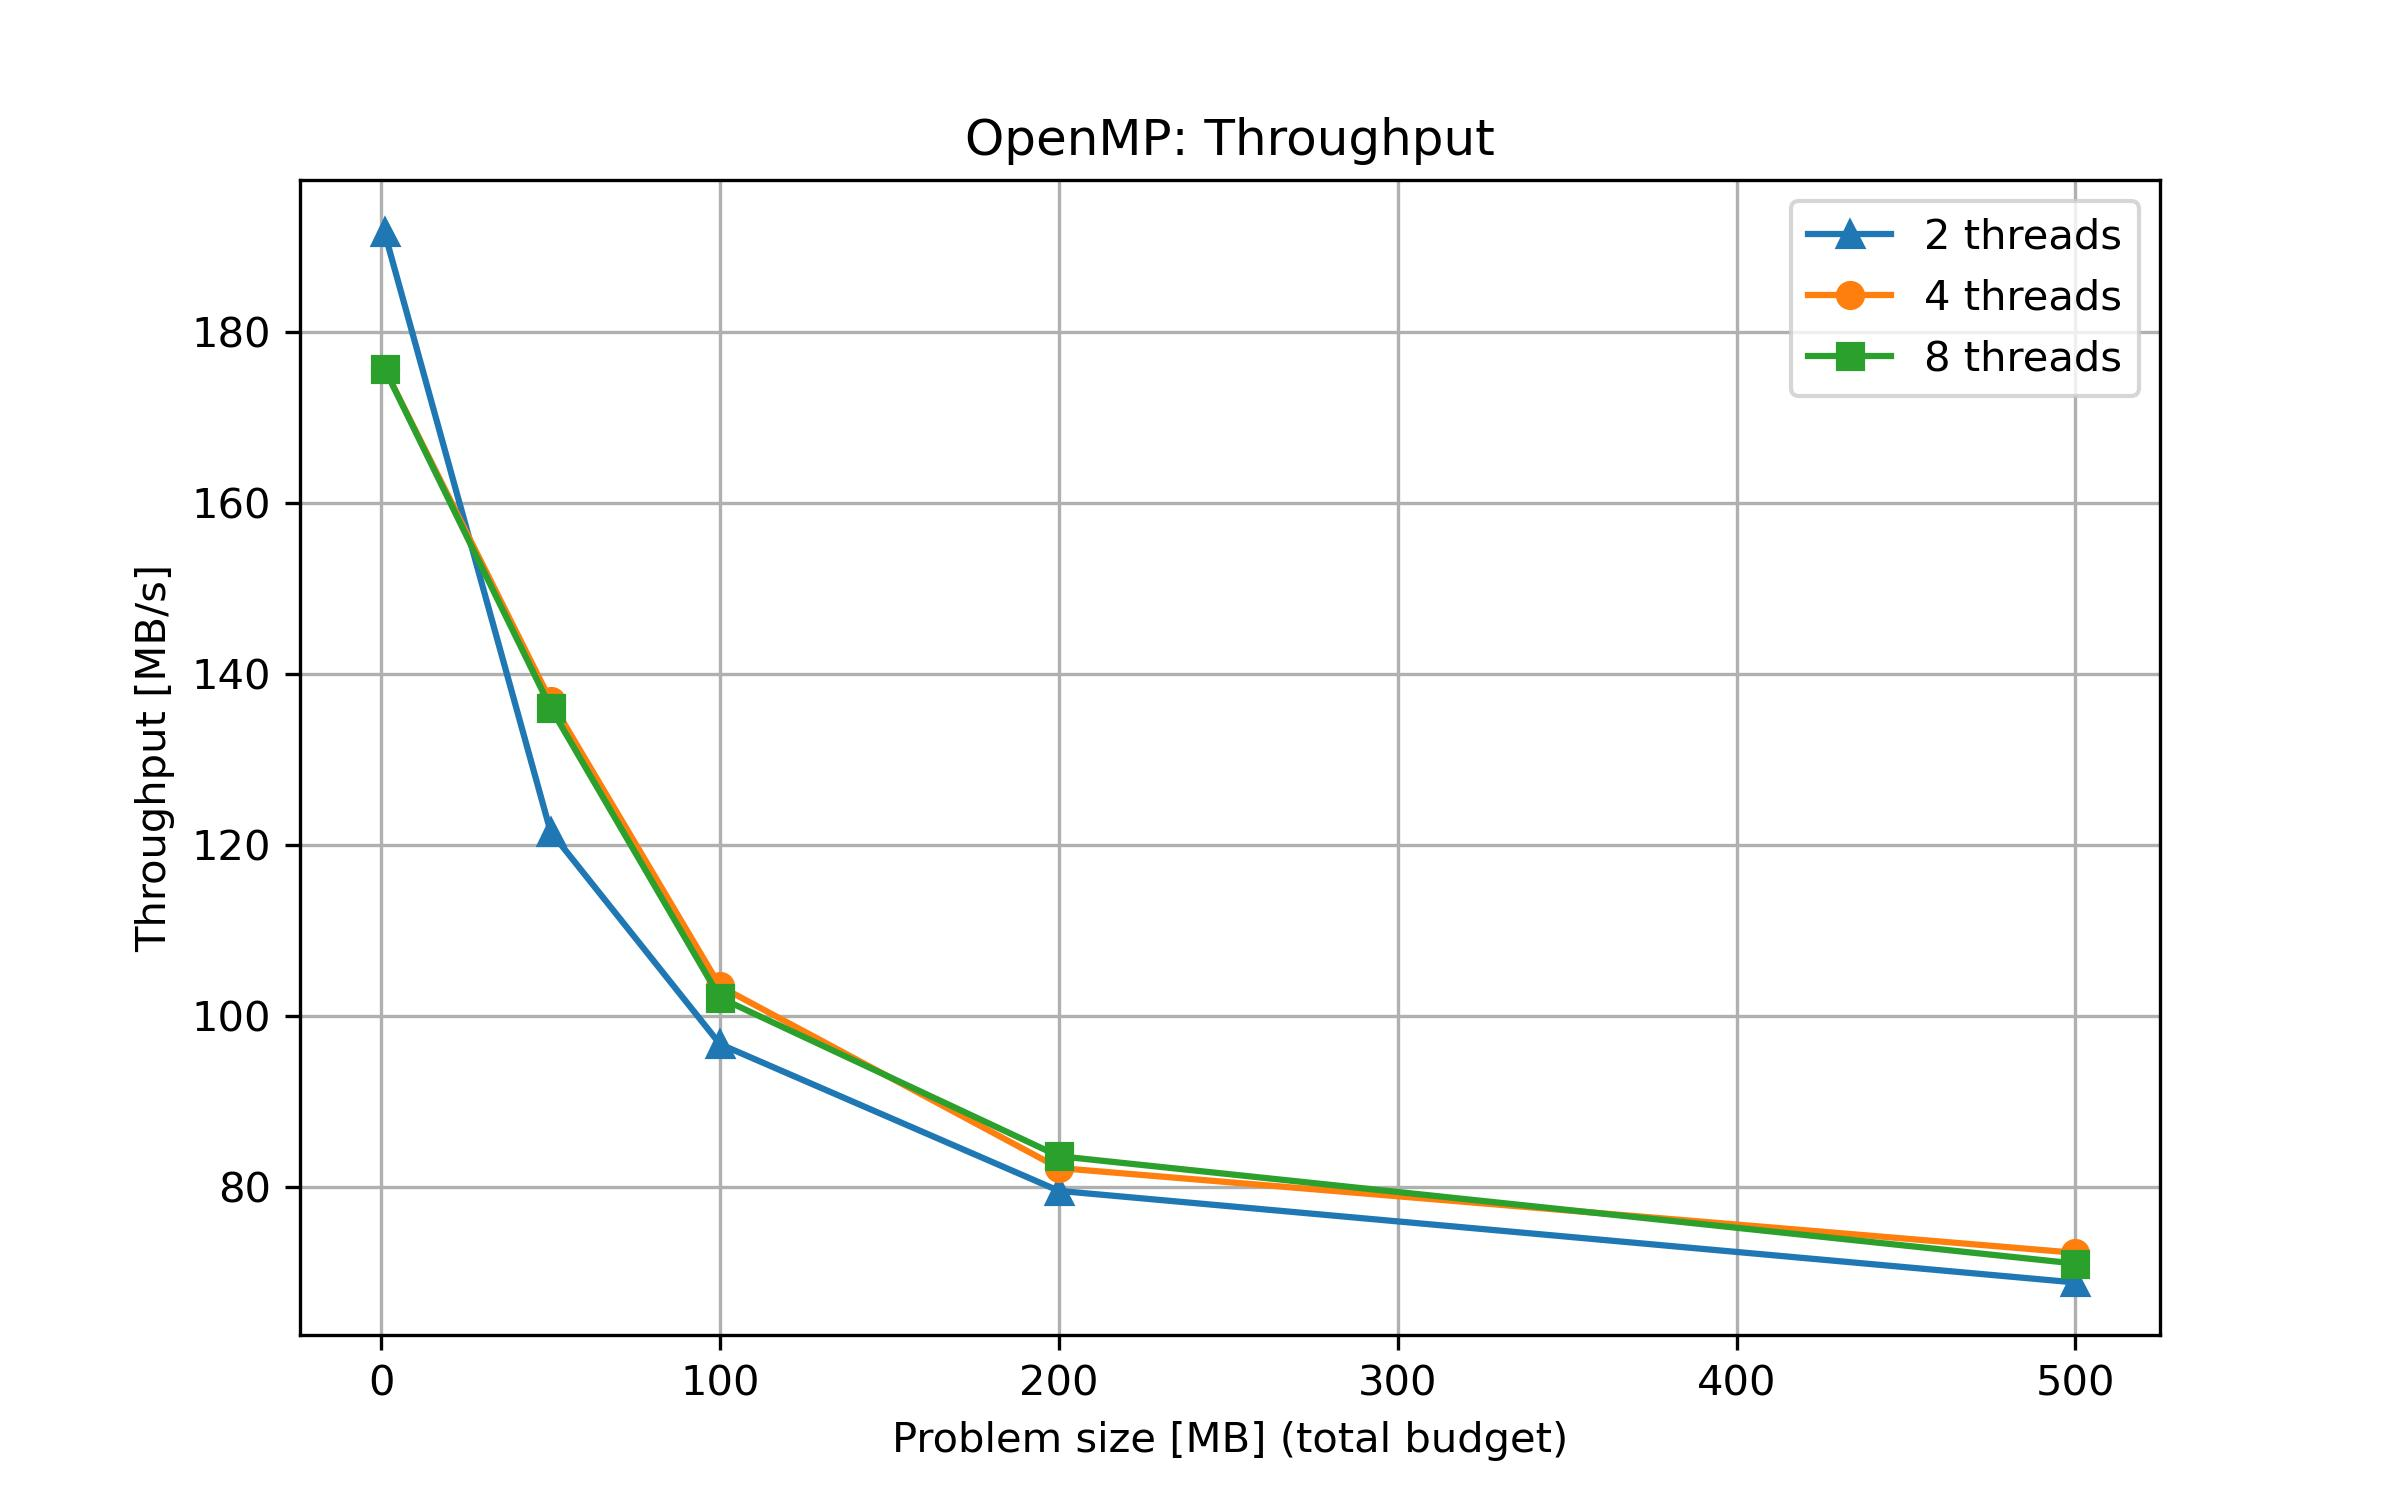
\includegraphics[width=\textwidth]{img/omp_plots/omp_throughput.jpg}
					\caption{Throughput OpenMP}
					\label{fig:omp_throughput}
				\end{minipage}
			\end{figure}
			
			\begin{figure}[H]
				\centering
				\begin{minipage}[t]{0.49\textwidth}
					\centering
					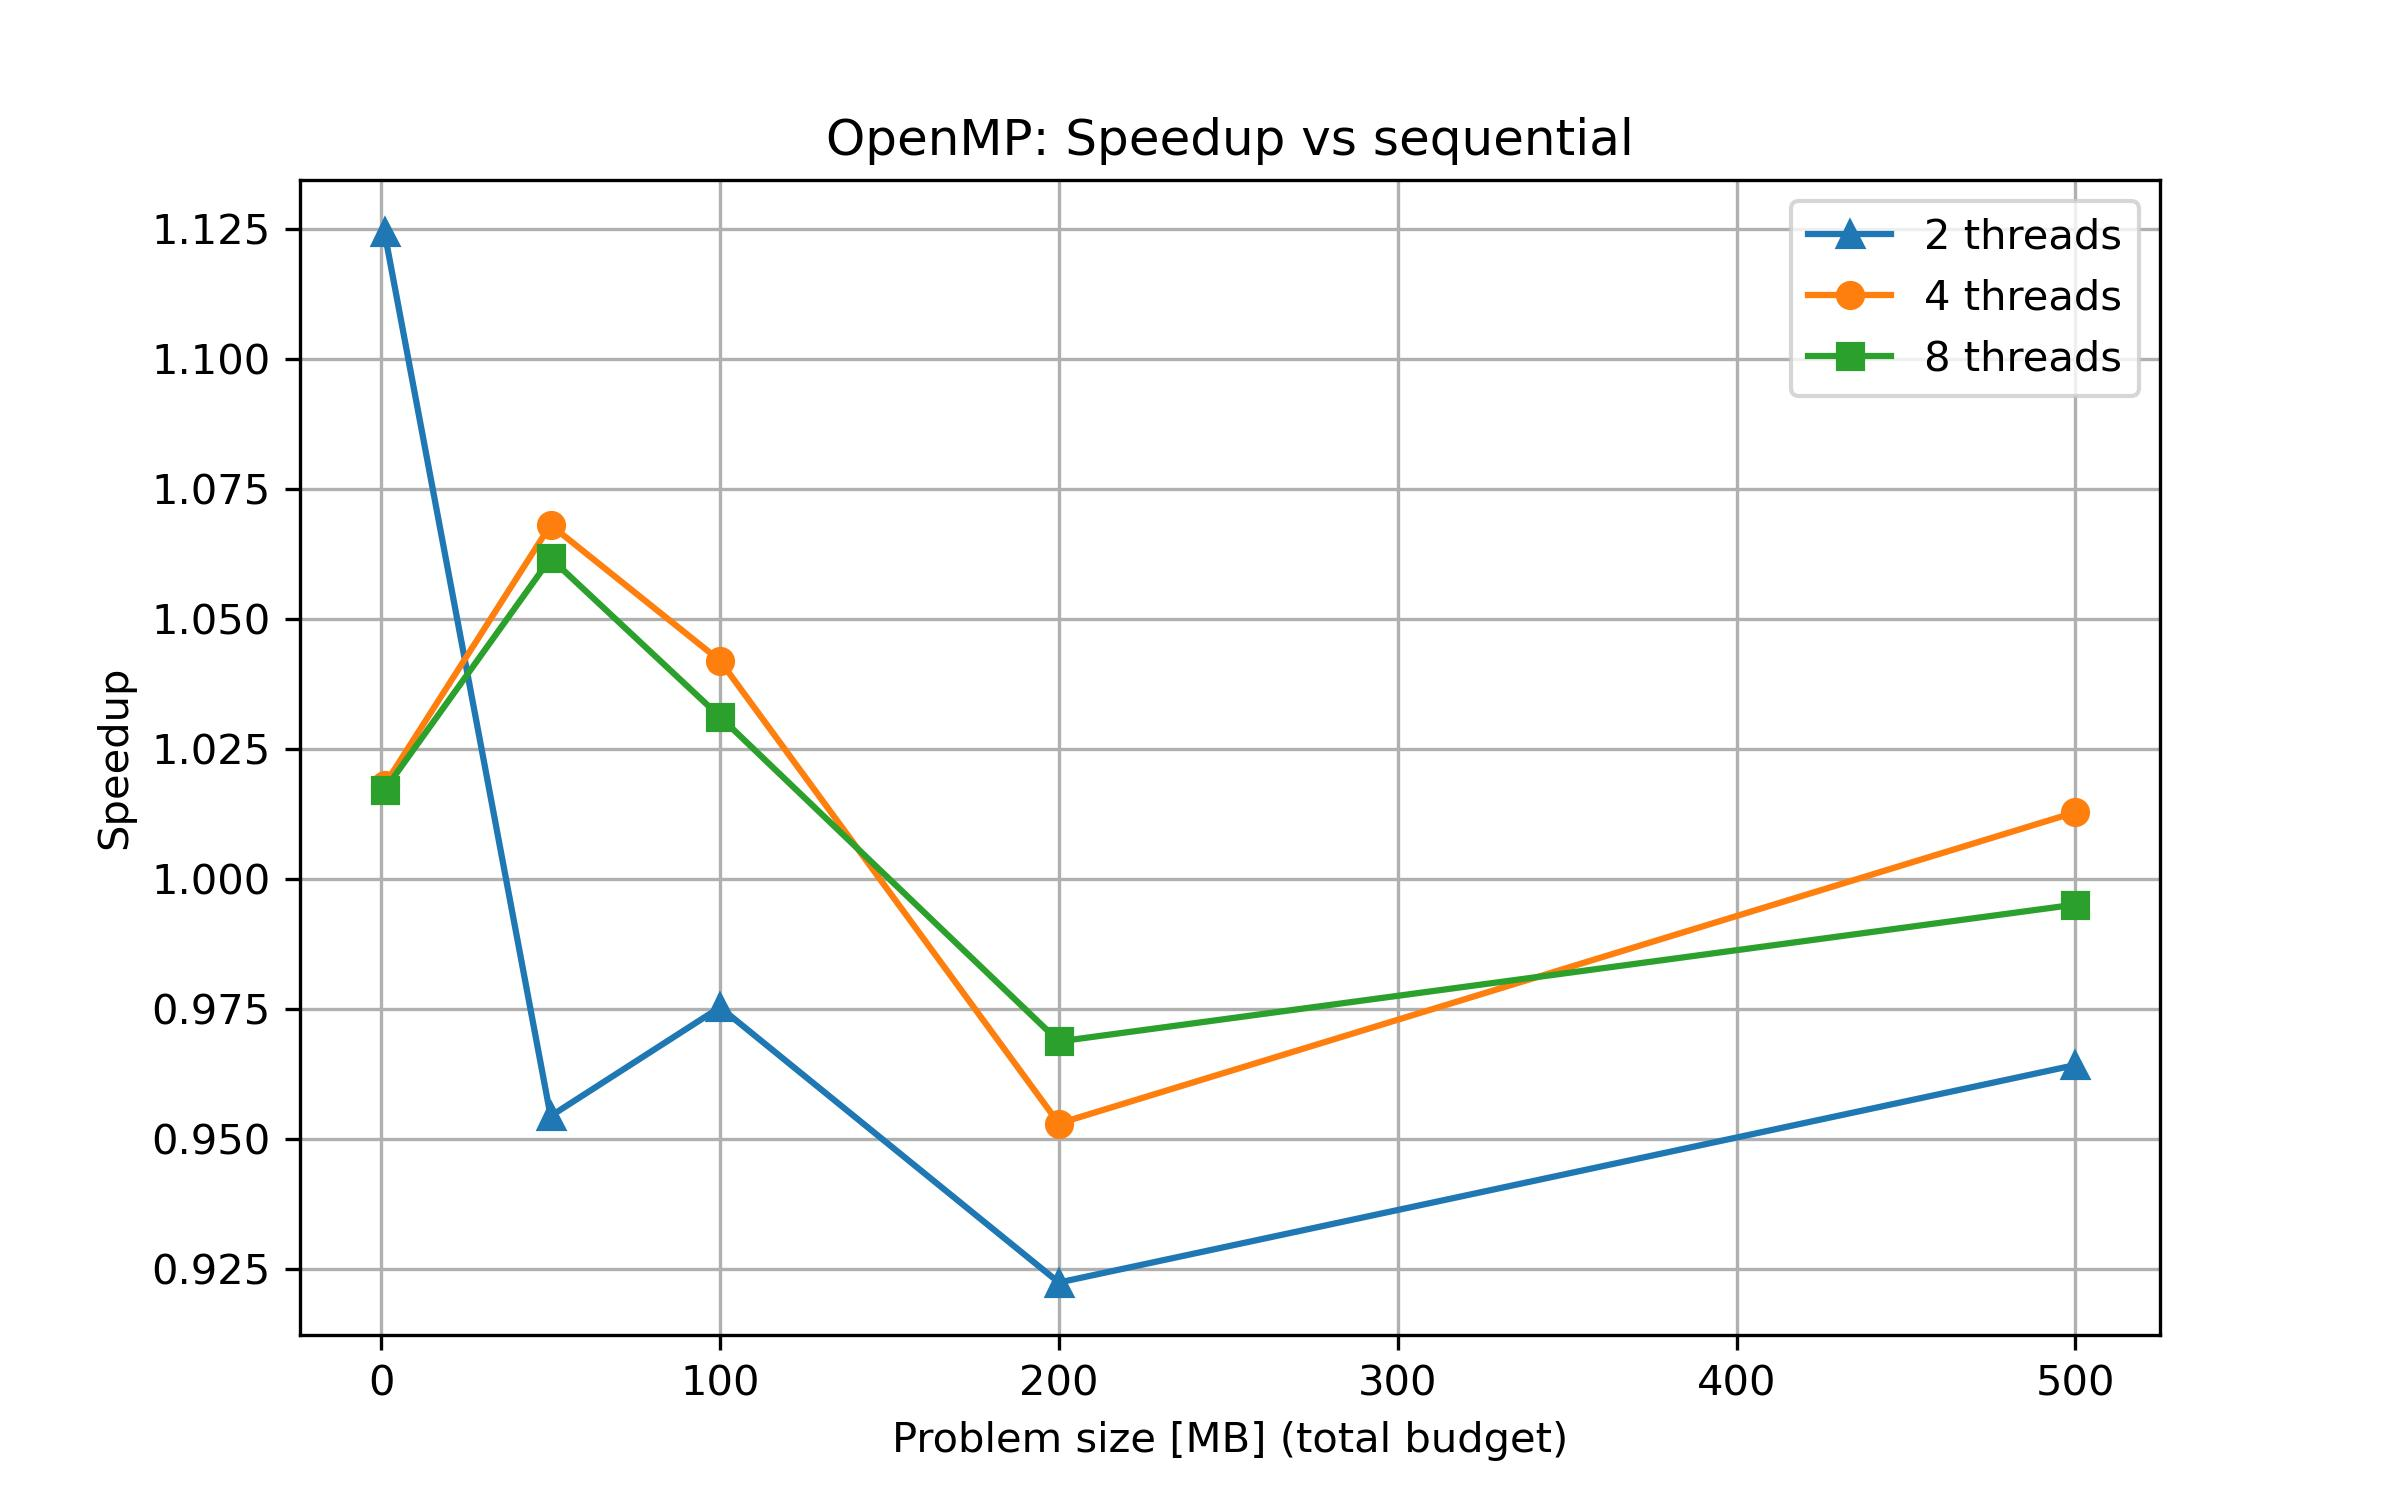
\includegraphics[width=\textwidth]{img/omp_plots/omp_speedup.jpg}
					\caption{Speedup OpenMP}
					\label{fig:omp_speedup}
				\end{minipage}
				\hfill
				\begin{minipage}[t]{0.49\textwidth}
					\centering
					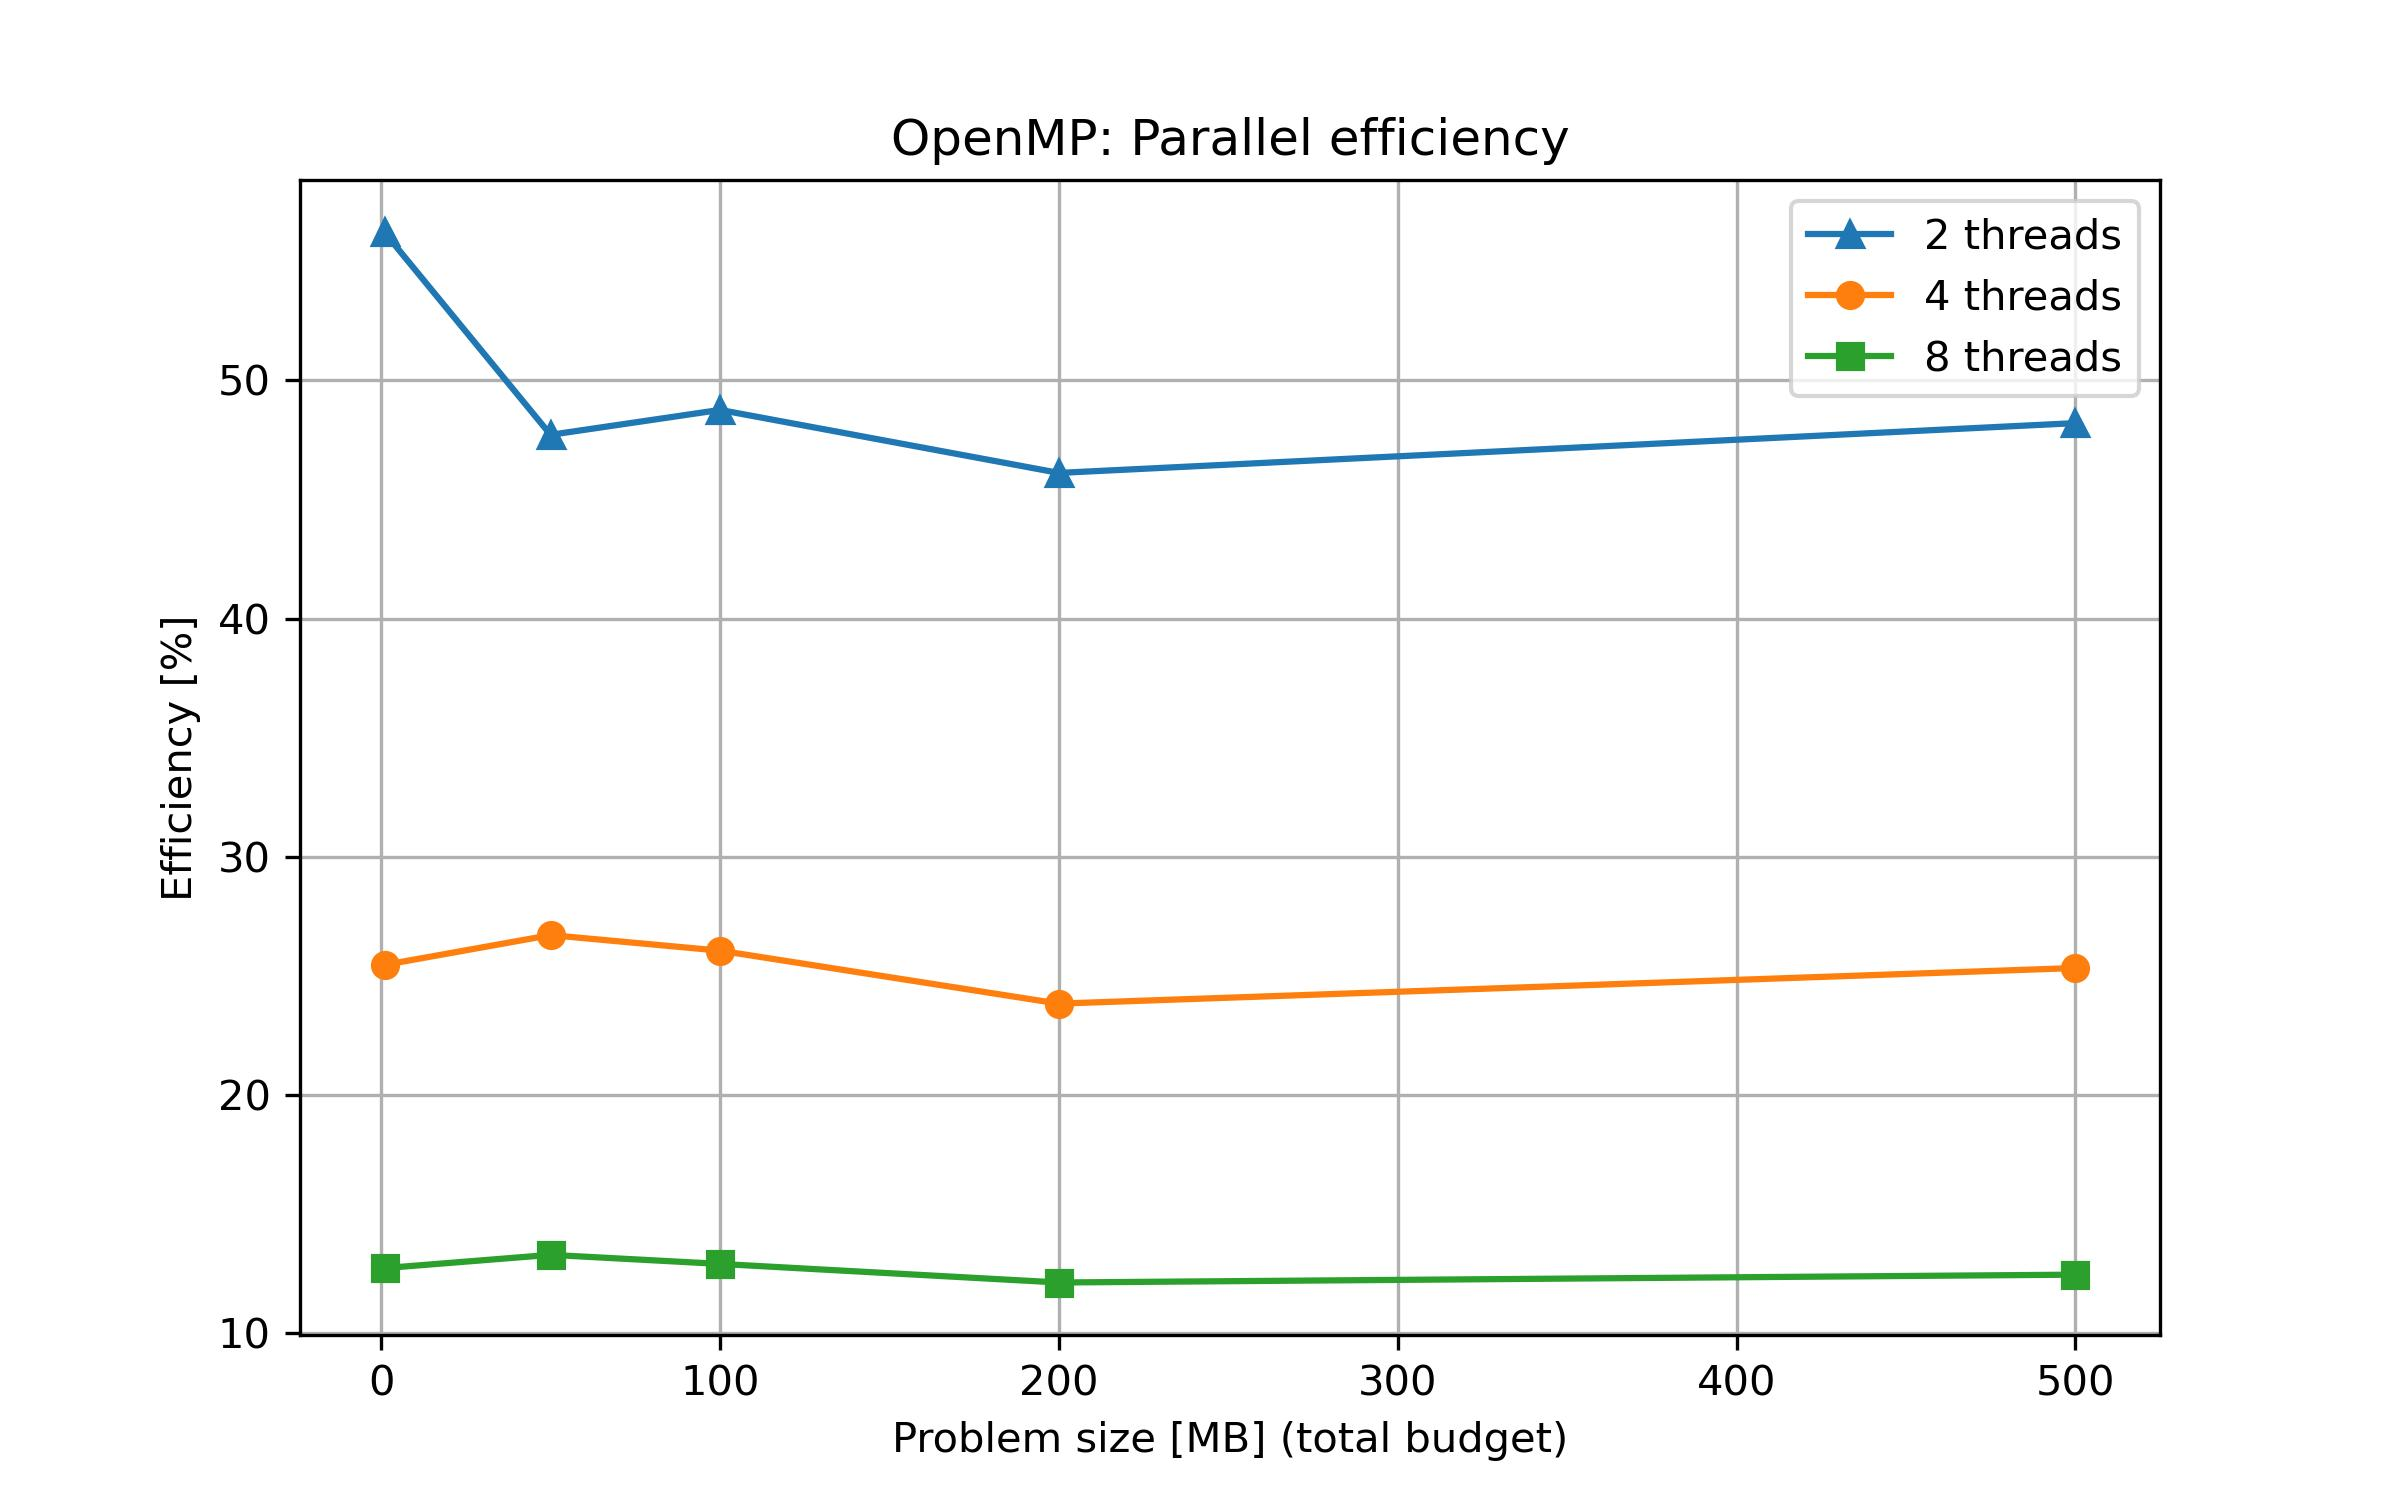
\includegraphics[width=\textwidth]{img/omp_plots/omp_efficiency.jpg}
					\caption{Efficiency OpenMP}
					\label{fig:omp_efficiency}
				\end{minipage}
			\end{figure}
			
			\subsubsection*{Osservazioni}
				\begin{itemize}
						\item Con 2 thread si osserva in media un lieve degrado rispetto al sequenziale (speedup $\sim$0.95--0.98$\times$ su dataset grandi).
						\item Con 4 thread lo speedup raggiunge al massimo $\sim$1.07$\times$, con efficienza intorno al 25\%.
						\item Con 8 thread le prestazioni non migliorano ulteriormente: lo speedup resta $\sim$1.0--1.03$\times$ e l’efficienza scende sotto il 13\%.
						\item L’implementazione OpenMP mostra quindi un guadagno prestazionale molto limitato, penalizzato da colli di bottiglia di memoria e sezioni sequenziali non parallelizzate.
				\end{itemize}
		
		\subsection{Profiling della memoria}
			Il profiling con \texttt{valgrind --tool=massif} è stato eseguito su input da 500 MB (\texttt{seq\_omp\_2t\_500MB\_mem\_profile.txt}, \texttt{seq\_omp\_4t\_500MB\_mem\_profile.txt}, \texttt{seq\_omp\_8t\_500MB\_mem\_profile.txt}).
			In tutti i casi, il picco massimo si attesta intorno a \textbf{530 MB}, così suddivisi:
			\begin{itemize}
				\item $\sim$499 MB (94\%) per i vettori \texttt{int} principali (\texttt{sa}, \texttt{rank}, \texttt{cnt}, \texttt{next}, \texttt{lcp});
				\item $\sim$25 MB (4.7\%) per il buffer \texttt{text};
				\item $\sim$6 MB (1.2\%) per i vettori booleani \texttt{bh}/\texttt{b2h}.
			\end{itemize}
			
			\subsubsection*{Confronto 2 vs 4 vs 8 thread}
				\begin{itemize}
						\item I profili di memoria risultano praticamente identici: OpenMP non introduce copie ulteriori dei buffer, ma lavora sugli stessi dati condivisi.
						\item L’unica differenza rilevabile è un leggero incremento nello stack per i thread aggiuntivi, trascurabile rispetto al footprint complessivo.
				\end{itemize}
				
				\begin{figure}[H]
						\centering
						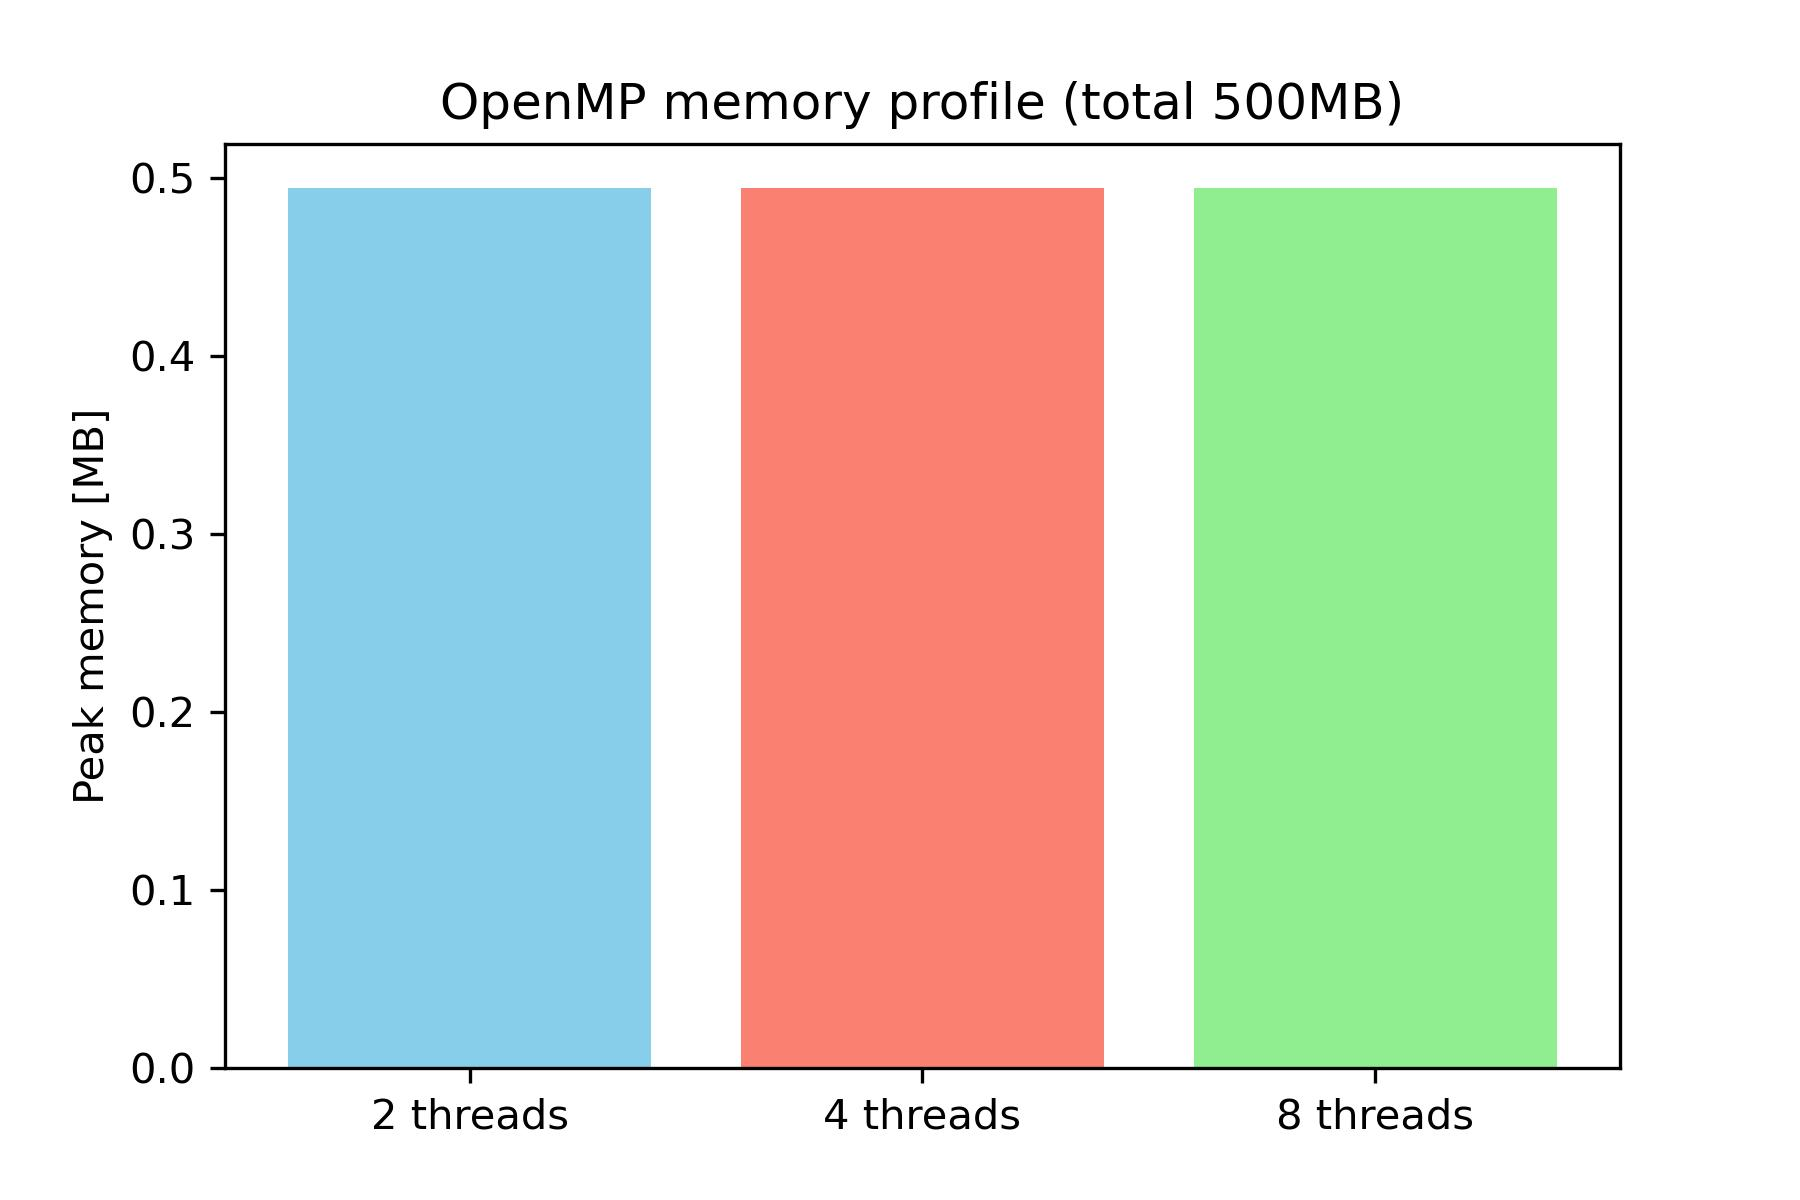
\includegraphics[width=1\linewidth]{img/omp_plots/omp_memory.jpg}
						\caption{Memory usage OpenMP (500 MB)}
						\label{fig:omp_mem_usage}
				\end{figure}
			
			\subsubsection*{Conclusione}
				L’uso di OpenMP non riduce il fabbisogno di memoria rispetto al sequenziale, mentre i benefici sui tempi sono molto contenuti.
				Lo speedup resta nell’intervallo $0.95\text{--}1.07\times$ con efficienza bassa, segno che la natura dell’algoritmo e l’accesso irregolare ai dati non si prestano bene alla parallelizzazione a memoria condivisa.
	
	\section{Versione MPI}
		
		\subsection{Analisi dei tempi}
			Le prestazioni della versione distribuita sono state valutate con 10 run per ciascun dataset
			\(\{1, 50, 100, 200, 500\}\,\)MB e per tre configurazioni di ranks (\(2,4,8\)).
			I risultati medi (\texttt{mpi\_summary\_2.csv}, \texttt{mpi\_summary\_4.csv}, \texttt{mpi\_summary\_8.csv})
			sono riassunti nella Tabella~\ref{tab:mpi-summary}.
			
			\begin{table}[H]
				\centering
				\begin{tabular}{|r|r|r|r|r|}
					\hline
					\textbf{Ranks} & \textbf{Dimensione} & \textbf{Tempo medio [s]} & \textbf{Speedup} & \textbf{Efficienza [\%]} \\
					\hline
					2                   & 1 MB                & 0.0049                   & 1.19             & 59.6                     \\
					2                   & 50 MB               & 0.4481                   & 0.87             & 43.6                     \\
					2                   & 100 MB              & 0.9678                   & 1.04             & 52.1                     \\
					2                   & 200 MB              & 2.2857                   & 1.02             & 50.8                     \\
					2                   & 500 MB              & 6.9496                   & 1.01             & 50.5                     \\
					\hline
					4                   & 1 MB                & 0.0037                   & 1.56             & 39.0                     \\
					4                   & 50 MB               & 0.3219                   & 1.21             & 30.3                     \\
					4                   & 100 MB              & 0.7201                   & 1.40             & 35.0                     \\
					4                   & 200 MB              & 1.6010                   & 1.45             & 36.2                     \\
					4                   & 500 MB              & 5.5493                   & 1.26             & 31.6                     \\
					\hline
					8                   & 1 MB                & 0.0034                   & 1.71             & 21.3                     \\
					8                   & 50 MB               & 0.2743                   & 1.42             & 17.8                     \\
					8                   & 100 MB              & 0.6112                   & 1.65             & 20.6                     \\
					8                   & 200 MB              & 1.4090                   & 1.65             & 20.6                     \\
					8                   & 500 MB              & 4.9807                   & 1.41             & 17.6                     \\
					\hline
				\end{tabular}
				\caption{Risultati MPI (medie su 10 run): tempi, speedup ed efficienza.}
				\label{tab:mpi-summary}
			\end{table}
			
			\begin{figure}[H]
				\centering
				\begin{minipage}[t]{0.49\textwidth}
					\centering
					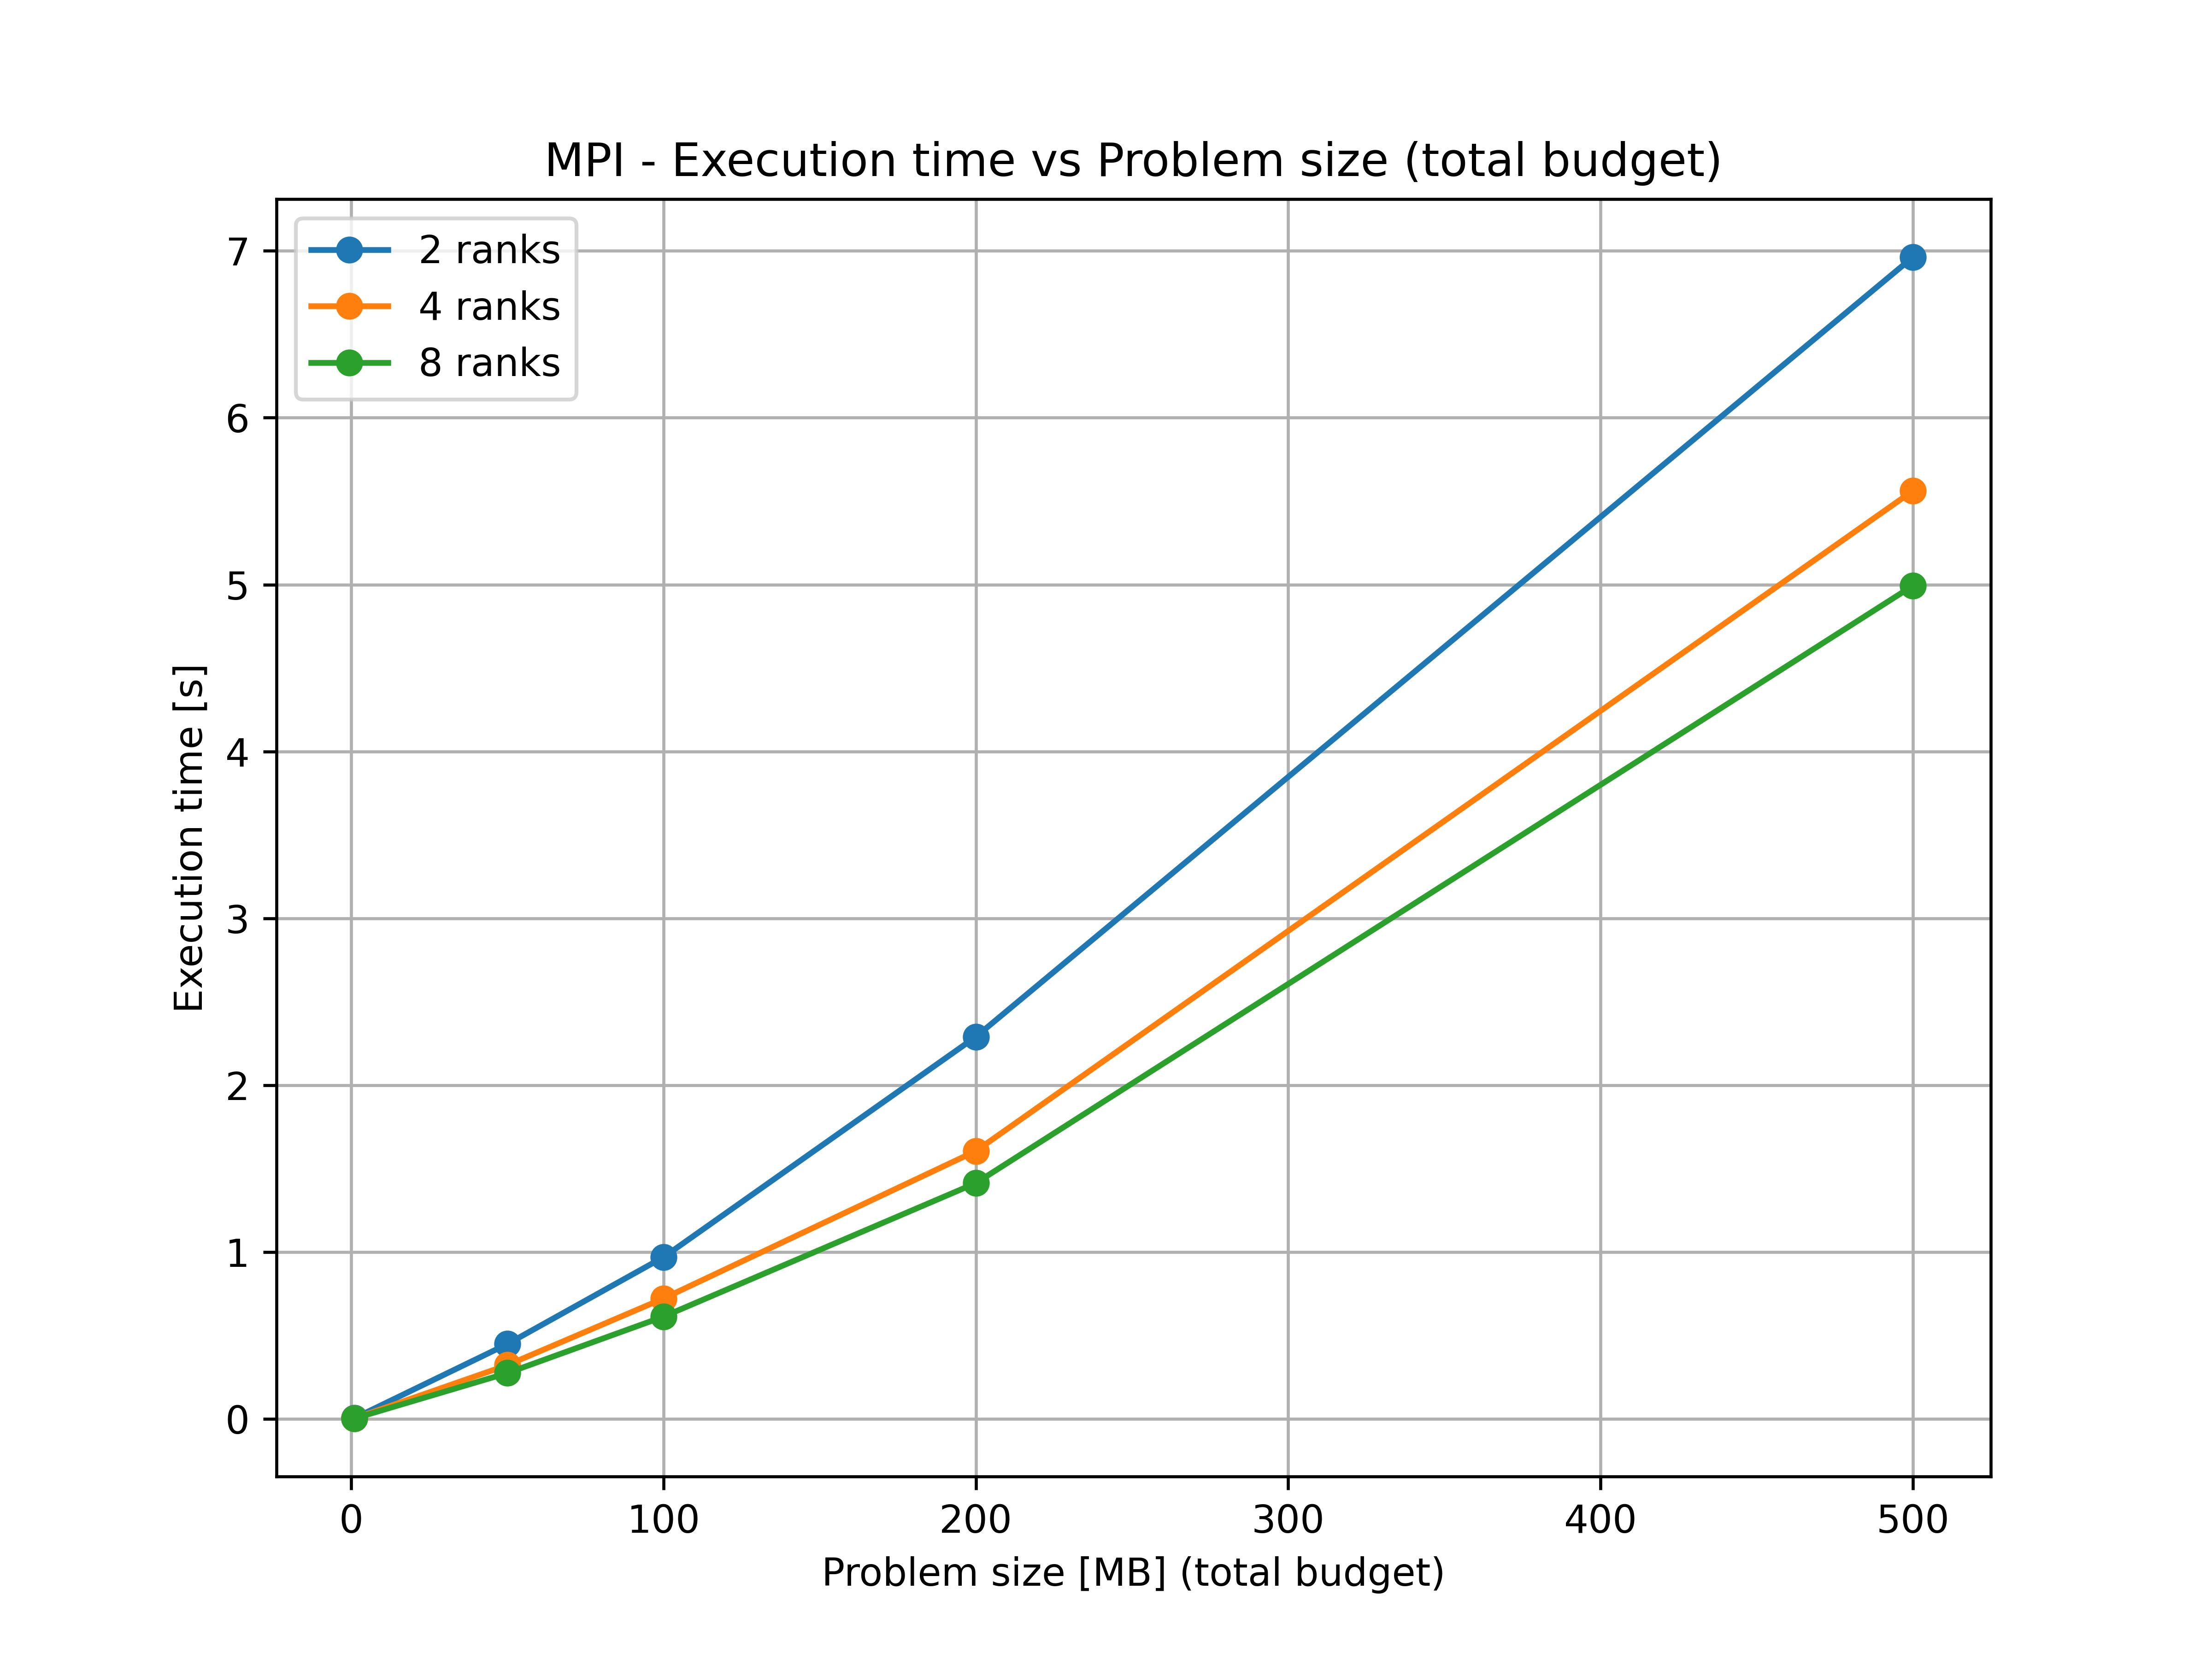
\includegraphics[width=\textwidth]{img/mpi_plots/mpi_times.jpg}
					\caption{Tempi MPI}
					\label{fig:mpi_times}
				\end{minipage}
				\hfill
				\begin{minipage}[t]{0.49\textwidth}
					\centering
					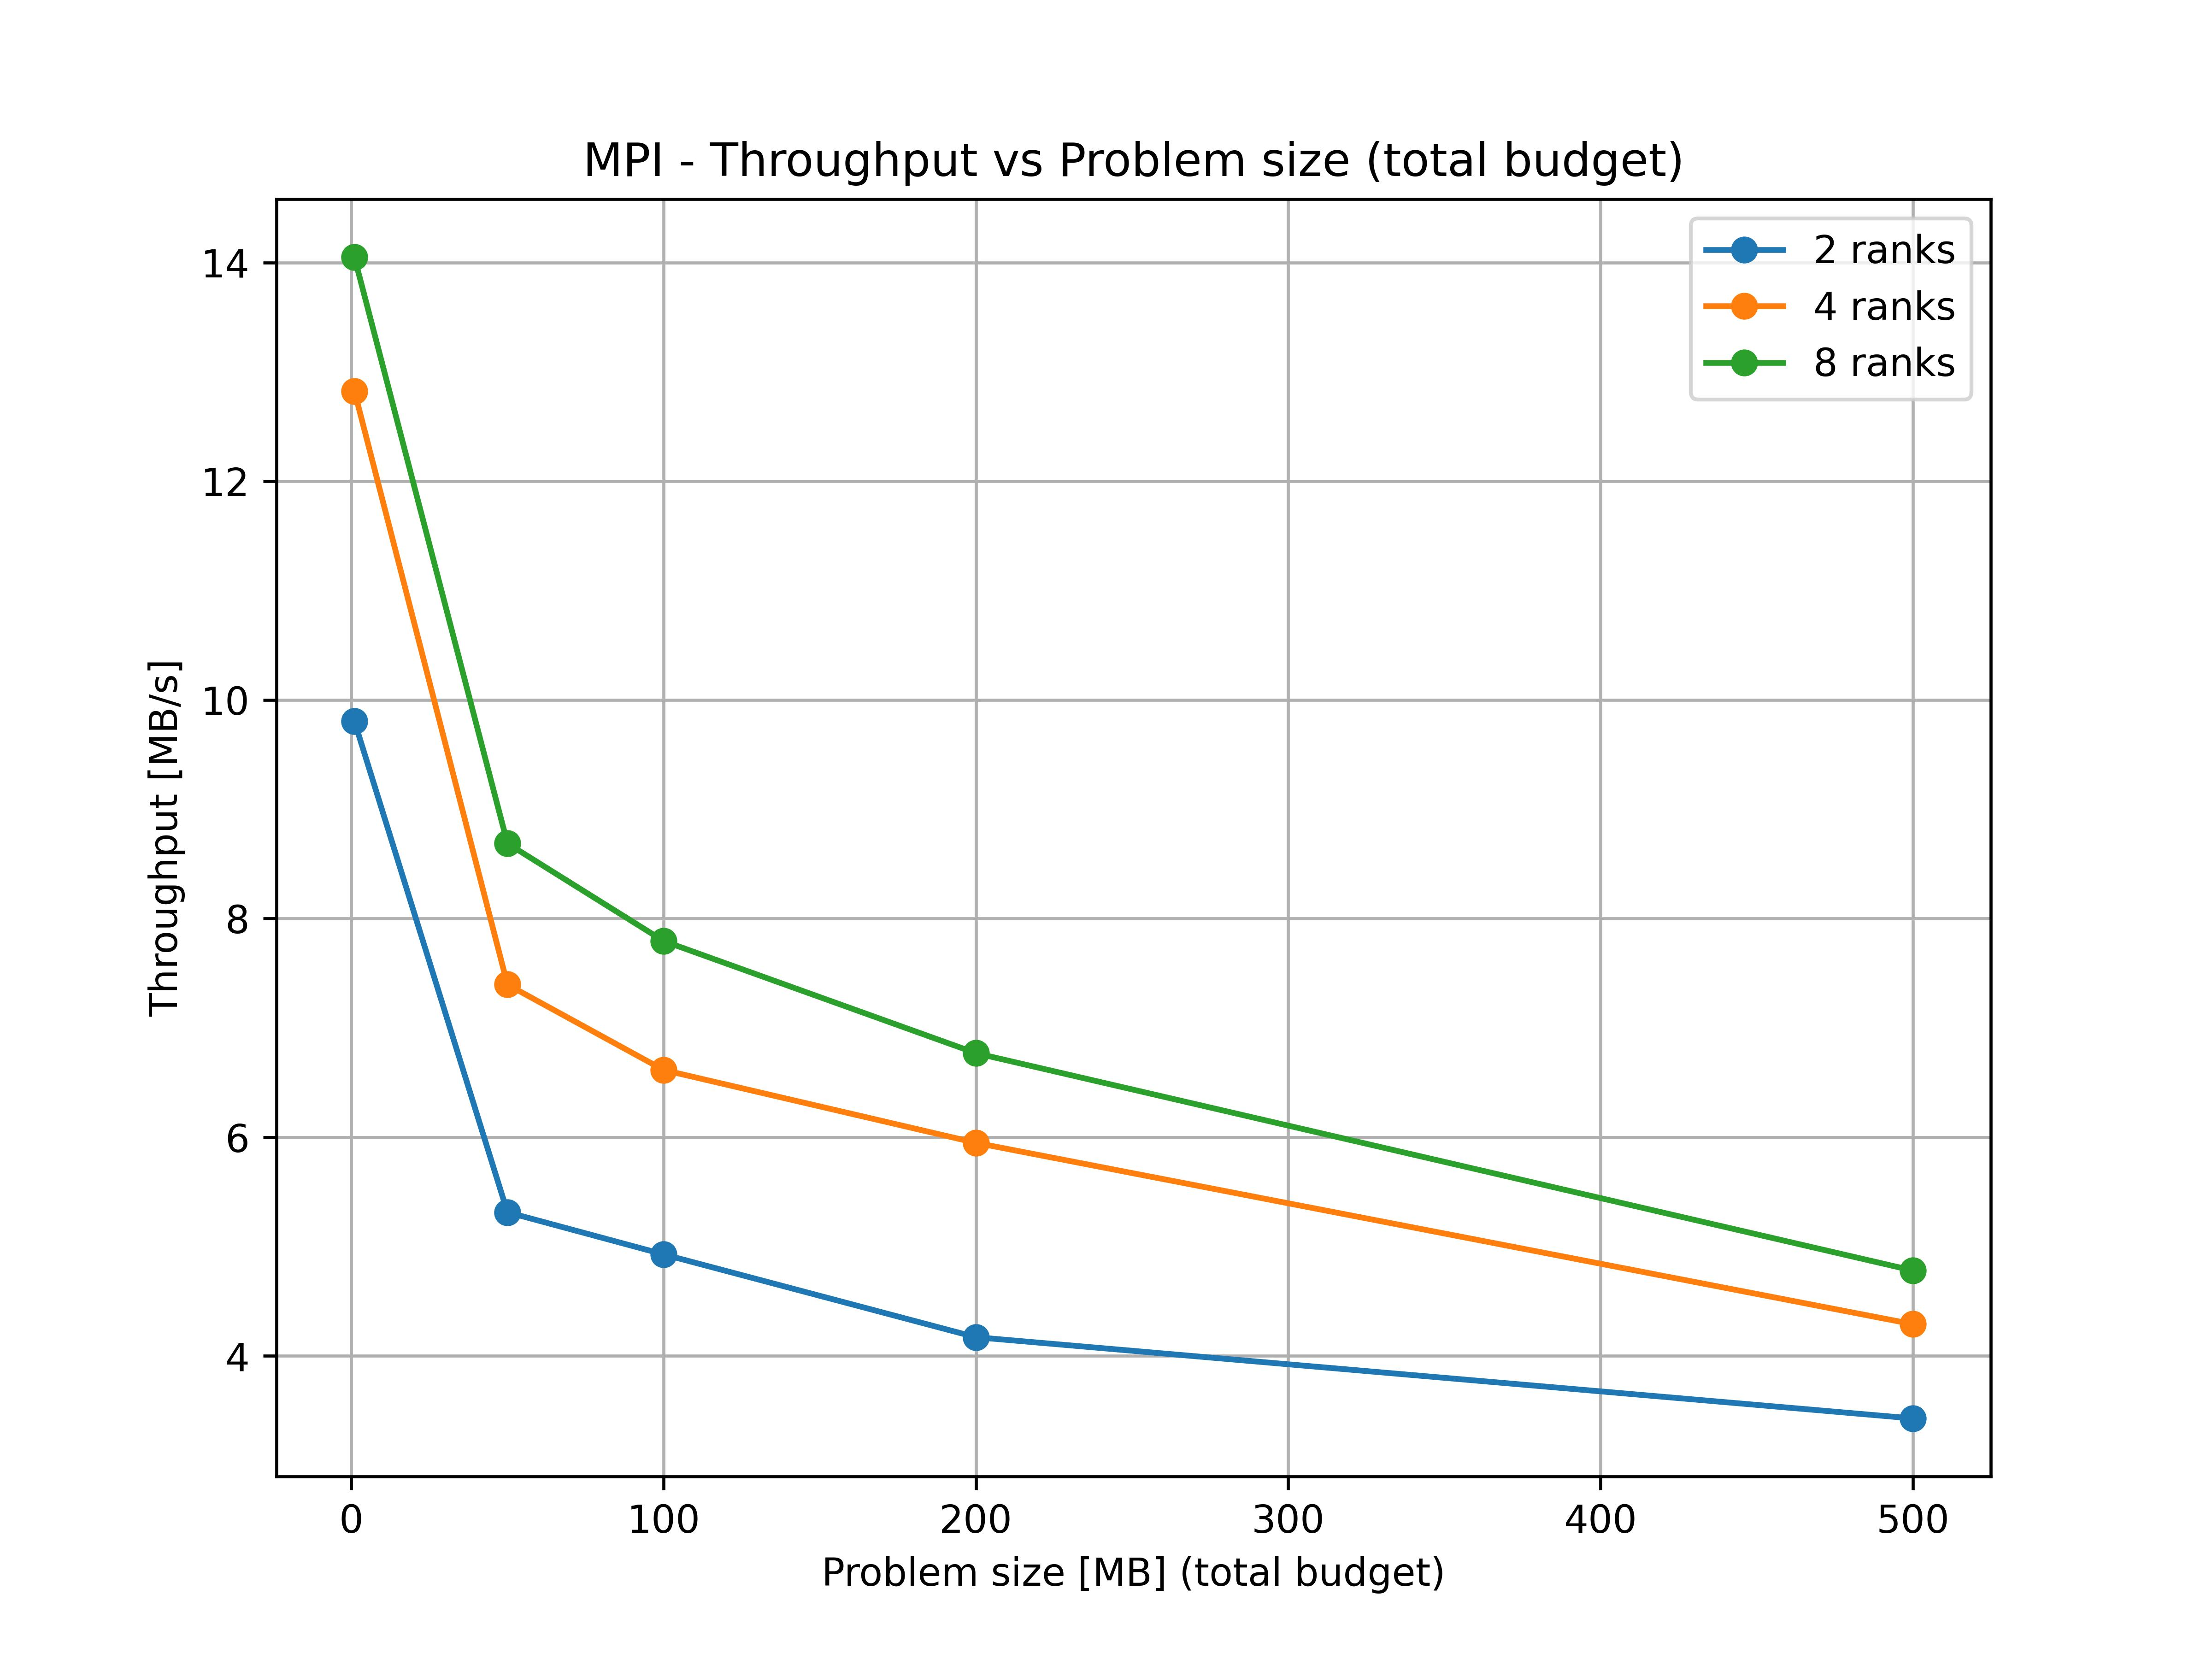
\includegraphics[width=\textwidth]{img/mpi_plots/mpi_throughput.jpg}
					\caption{Throughput MPI}
					\label{fig:mpi_throughput}
				\end{minipage}
			\end{figure}
			
			\begin{figure}[H]
				\centering
				\begin{minipage}[t]{0.49\textwidth}
					\centering
					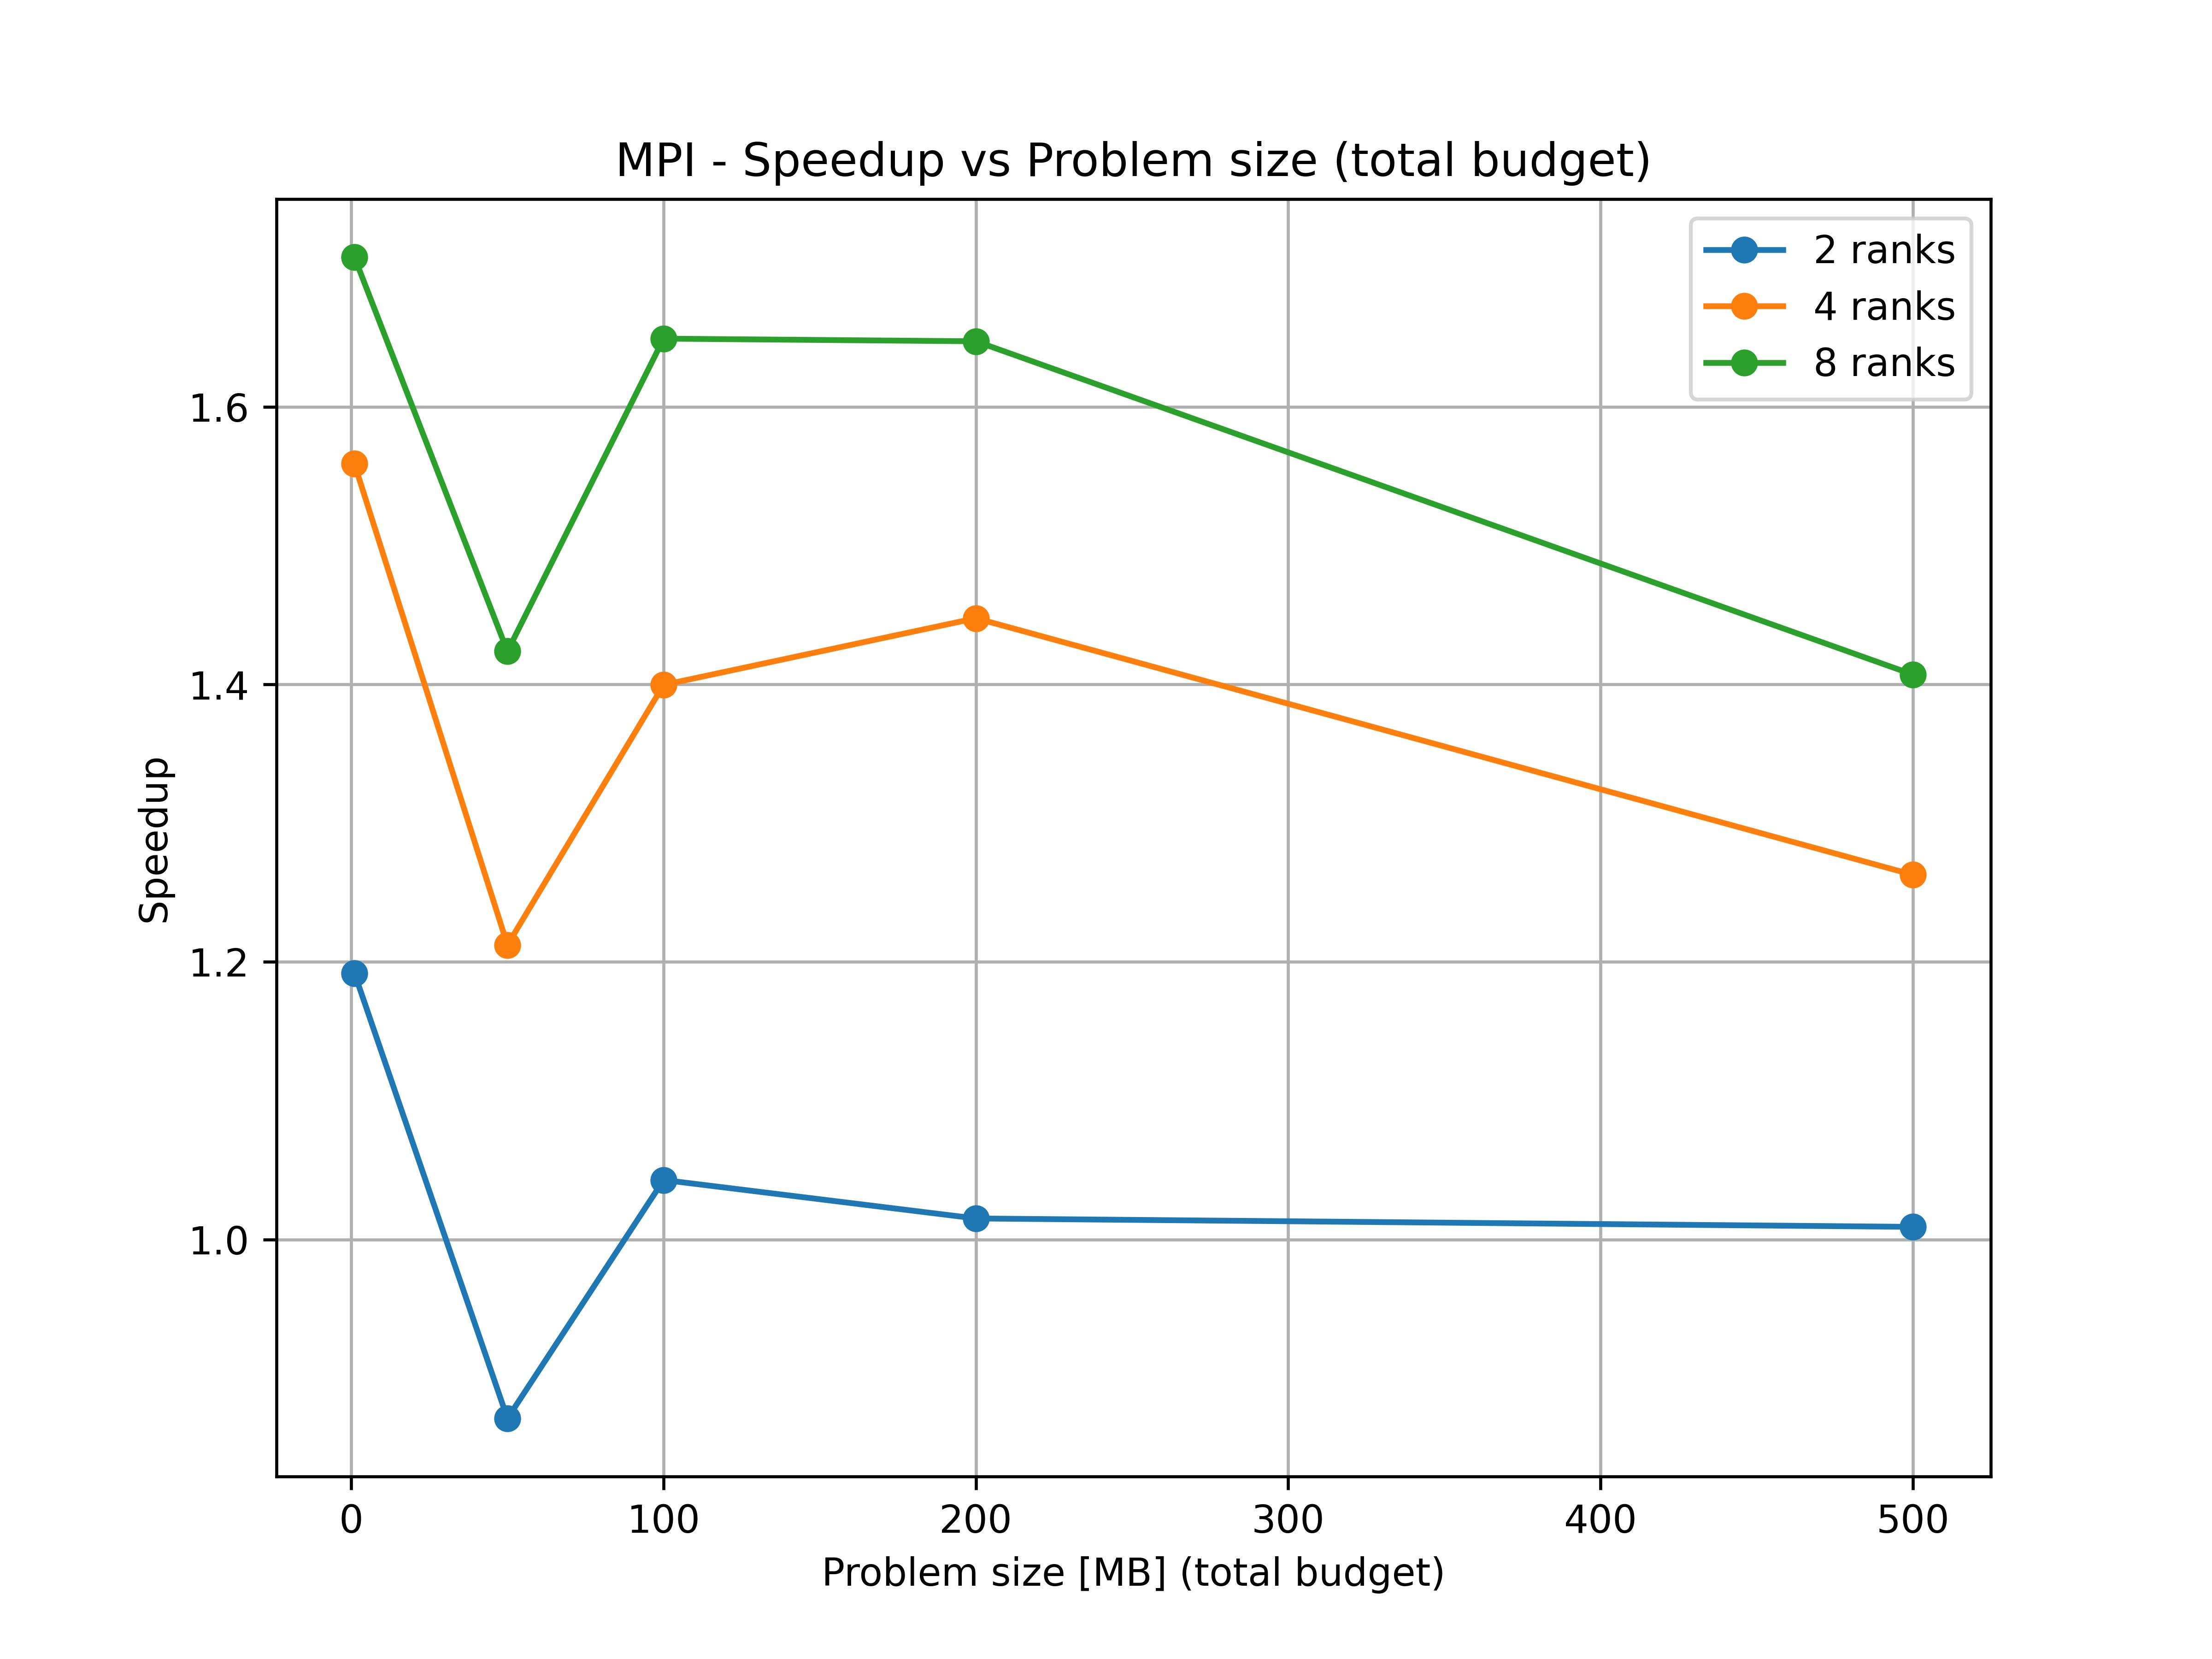
\includegraphics[width=\textwidth]{img/mpi_plots/mpi_speedup.jpg}
					\caption{Speedup MPI}
					\label{fig:mpi_speedup}
				\end{minipage}
				\hfill
				\begin{minipage}[t]{0.49\textwidth}
					\centering
					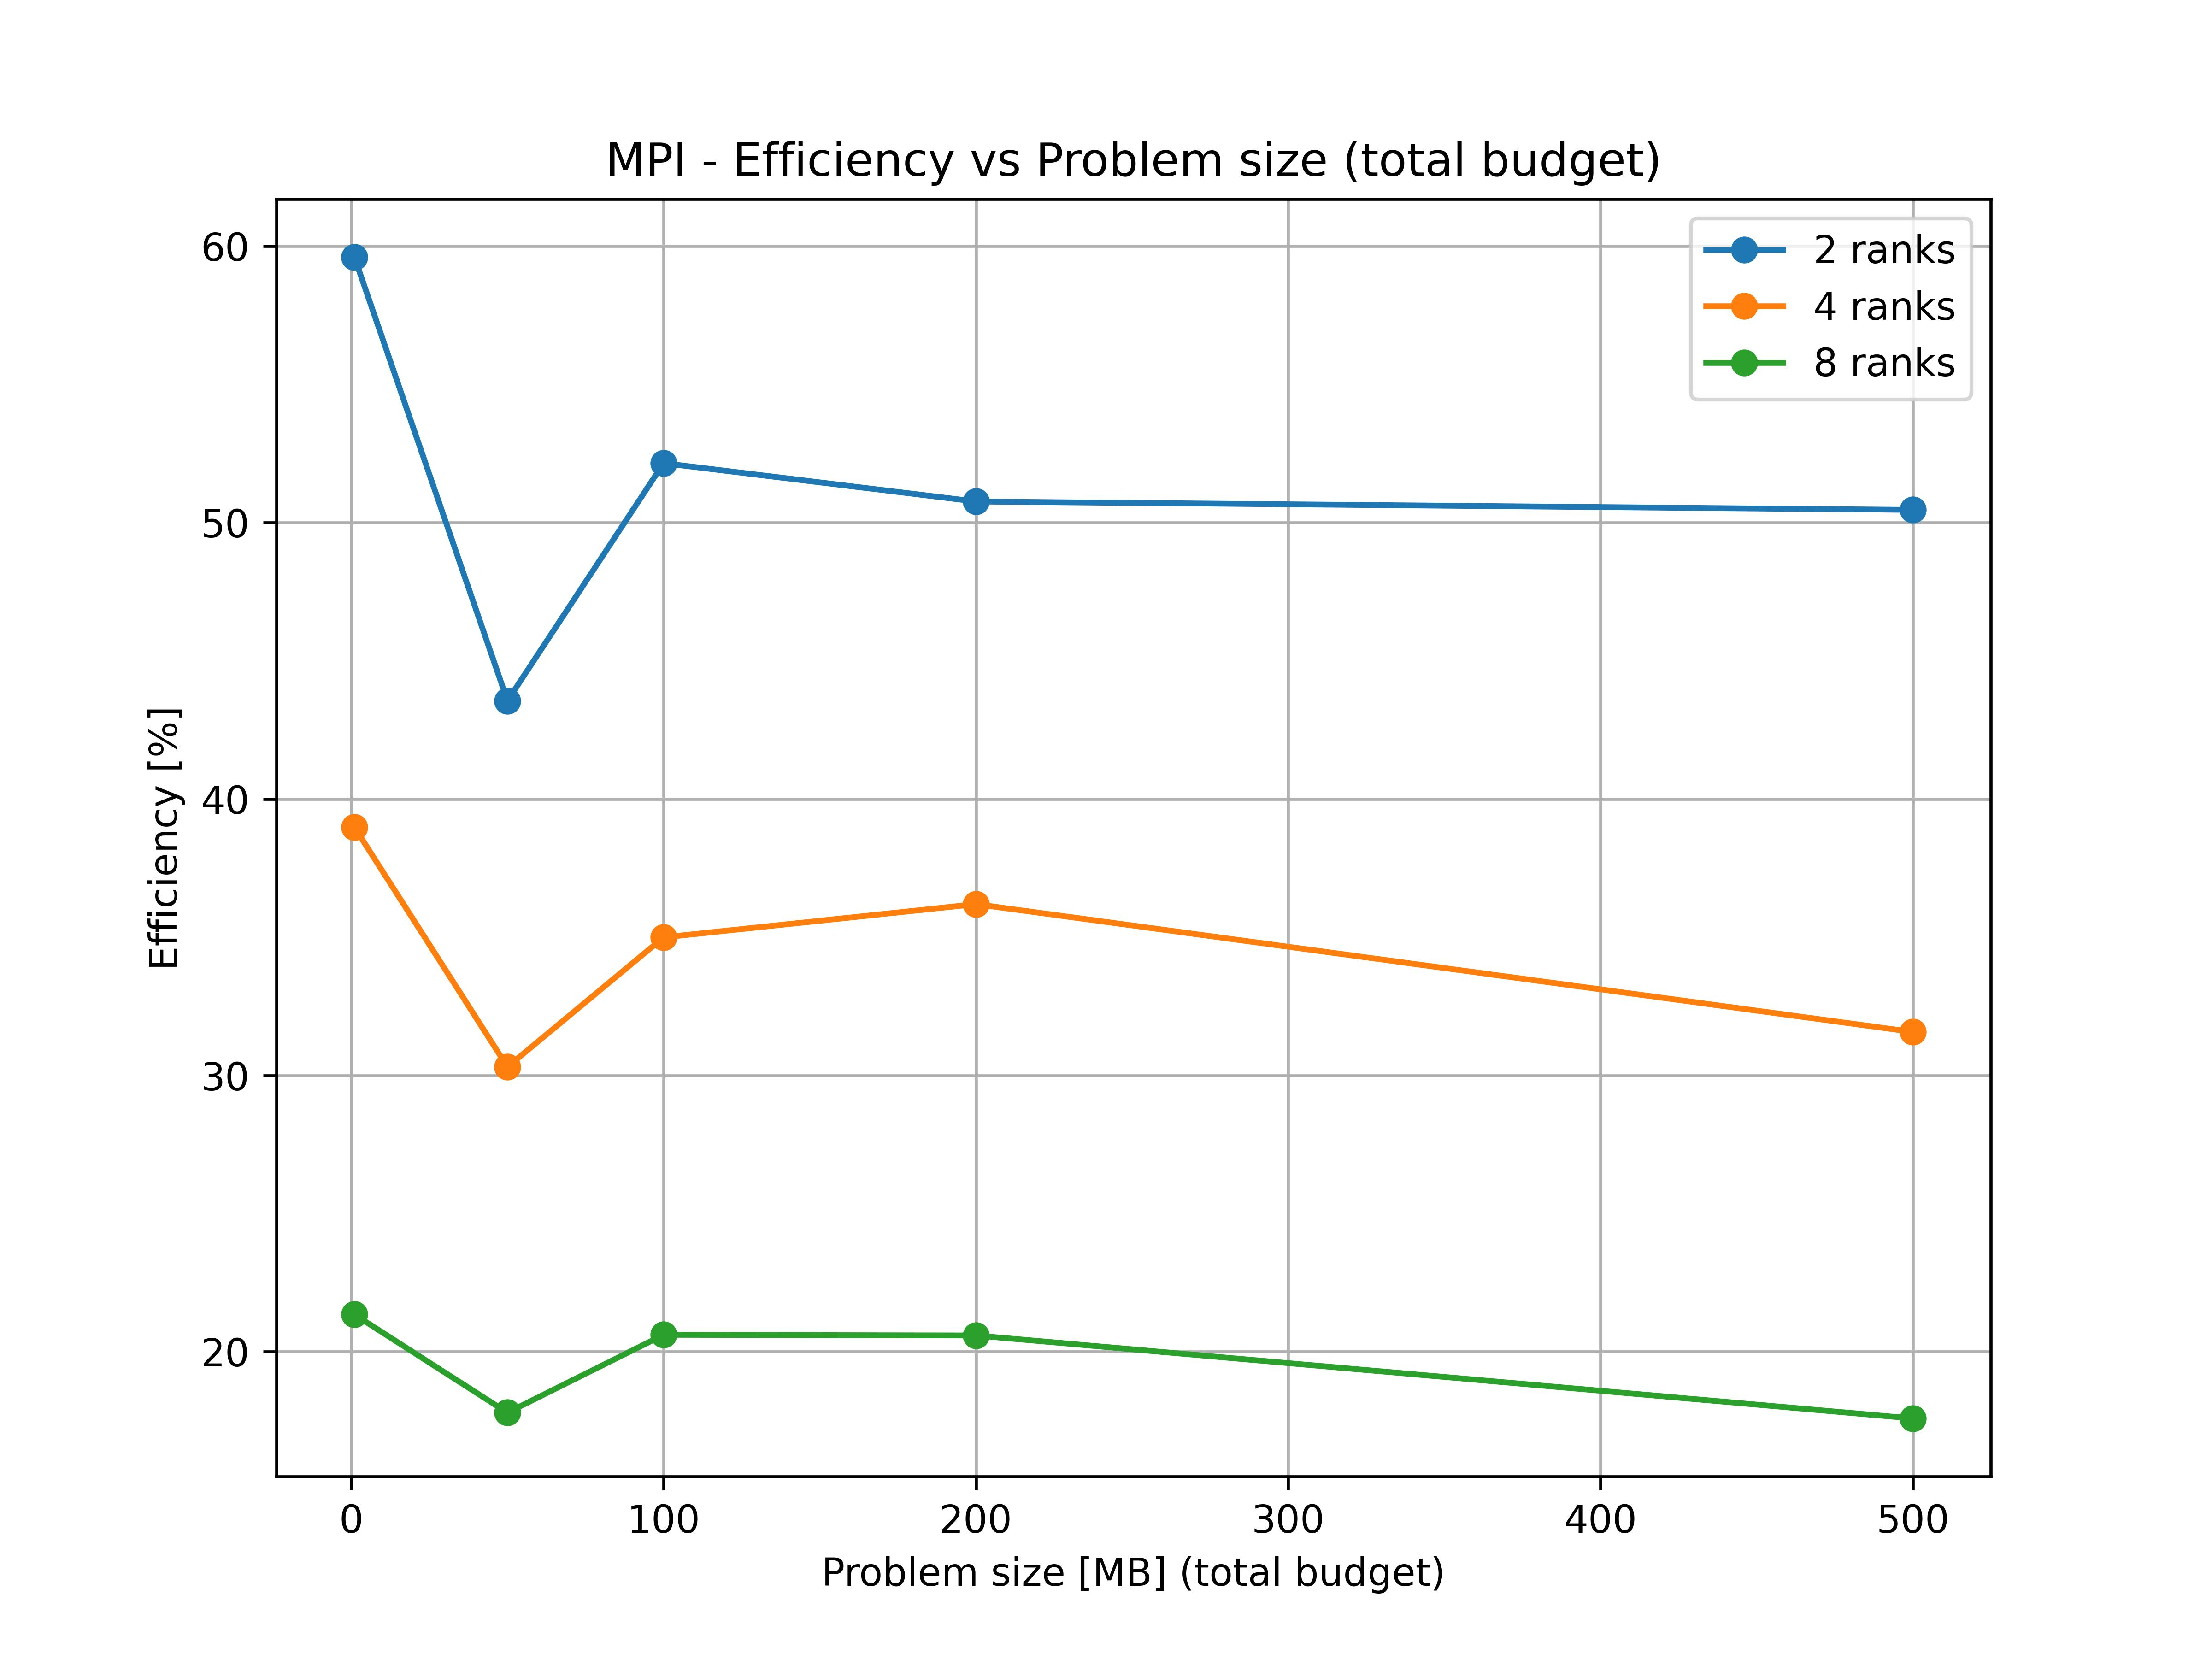
\includegraphics[width=\textwidth]{img/mpi_plots/mpi_efficiency.jpg}
					\caption{Efficiency MPI}
					\label{fig:mpi_efficiency}
				\end{minipage}
			\end{figure}
			
			\subsubsection*{Osservazioni}
				\begin{itemize}
						\item Lo \textbf{speedup} cresce con i ranks, fino a \(\sim 1.65\times\) con 8 processi su 200 MB.
						\item L’\textbf{efficienza} cala: circa \(50\%\) con 2 ranks, \(30\%\) con 4 e sotto il \(20\%\) con 8.
						\item I guadagni sono più marcati su dataset grandi (es.\ 500 MB: da $7.0s$ seq a $5.0s$ con 8 ranks).
						\item Il merge e il calcolo LCP globale restano i principali colli di bottiglia.
				\end{itemize}
		
		\subsection{Profiling della memoria}
			Il profiling con \texttt{valgrind --tool=massif} è stato condotto sul dataset da 500 MB (rank~0).
			I picchi osservati sono:
			
			\begin{itemize}
				\item \textbf{2 ranks}: \(\sim 1.54\) GB, con gran parte della memoria nei vettori \texttt{sa}, \texttt{rk}, \texttt{lcp}.
				\item \textbf{4 ranks}: \(\sim 592\) MB, footprint distribuito più equilibrato.
				\item \textbf{8 ranks}: \(\sim 577\) MB, ma con fasi di merge che portano temporanei picchi fino a \(\sim 405\) MB aggiuntivi.
			\end{itemize}
			
			\begin{figure}[H]
				\centering
				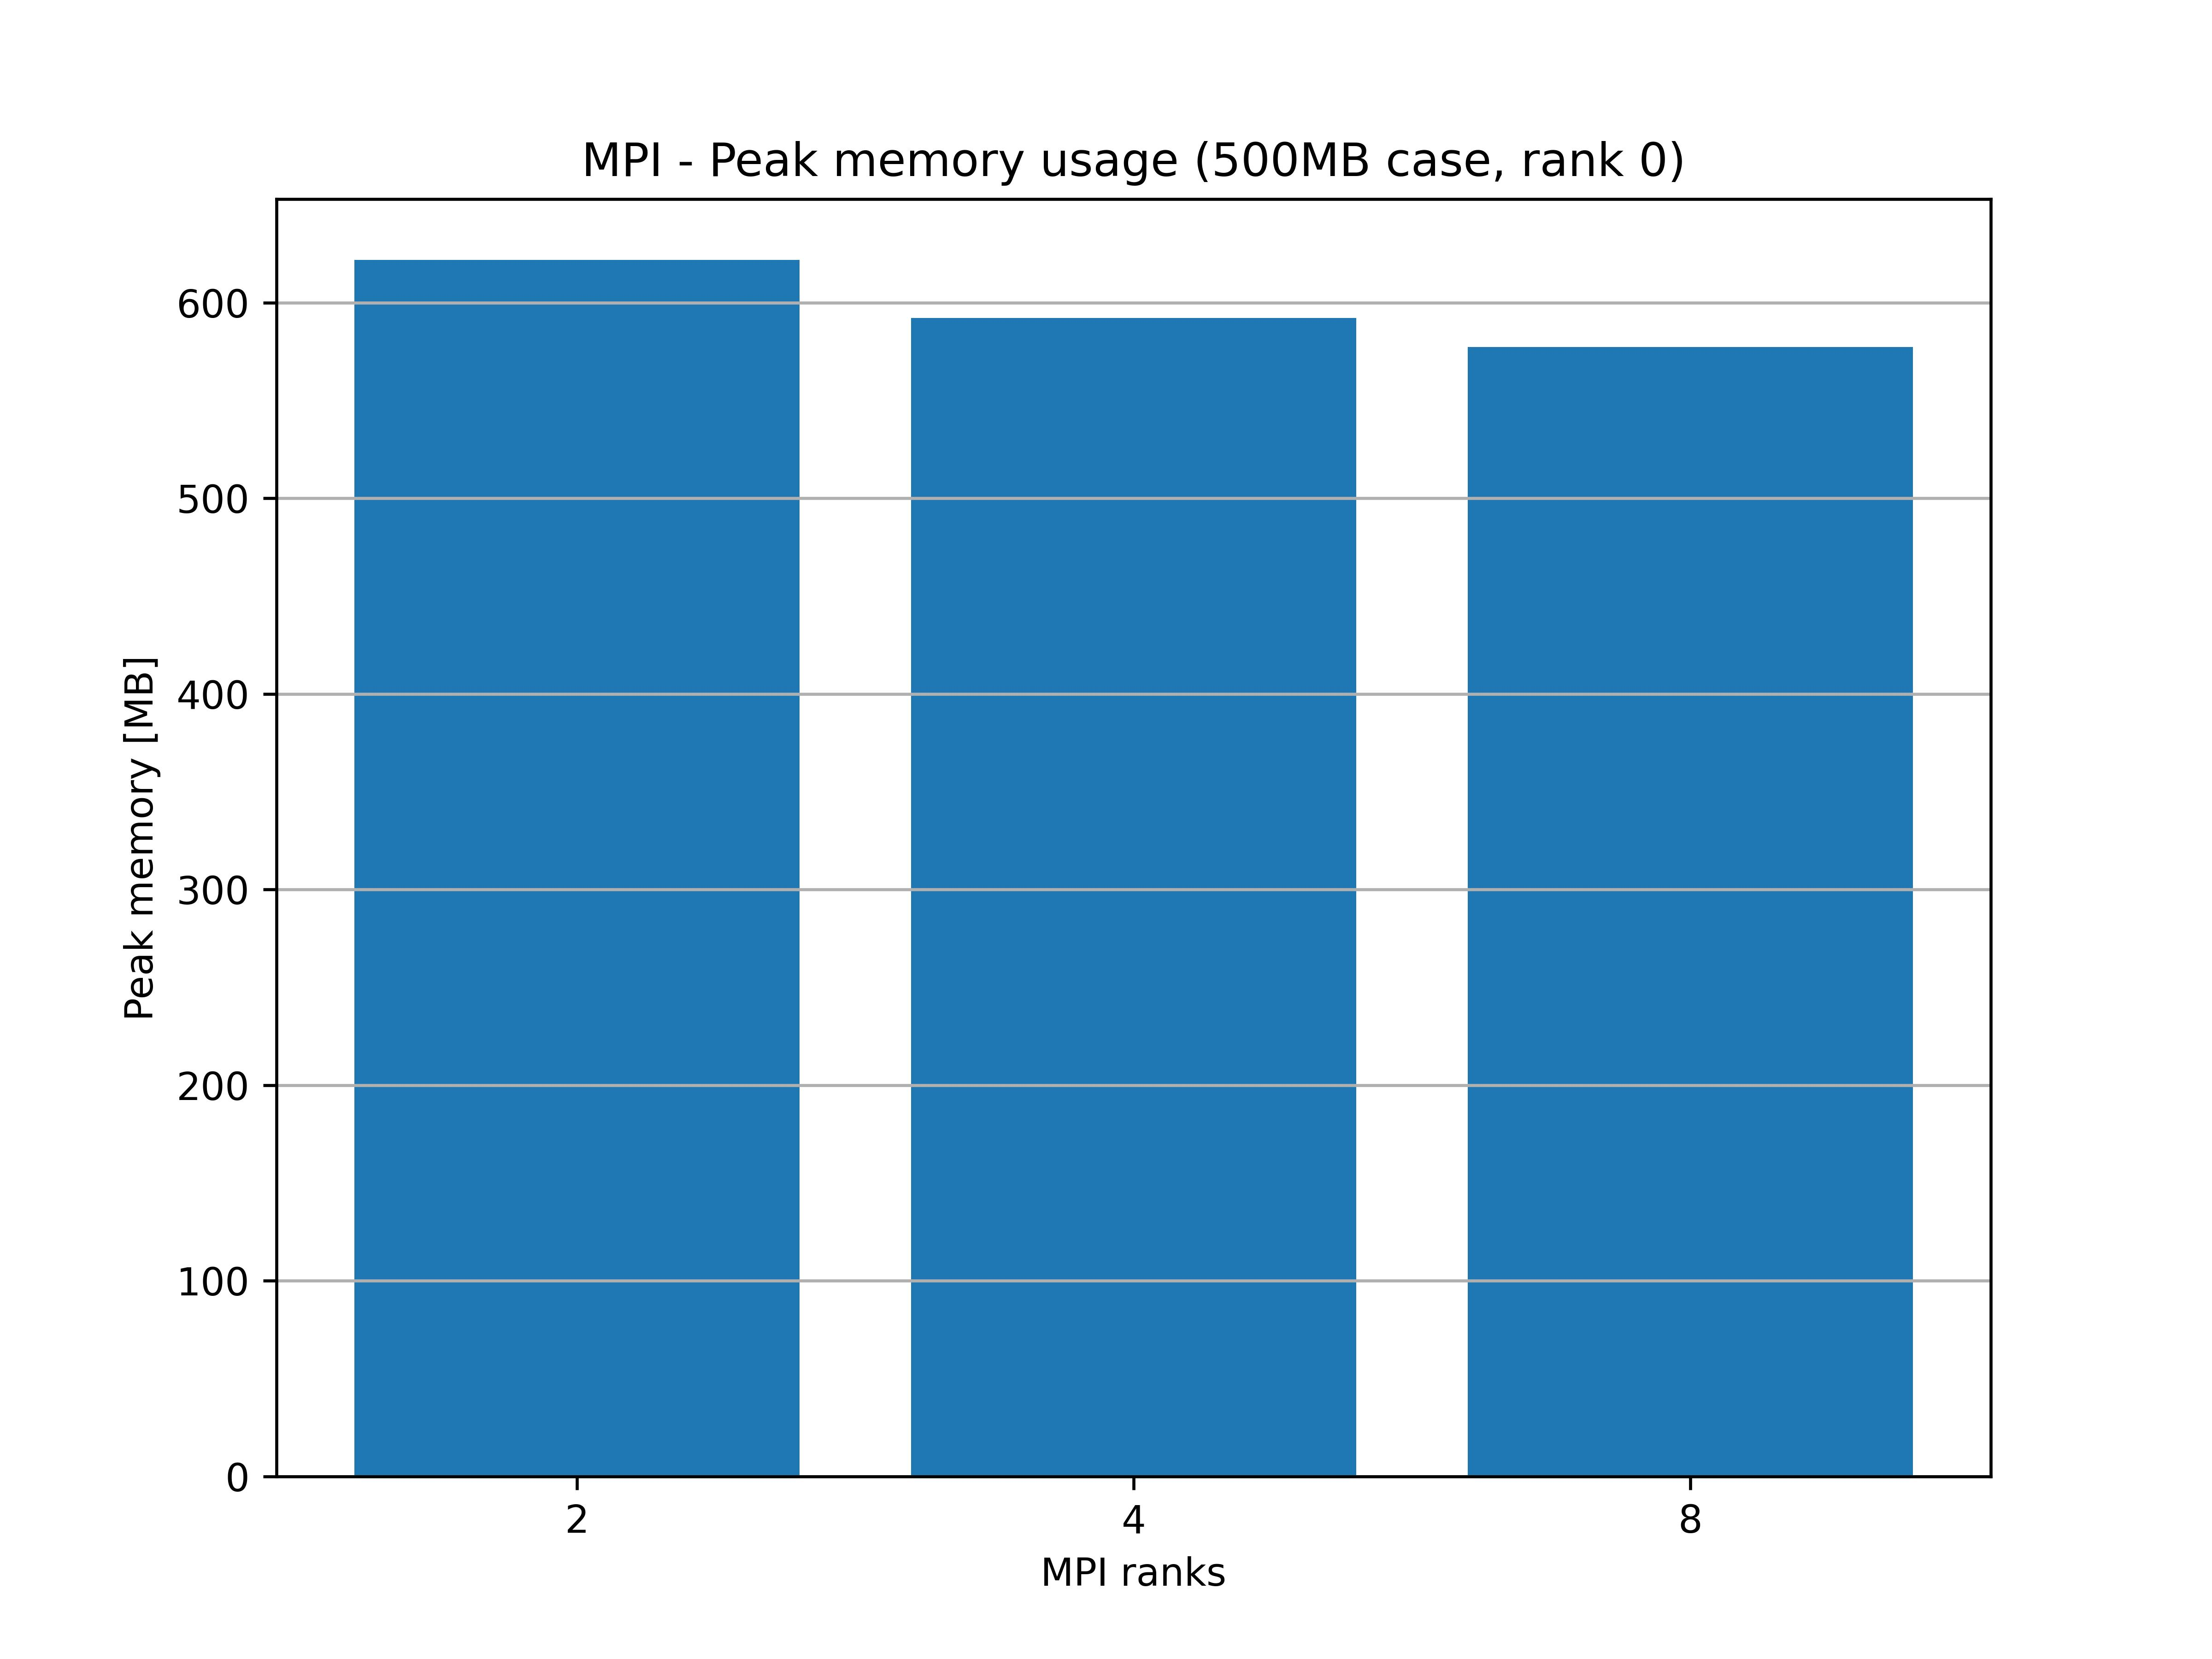
\includegraphics[width=1\linewidth]{img/mpi_plots/mpi_memory.jpg}
				\caption{Memory usage MPI (profiling Massif su rank~0)}
				\label{fig:mpi_mem_usage}
			\end{figure}
			
			\subsubsection*{Conclusione}
				La versione MPI riduce i tempi per input grandi, ma lo scaling è sub-lineare: l’efficienza si abbassa rapidamente oltre i 4 ranks.
				La memoria locale per processo diminuisce all’aumentare dei ranks, ma il rank~0 continua a mostrare picchi elevati durante il merge,
				confermando i limiti intrinseci dell’approccio distribuito.
	
	\section{Versione MPI+OpenMP}
		
		\subsection{Analisi dei tempi}
			Le prestazioni della versione ibrida sono state raccolte con cinque configurazioni ranks $\times$ threads:
			\begin{itemize}
				\item 2 ranks $\times$ 4 threads,
				\item 2 ranks $\times$ 8 threads,
				\item 4 ranks $\times$ 2 threads,
				\item 4 ranks $\times$ 4 threads,
				\item 8 ranks $\times$ 2 threads.
			\end{itemize}
			I risultati medi (10 run) sono riportati nella Tabella~\ref{tab:mpi-omp-summary}.
			
			\begin{table}[H]
				\centering
				\resizebox{\textwidth}{!}{%
					\begin{tabular}{lrrrrr rrrrr rrrrr rrrrr rrrrr}
						\toprule
						& \multicolumn{5}{c}{\textbf{2r$\times$4t}} & \multicolumn{5}{c}{\textbf{2r$\times$8t}} & \multicolumn{5}{c}{\textbf{4r$\times$2t}} & \multicolumn{5}{c}{\textbf{4r$\times$4t}} & \multicolumn{5}{c}{\textbf{8r$\times$2t}} \\
						\cmidrule(lr){2-6}\cmidrule(lr){7-11}\cmidrule(lr){12-16}\cmidrule(lr){17-21}\cmidrule(lr){22-26}
						\textbf{Size} & \textbf{merge} & \textbf{lcp} & \textbf{comm} & \textbf{compute} & \textbf{MB/s} &
						\textbf{merge} & \textbf{lcp} & \textbf{comm} & \textbf{compute} & \textbf{MB/s} &
						\textbf{merge} & \textbf{lcp} & \textbf{comm} & \textbf{compute} & \textbf{MB/s} &
						\textbf{merge} & \textbf{lcp} & \textbf{comm} & \textbf{compute} & \textbf{MB/s} &
						\textbf{merge} & \textbf{lcp} & \textbf{comm} & \textbf{compute} & \textbf{MB/s} \\
						(MB) & (s) & (s) & (s) & (s) & &
						(s) & (s) & (s) & (s) & &
						(s) & (s) & (s) & (s) & &
						(s) & (s) & (s) & (s) & &
						(s) & (s) & (s) & (s) & \\
						\midrule
						1   & 0.00126 & 0.00051 & 0.00002 & 0.00522 & 9.13 & 0.00125 & 0.00050 & 0.00002 & 0.00550 & 8.66 & 0.00190 & 0.00058 & 0.00005 & 0.00411 & 11.59 & 0.00171 & 0.00051 & 0.00003 & 0.00401 & 11.87 & 0.00238 & 0.00060 & 0.00005 & 0.00439 & 11.31 \\
						50  & 0.08514 & 0.05296 & 0.00117 & 0.4419  & 5.39 & 0.08470 & 0.05569 & 0.00135 & 0.4440  & 5.36 & 0.11490 & 0.05455 & 0.00135 & 0.3245 & 7.34 & 0.11659 & 0.05850 & 0.00126 & 0.3330 & 7.17 & 0.14463 & 0.06297 & 0.00156 & 0.2938 & 8.15 \\
						100 & 0.18114 & 0.14643 & 0.00260 & 0.9551  & 4.99 & 0.18087 & 0.15562 & 0.00285 & 0.9755  & 4.88 & 0.24668 & 0.15889 & 0.00297 & 0.7377 & 6.46 & 0.23866 & 0.14889 & 0.00285 & 0.7201 & 6.62 & 0.28422 & 0.15587 & 0.00323 & 0.6203 & 7.70 \\
						200 & 0.44999 & 0.38690 & 0.00415 & 2.2079  & 4.32 & 0.49692 & 0.38877 & 0.00439 & 2.2665  & 4.20 & 0.55881 & 0.38123 & 0.00583 & 1.6593 & 5.75 & 0.52421 & 0.37098 & 0.00579 & 1.6103 & 5.91 & 0.69348 & 0.37936 & 0.00637 & 1.4838 & 6.43 \\
						500 & 2.24016 & 1.15297 & 0.01009 & 7.1236  & 3.34 & 2.05653 & 1.15114 & 0.01035 & 6.8713  & 3.47 & 2.61852 & 1.14213 & 0.01249 & 5.7554 & 4.14 & 2.48589 & 1.11313 & 0.01247 & 5.6125 & 4.25 & 2.83967 & 1.14664 & 0.01525 & 5.1647 & 4.61 \\
						\bottomrule
					\end{tabular}}
				\caption{MPI+OpenMP — Medie (10 run) per size e configurazione.}
				\label{tab:mpi-omp-summary}
			\end{table}
			
			\begin{figure}[H]
				\centering
				\begin{minipage}[t]{0.49\textwidth}
					\centering
					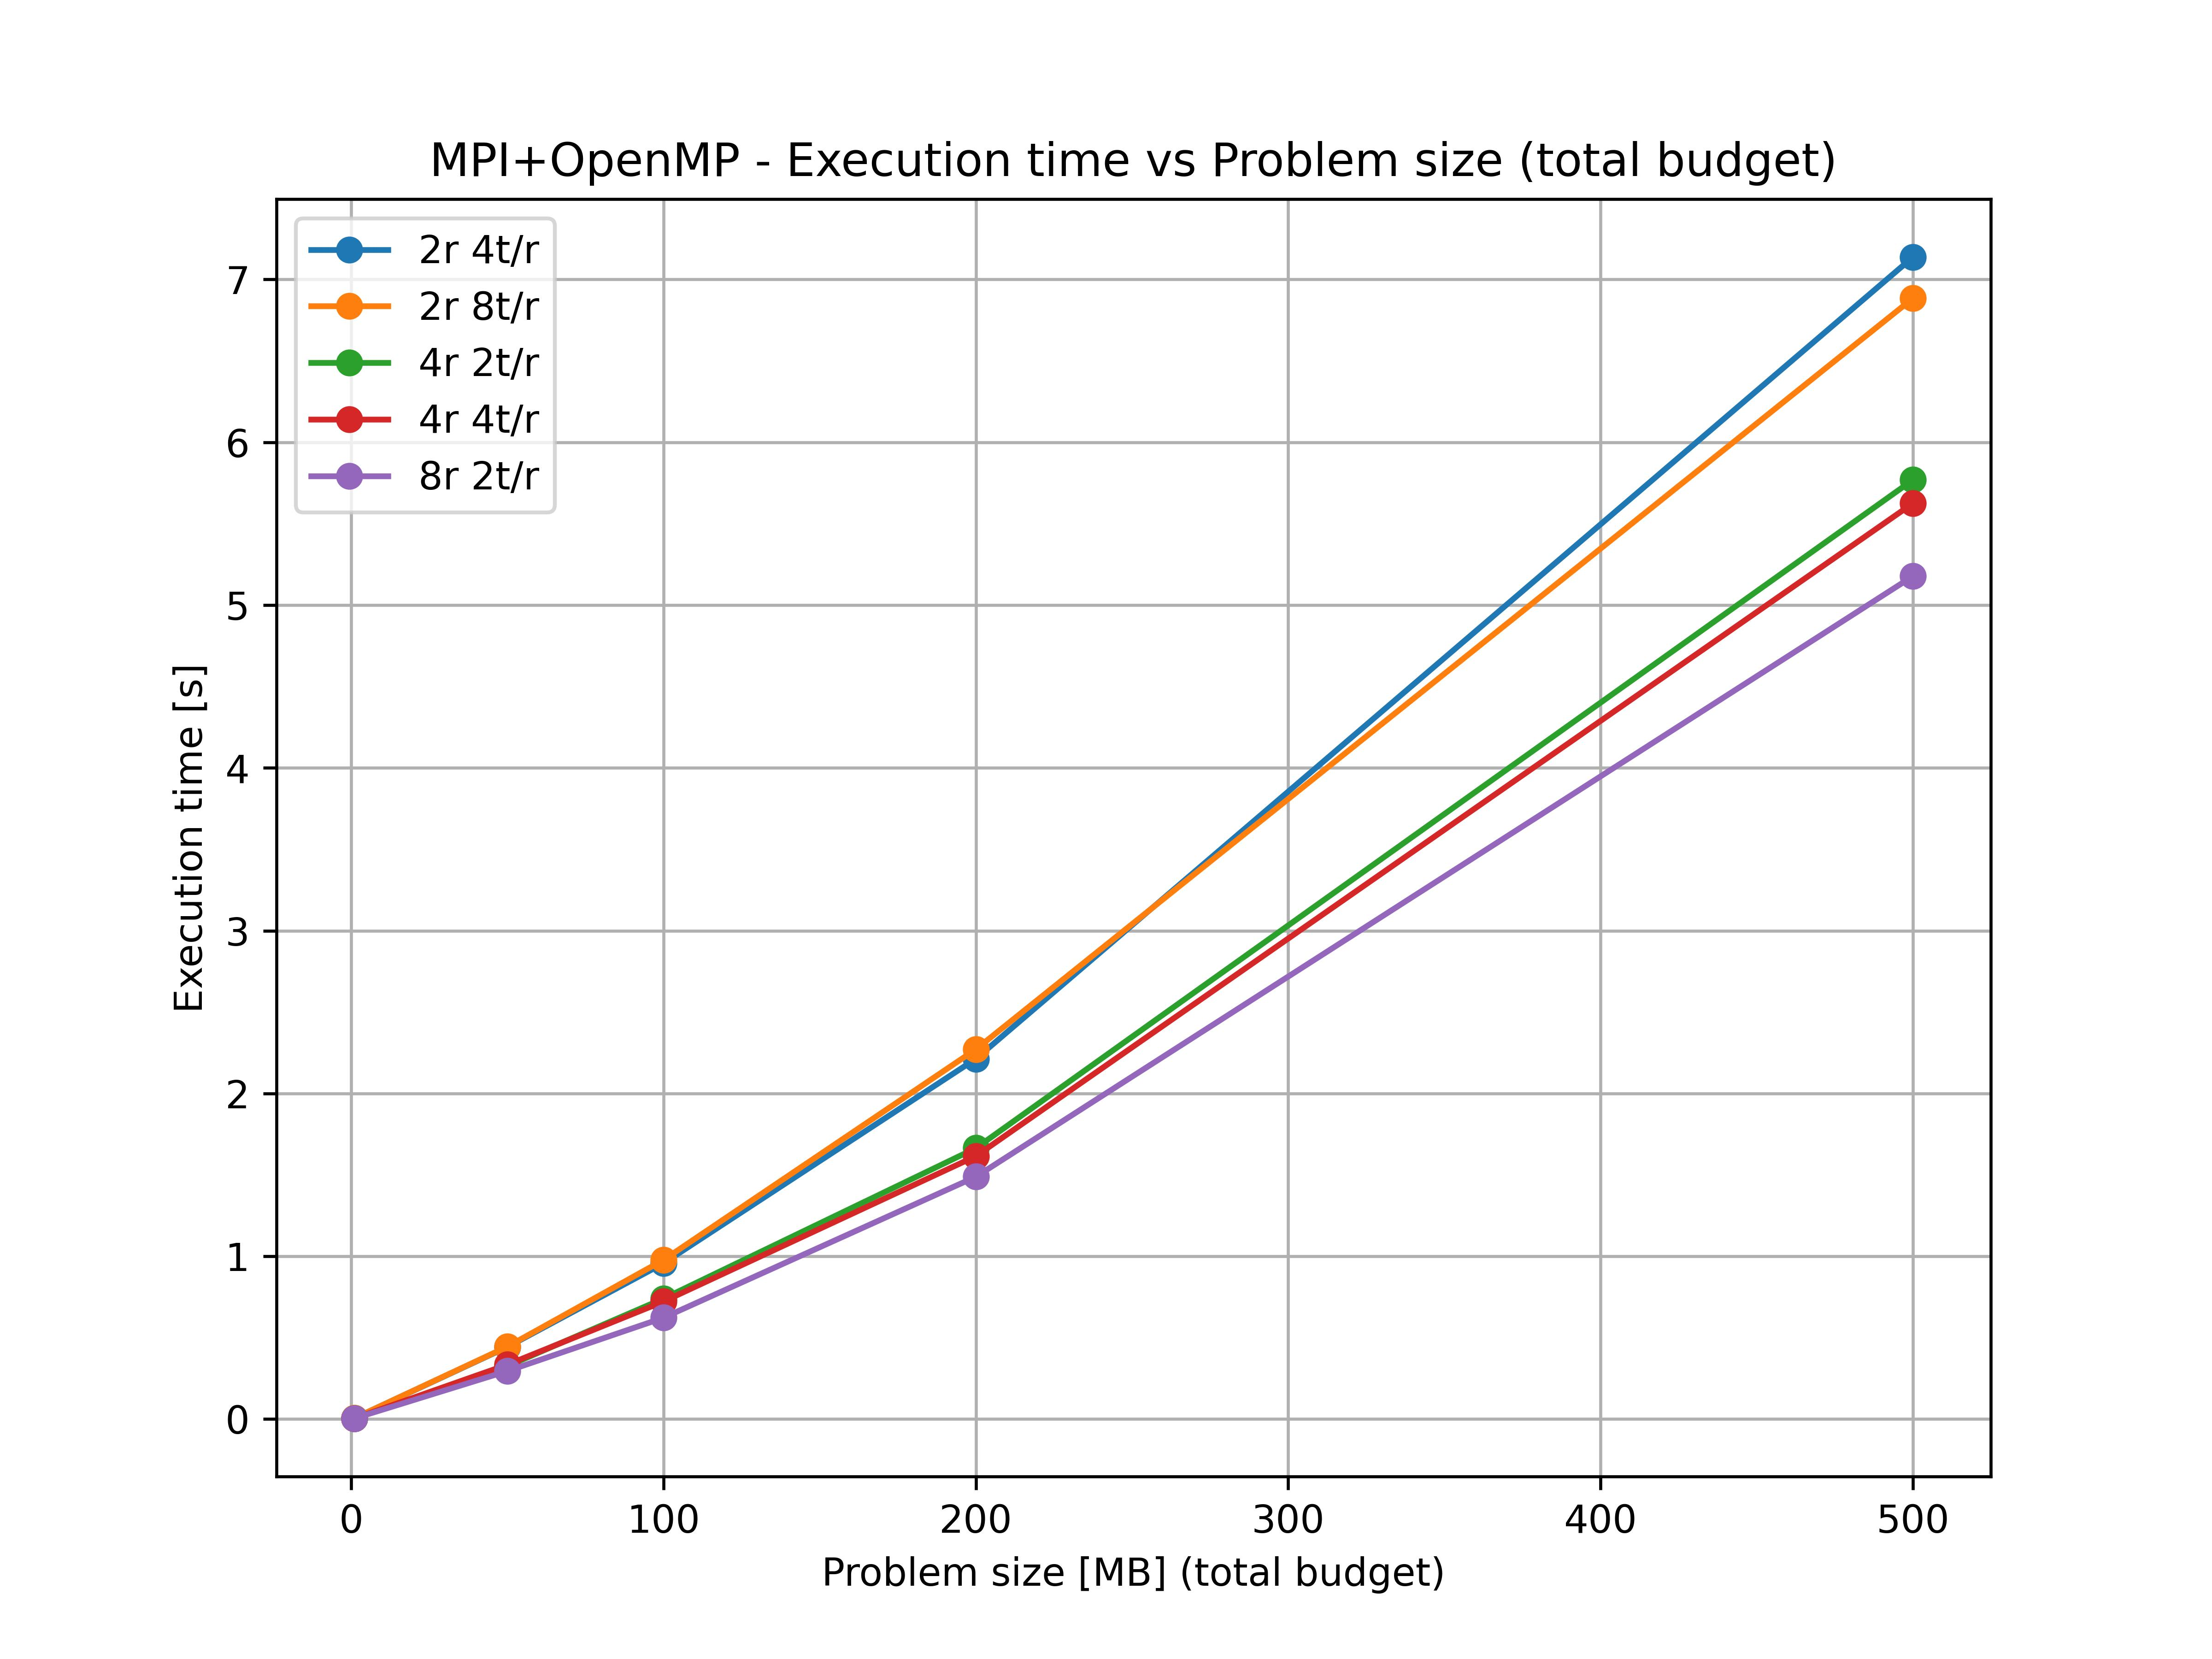
\includegraphics[width=\textwidth]{img/mpi_omp_plots/mpi_omp_times.jpg}
					\caption{Tempi MPI+OMP}
					\label{fig:mpi_omp_times}
				\end{minipage}
				\hfill
				\begin{minipage}[t]{0.49\textwidth}
					\centering
					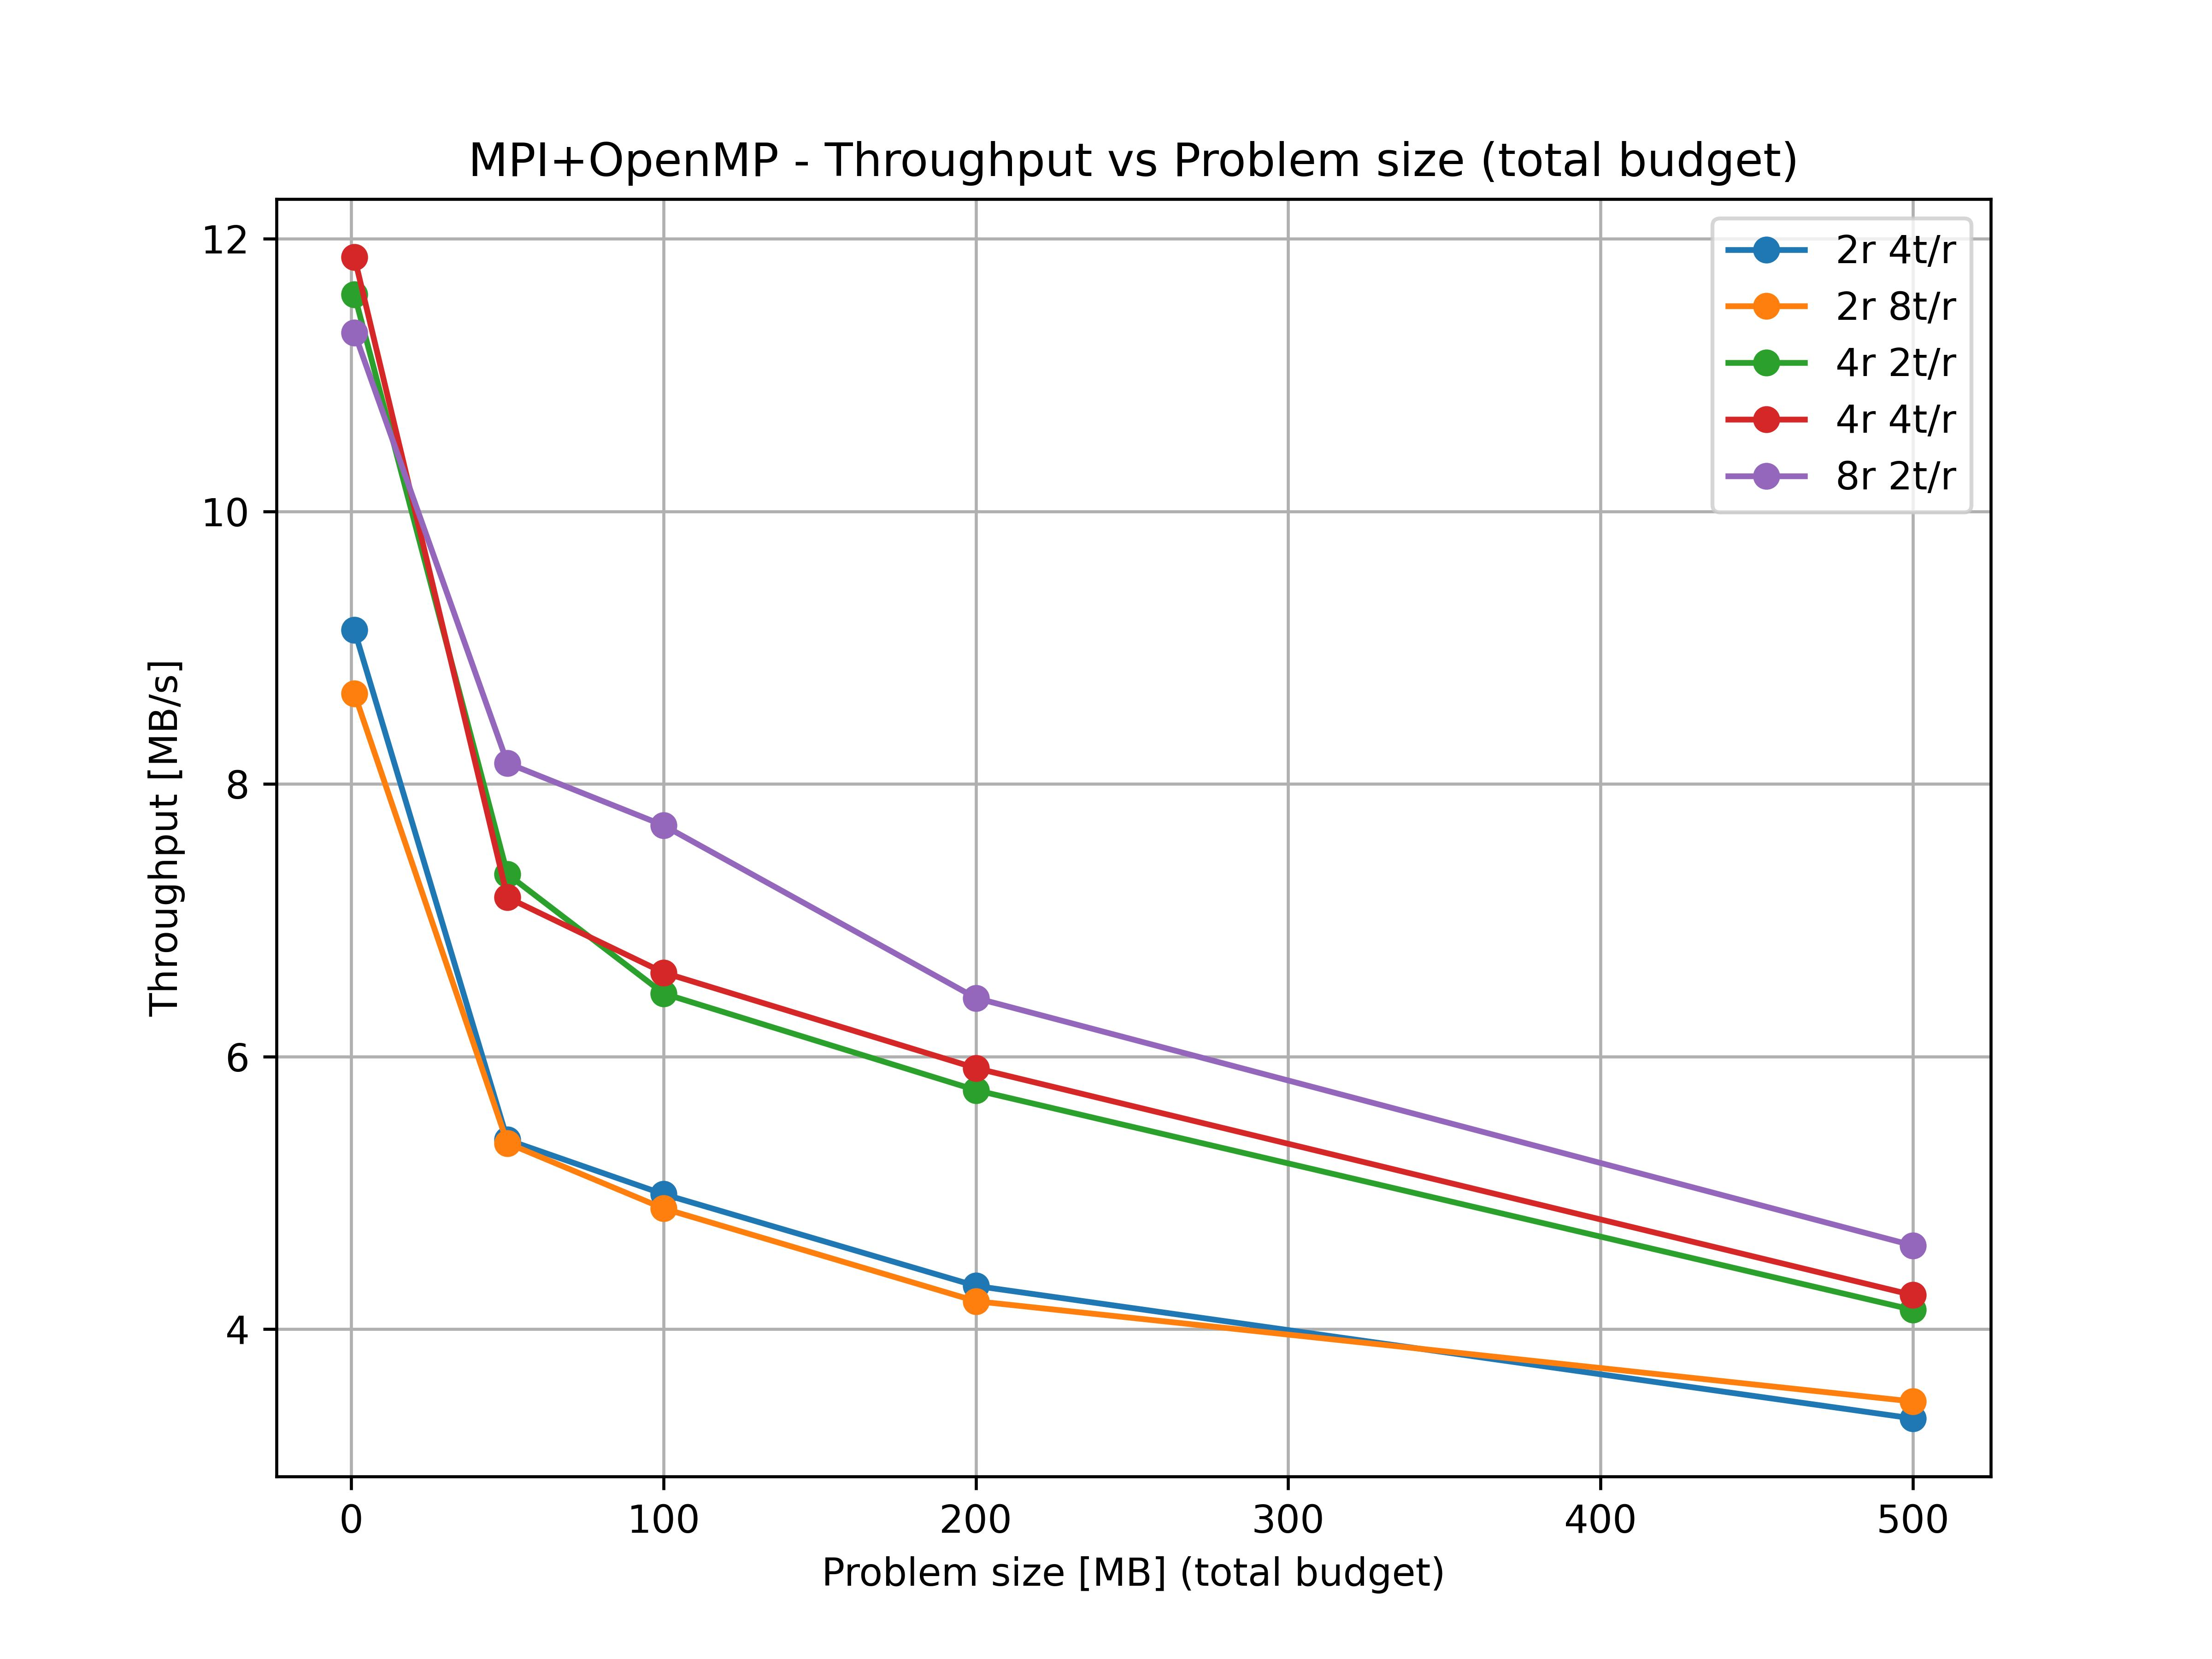
\includegraphics[width=\textwidth]{img/mpi_omp_plots/mpi_omp_throughput.jpg}
					\caption{Throughput MPI+OMP}
					\label{fig:mpi_omp_throughput}
				\end{minipage}
			\end{figure}
			
			\begin{figure}[H]
				\centering
				\begin{minipage}[t]{0.49\textwidth}
					\centering
					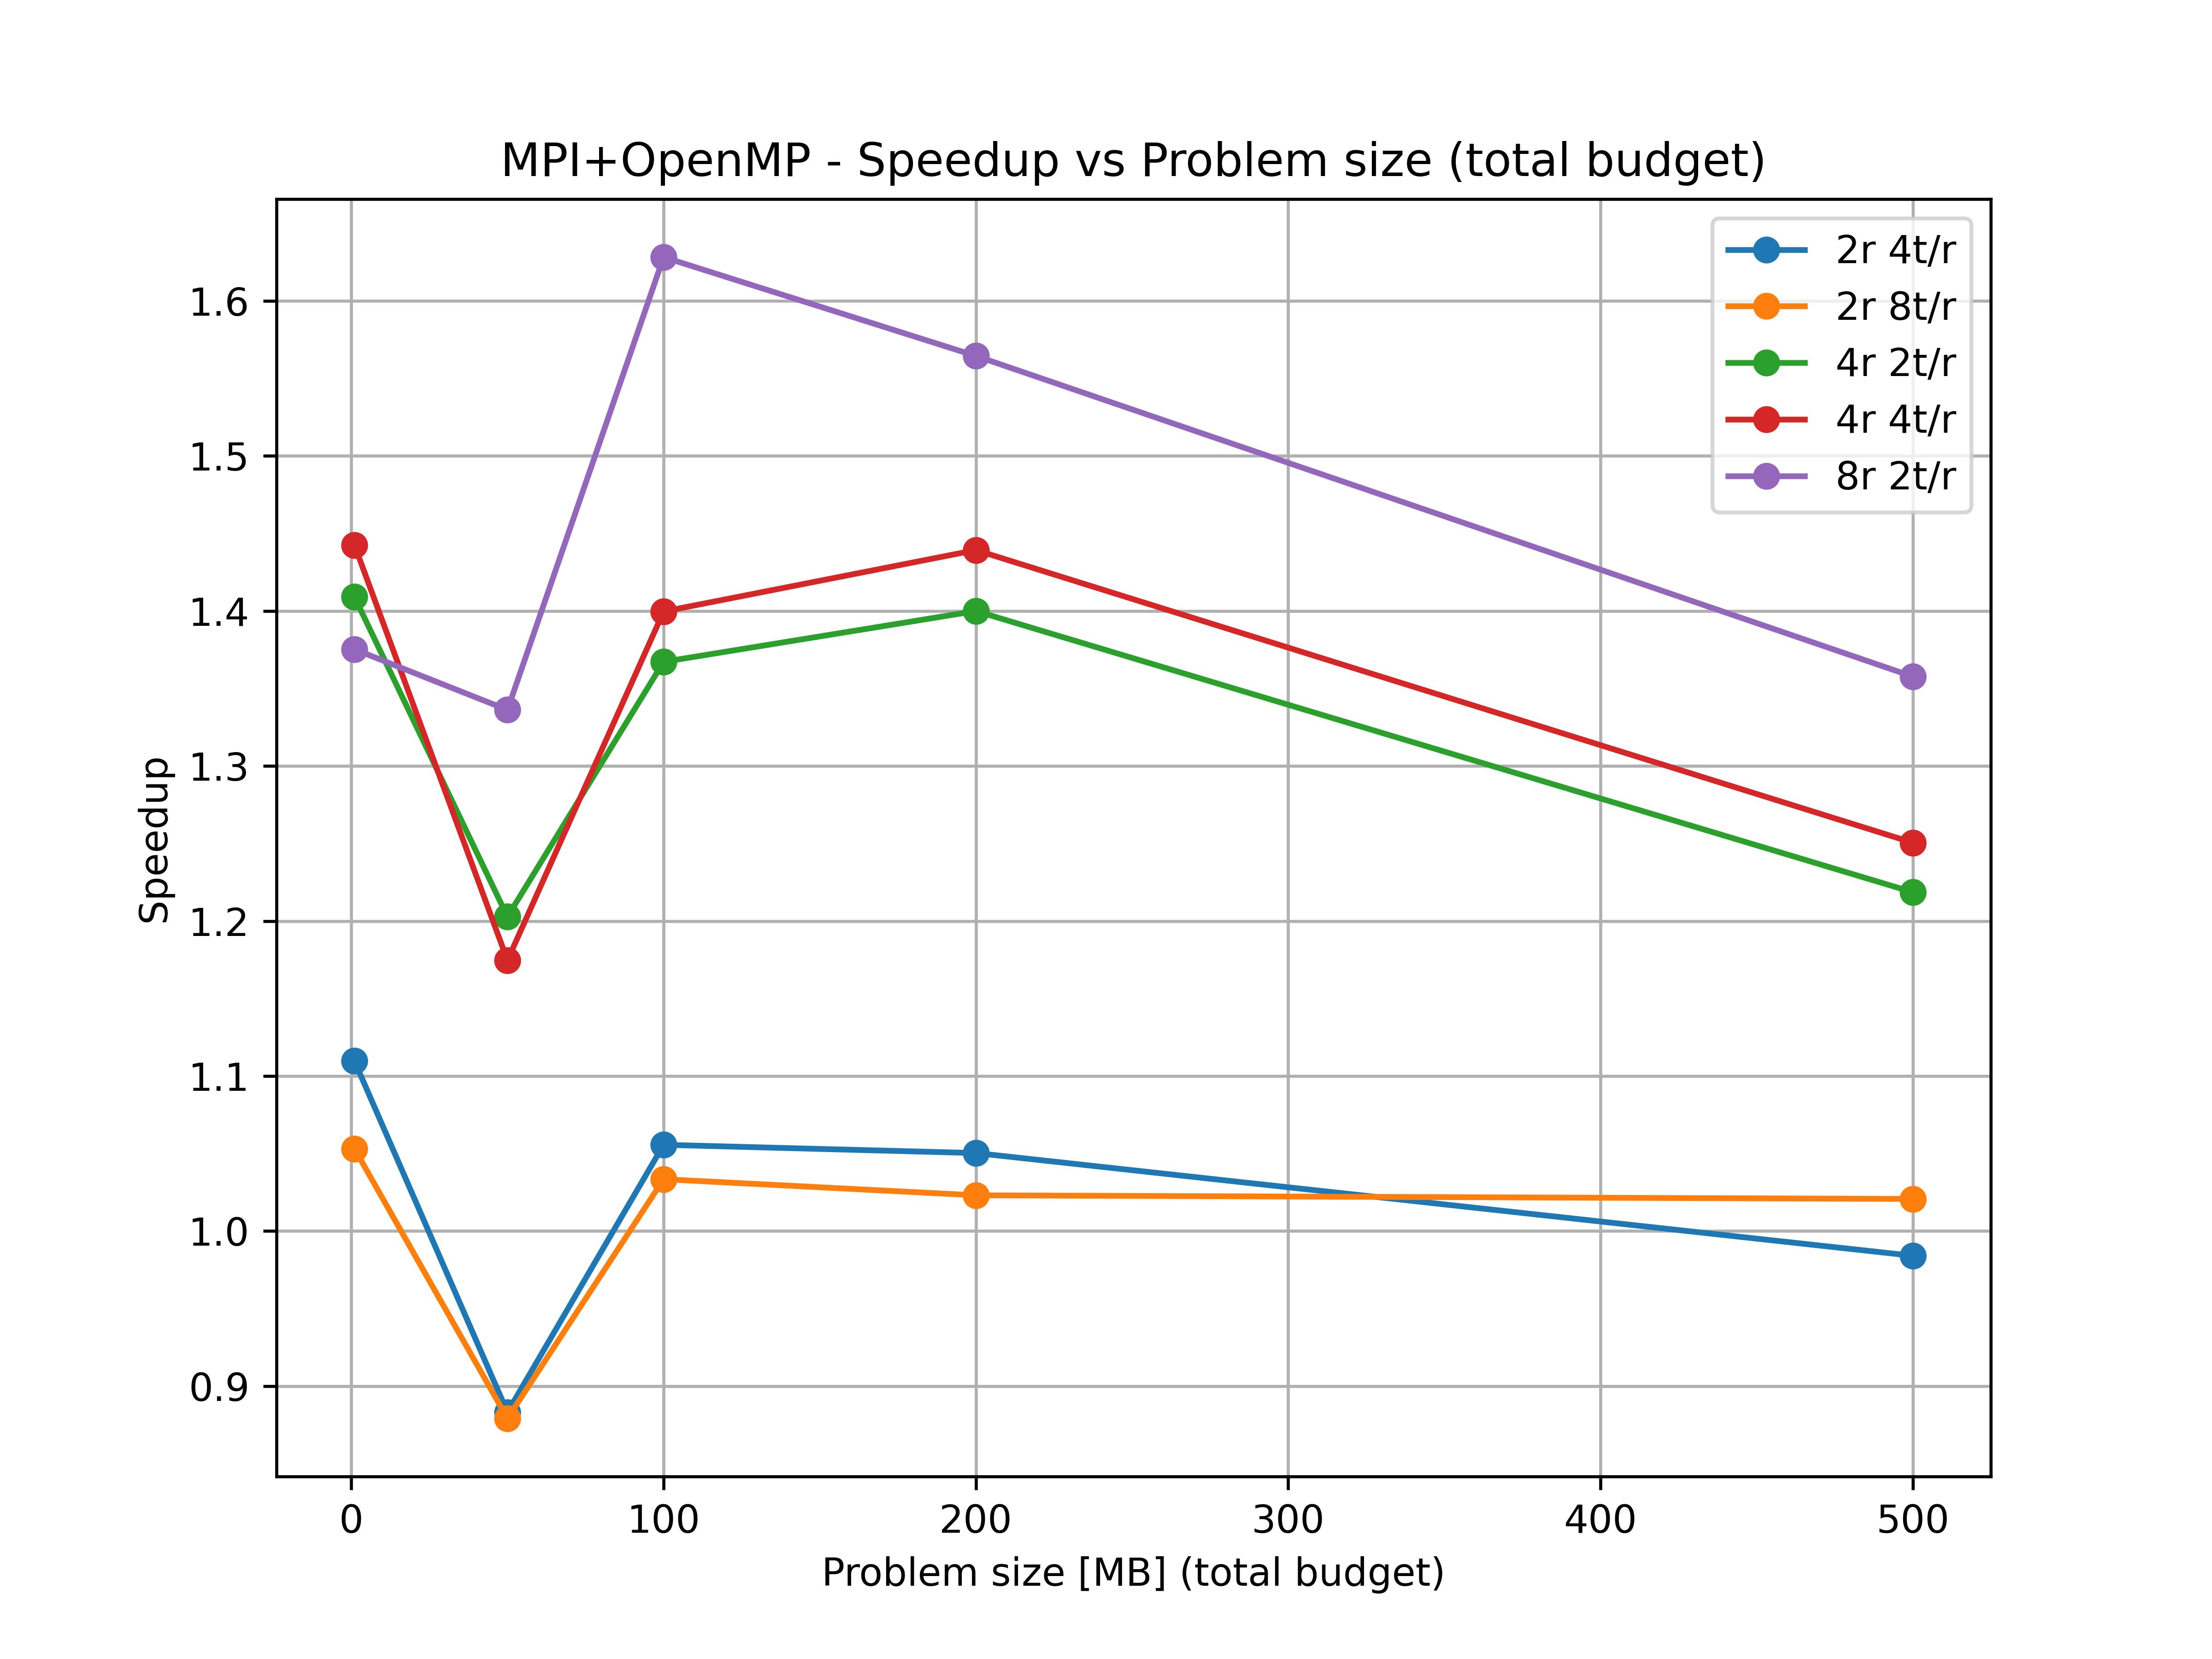
\includegraphics[width=\textwidth]{img/mpi_omp_plots/mpi_omp_speedup.jpg}
					\caption{Speedup MPI+OMP}
					\label{fig:mpi_omp_speedup}
				\end{minipage}
				\hfill
				\begin{minipage}[t]{0.49\textwidth}
					\centering
					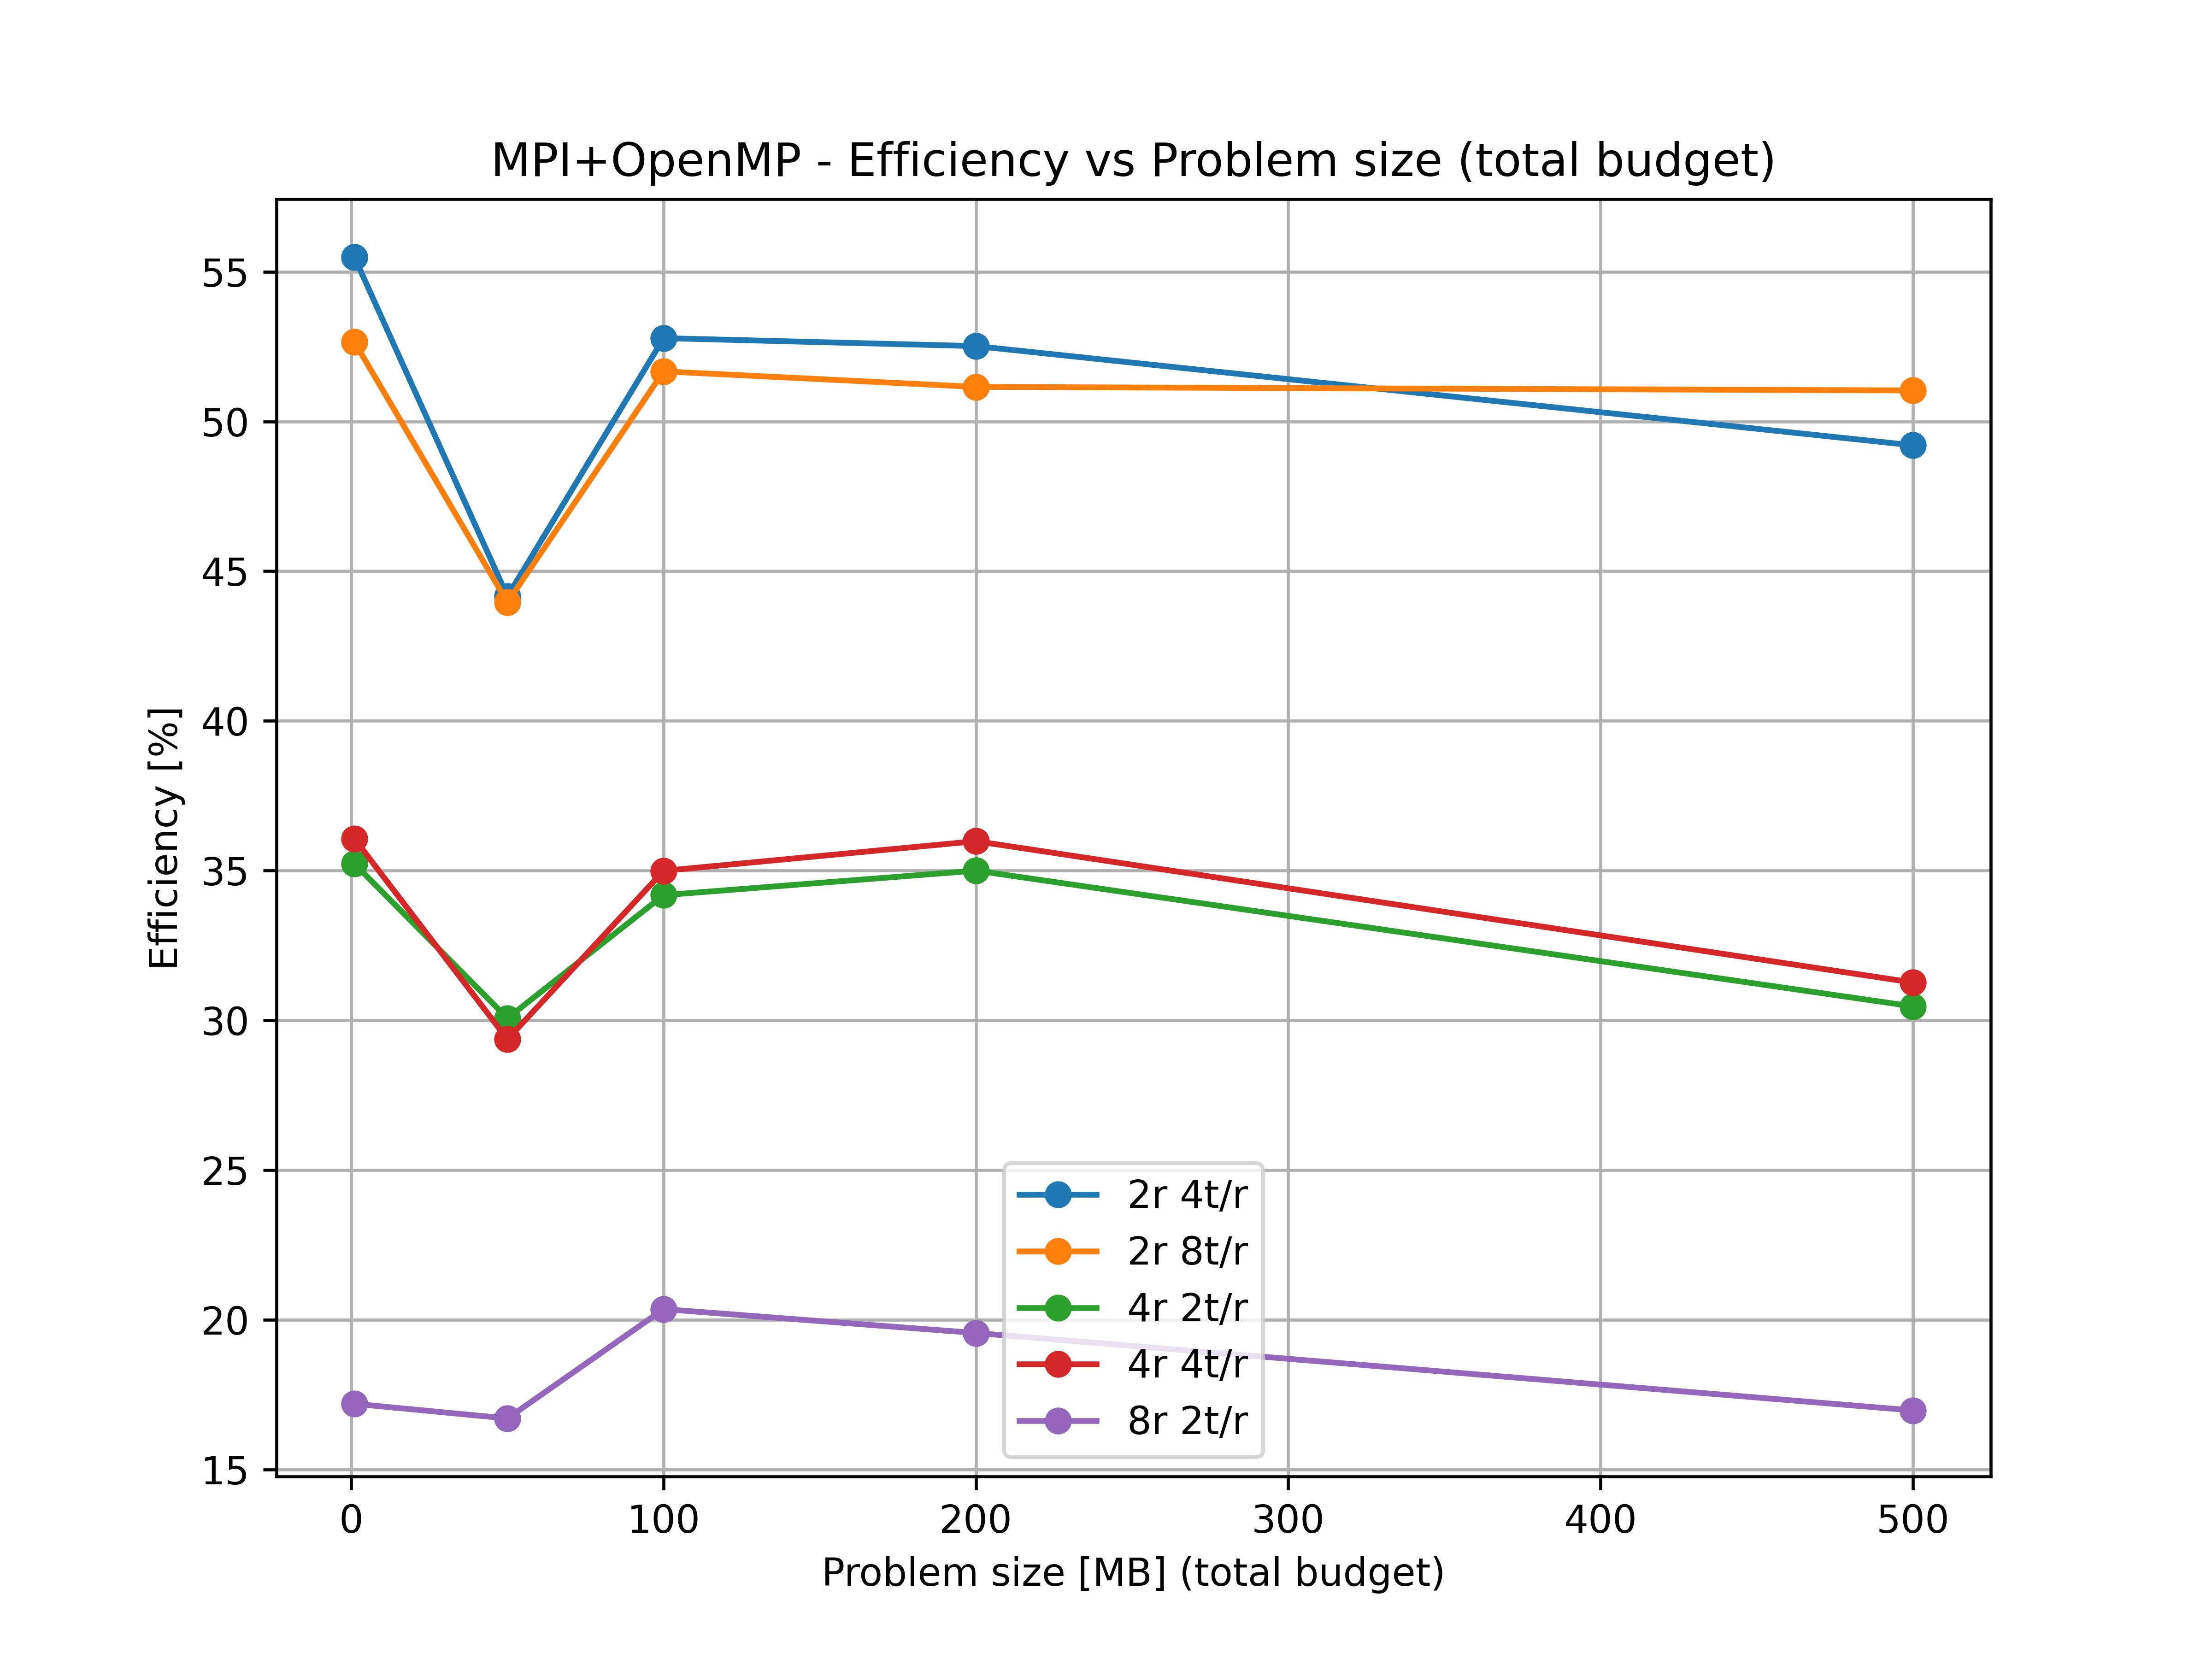
\includegraphics[width=\textwidth]{img/mpi_omp_plots/mpi_omp_efficiency.jpg}
					\caption{Efficiency MPI+OMP}
					\label{fig:mpi_omp_efficiency}
				\end{minipage}
			\end{figure}
			
			\subsubsection*{Osservazioni}
				\begin{itemize}
						\item La configurazione con più ranks e pochi thread (8r$\times$2t) è la più veloce: throughput fino a $\sim$4.6 MB/s e speedup $\sim$1.36$\times$ su 500 MB.
						\item Le configurazioni bilanciate (4r$\times$2t, 4r$\times$4t) ottengono tempi intermedi con efficienze $\sim$30–36\%.
						\item Le configurazioni a 2 ranks (sia 4t che 8t) hanno efficienza più alta (oltre 50\%), ma tempi assoluti peggiori.
						\item L’efficienza cala sistematicamente con l’aumento dei ranks, per via del merge distribuito e della comunicazione.
				\end{itemize}
		
		\subsection{Profiling della memoria}
			Il profiling della memoria è stato condotto su input da 500 MB, strumentando il \emph{rank~0}.
			
			\subsubsection{2 ranks}
				\begin{itemize}
						\item \textbf{2r$\times$4t}: picco $\sim$ \textbf{492 MB}.
						\item \textbf{2r$\times$8t}: picco $\sim$ \textbf{490 MB}.
						\item In entrambi i casi il consumo è simile: array SA/rank da $\sim$100–150 MB ciascuno, buffer \texttt{text} $\sim$50 MB, strutture temporanee di merge.
				\end{itemize}
			
			\subsubsection{4 ranks}
				\begin{itemize}
						\item \textbf{4r$\times$2t}: picco $\sim$ \textbf{460 MB}.
						\item \textbf{4r$\times$4t}: picco $\sim$ \textbf{459 MB}.
						\item La riduzione rispetto a 2 ranks è limitata, poiché rank~0 deve gestire fasi di merge più pesanti.
				\end{itemize}
			
			\subsubsection{8 ranks}
				\begin{itemize}
						\item \textbf{8r$\times$2t}: picco $\sim$ \textbf{333 MB}.
						\item È la configurazione più leggera: la dimensione locale $n_\text{loc}$ ridotta porta a un consumo sensibilmente inferiore.
				\end{itemize}
				
				\begin{figure}[H]
						\centering
						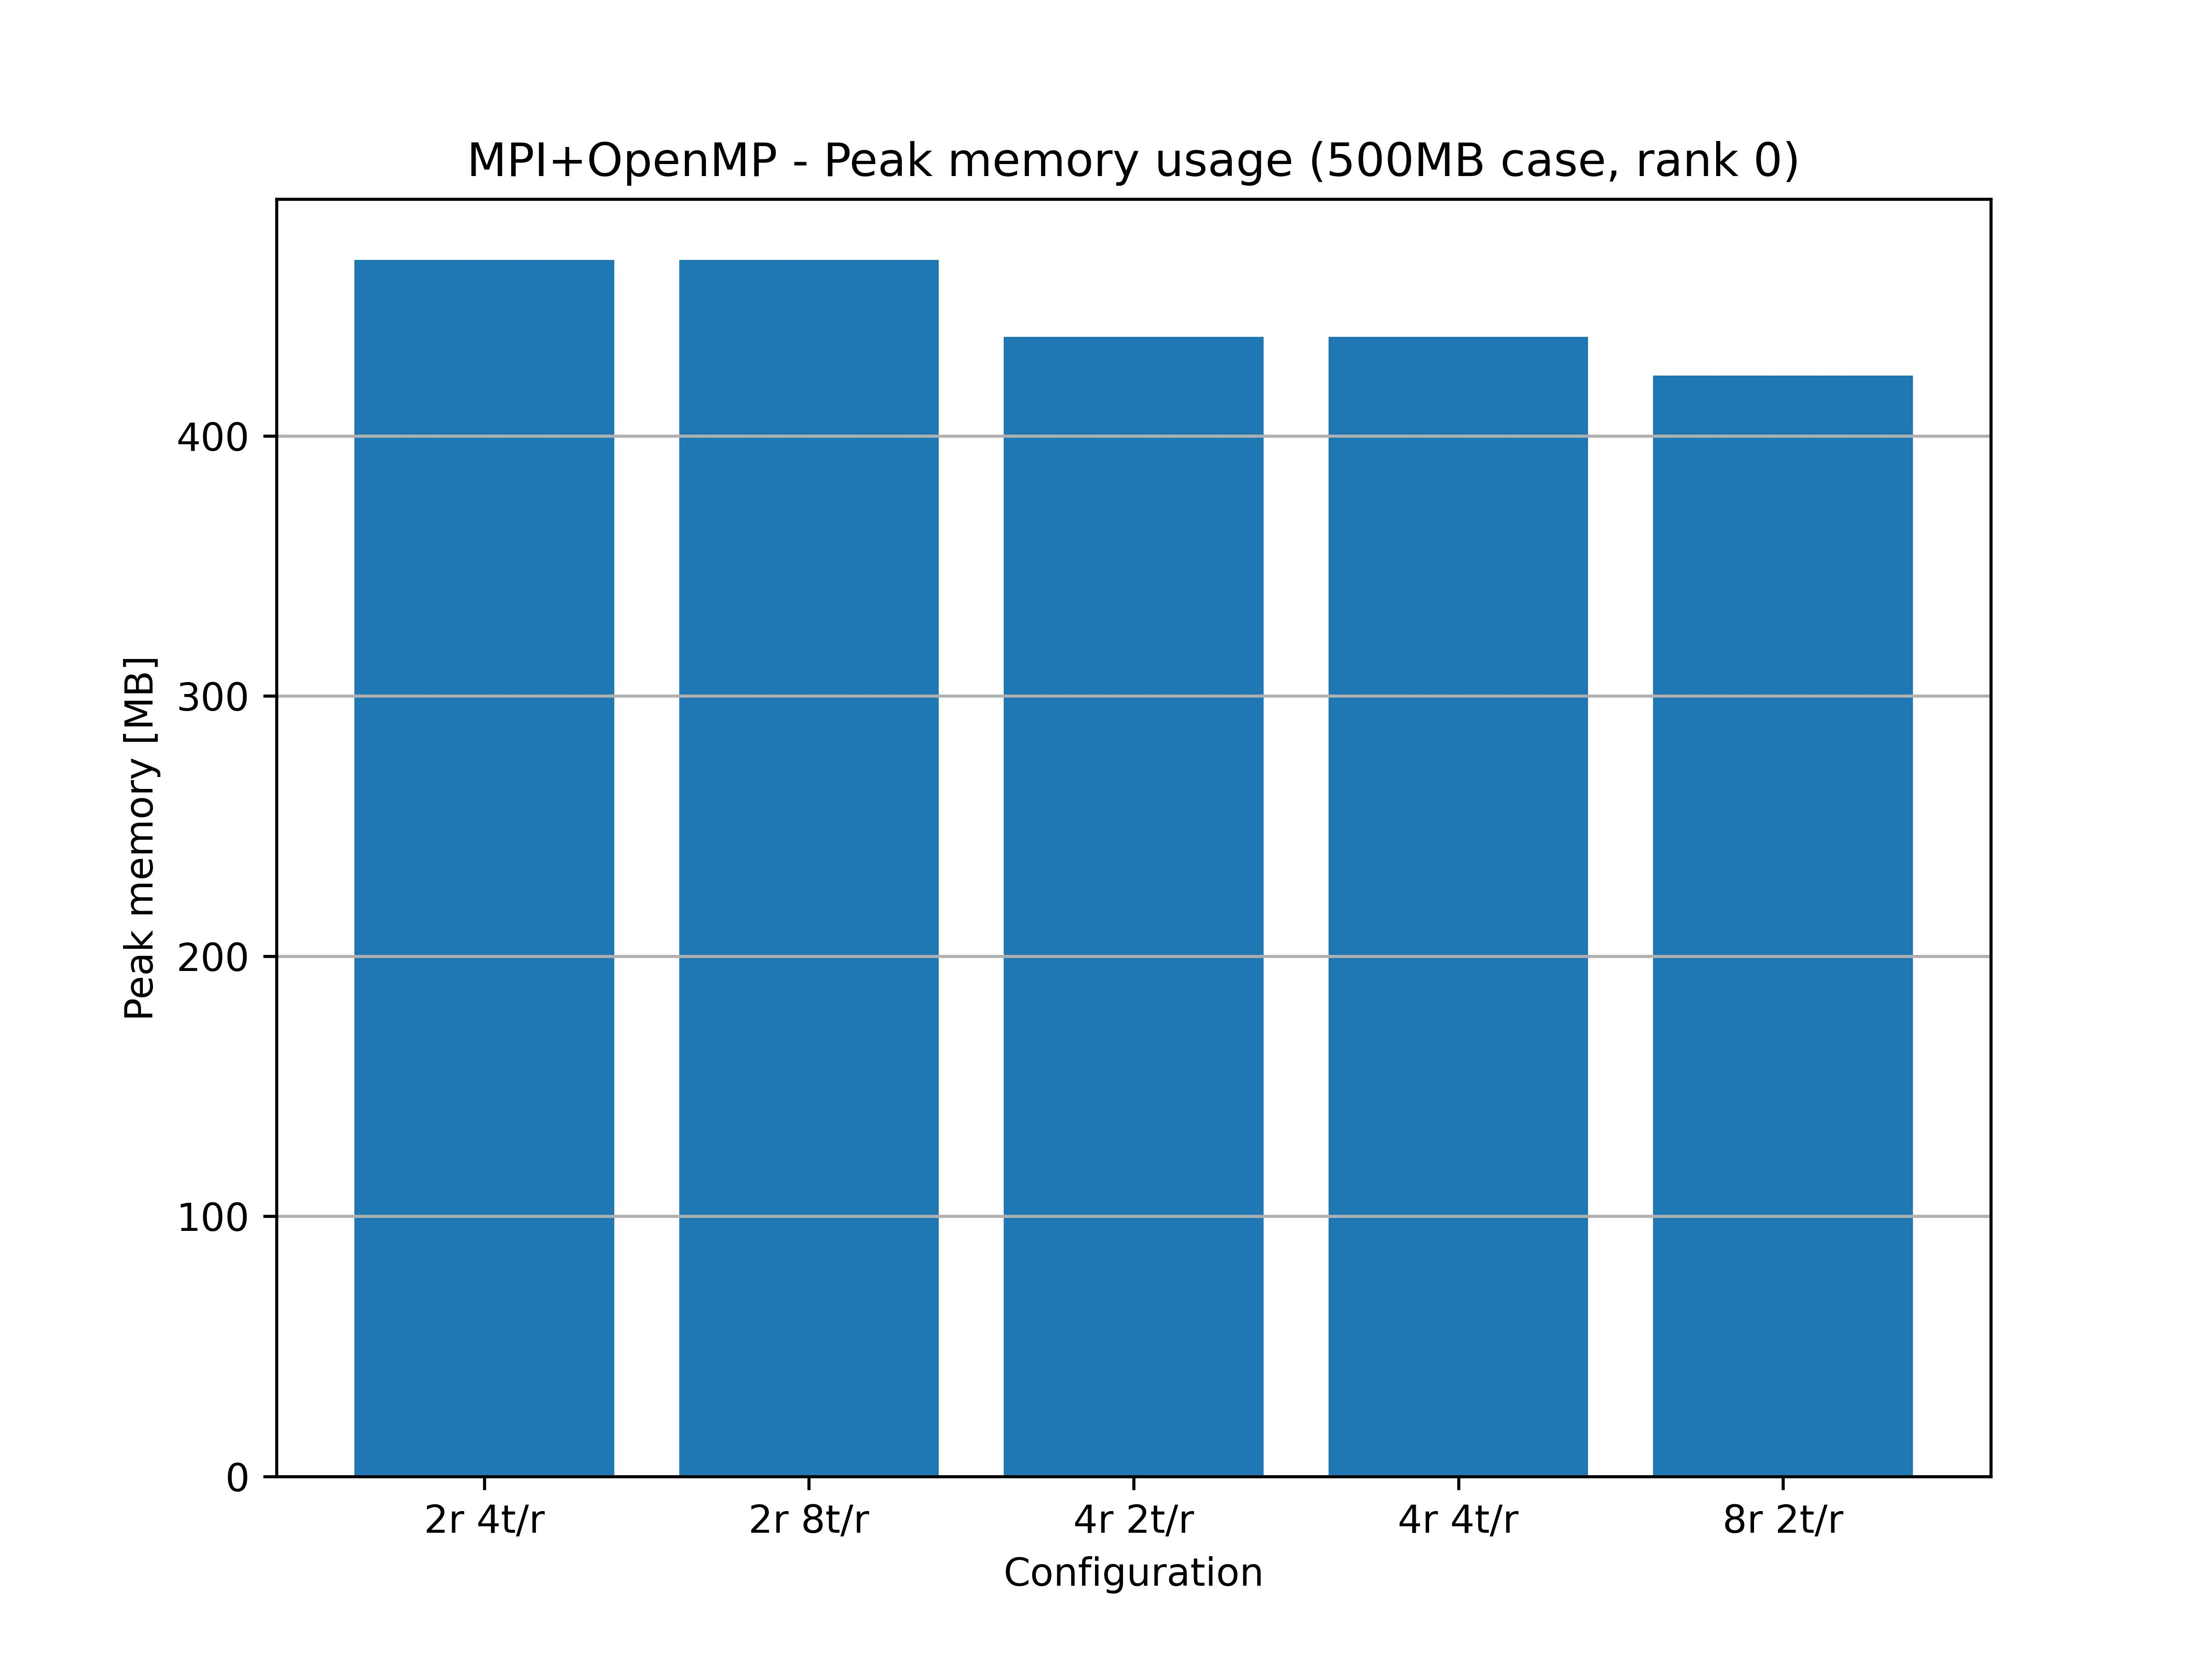
\includegraphics[width=1\linewidth]{img/mpi_omp_plots/mpi_omp_memory.jpg}
						\caption{Memory usage MPI+OMP (rank~0, input 500 MB).}
						\label{fig:mpi_omp_mem_usage}
				\end{figure}
			
			\subsubsection*{Conclusione}
				La memoria scala quasi linearmente con $n_\text{loc}$, scendendo da circa 490 MB (2 ranks) a 333 MB (8 ranks).
				OpenMP non influisce sul footprint, in quanto i thread condividono le strutture dati.
	
	\section{Versione CUDA (single-stream)}
		
		\subsection{Analisi dei tempi}
			I test CUDA (stream singolo) sono stati eseguiti su input da \(\{1,50,100,200,500\}\) MB, 10 run ciascuno, tramite lo script \texttt{cuda\_measure.sh}, che ha prodotto i file \texttt{cuda\_stats.csv} (run grezzi) e \texttt{cuda\_summary.csv} (medie per size).
			La Tabella~\ref{tab:cuda-times} riporta le medie per fase e le metriche aggregate.
			
			\begin{table}[H]
				\centering
				\resizebox{\textwidth}{!}{%
					\begin{tabular}{r r r r r r r r r r r}
						\toprule
						\textbf{Size} & \textbf{Alloc} & \textbf{H2D} & \textbf{Kernel} & \textbf{LCP(CPU)} & \textbf{D2H} &
						\textbf{Compute} & \textbf{Total} & \textbf{Comm} & \textbf{MB/s} & \textbf{Speedup / Eff.} \\
						\textbf{(MB)} & \textbf{(s)} & \textbf{(s)} & \textbf{(s)} & \textbf{(s)} & \textbf{(s)} &
						\textbf{pure (s)} & \textbf{compute (s)} & \textbf{(s)} &  & \textbf{(\(\times\) / \%)} \\
						\midrule
						1   & 0.1153 & 0.00002 & 0.0040 & 0.00045 & 0.00016 & 0.00447 & 0.1198 & 0.00018 & 10.67 & 1.30 / 129.7 \\
						50  & 0.1098 & 0.00030 & 0.0741 & 0.0584  & 0.00572 & 0.1325  & 0.2422 & 0.00602 & 17.99 & 2.95 / 294.9 \\
						100 & 0.1014 & 0.00066 & 0.1468 & 0.1545  & 0.01111 & 0.3013  & 0.4027 & 0.01176 & 15.81 & 3.34 / 334.4 \\
						200 & 0.1001 & 0.00142 & 0.3132 & 0.3746  & 0.02208 & 0.6878  & 0.7879 & 0.02350 & 13.85 & 3.37 / 337.0 \\
						500 & 0.1013 & 0.00366 & 0.8466 & 1.1234  & 0.05524 & 1.9700  & 2.0712 & 0.05891 & 12.09 & 3.56 / 355.7 \\
						\bottomrule
					\end{tabular}}
				\caption{CUDA single-stream — Medie (10 run) per dimensione: tempi per fase, throughput e speedup/efficienza.}
				\label{tab:cuda-times}
			\end{table}
			
			\begin{figure}[H]
				\centering
				\begin{minipage}[t]{0.49\textwidth}
					\centering
					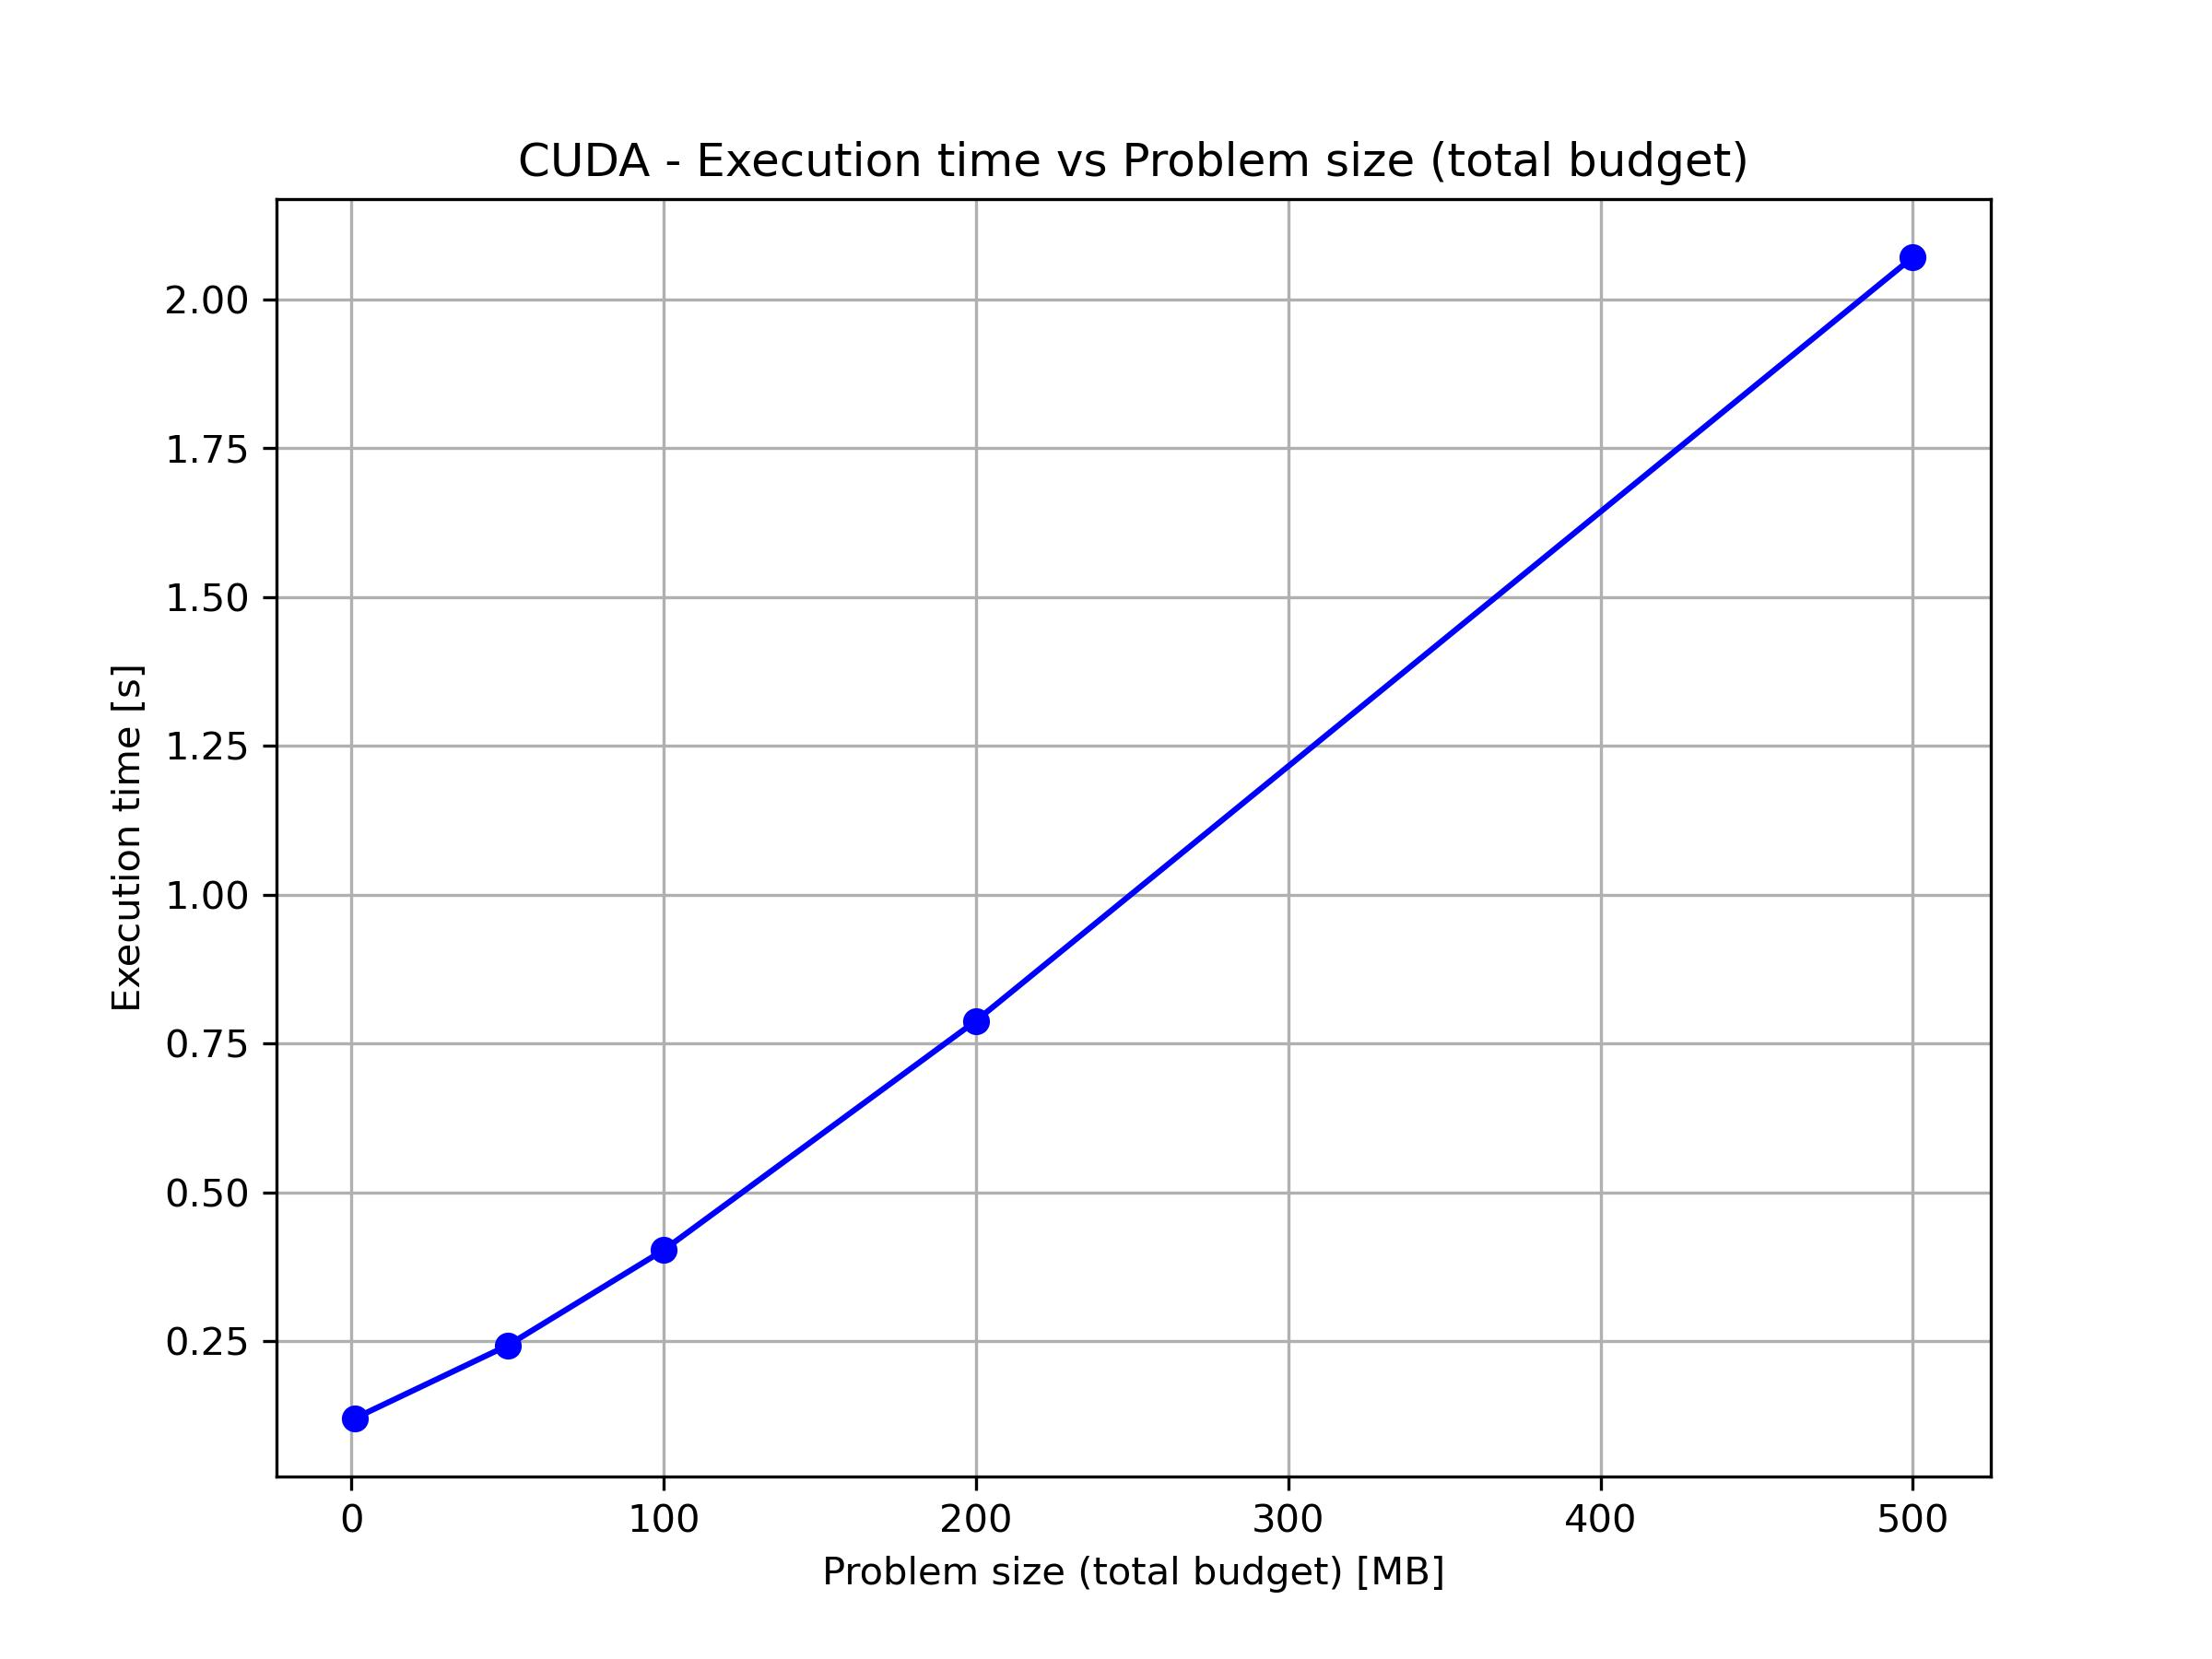
\includegraphics[width=\textwidth]{img/cuda_plots/cuda_times.jpg}
					\caption{Tempi CUDA}
					\label{fig:cuda_times}
				\end{minipage}
				\hfill
				\begin{minipage}[t]{0.49\textwidth}
					\centering
					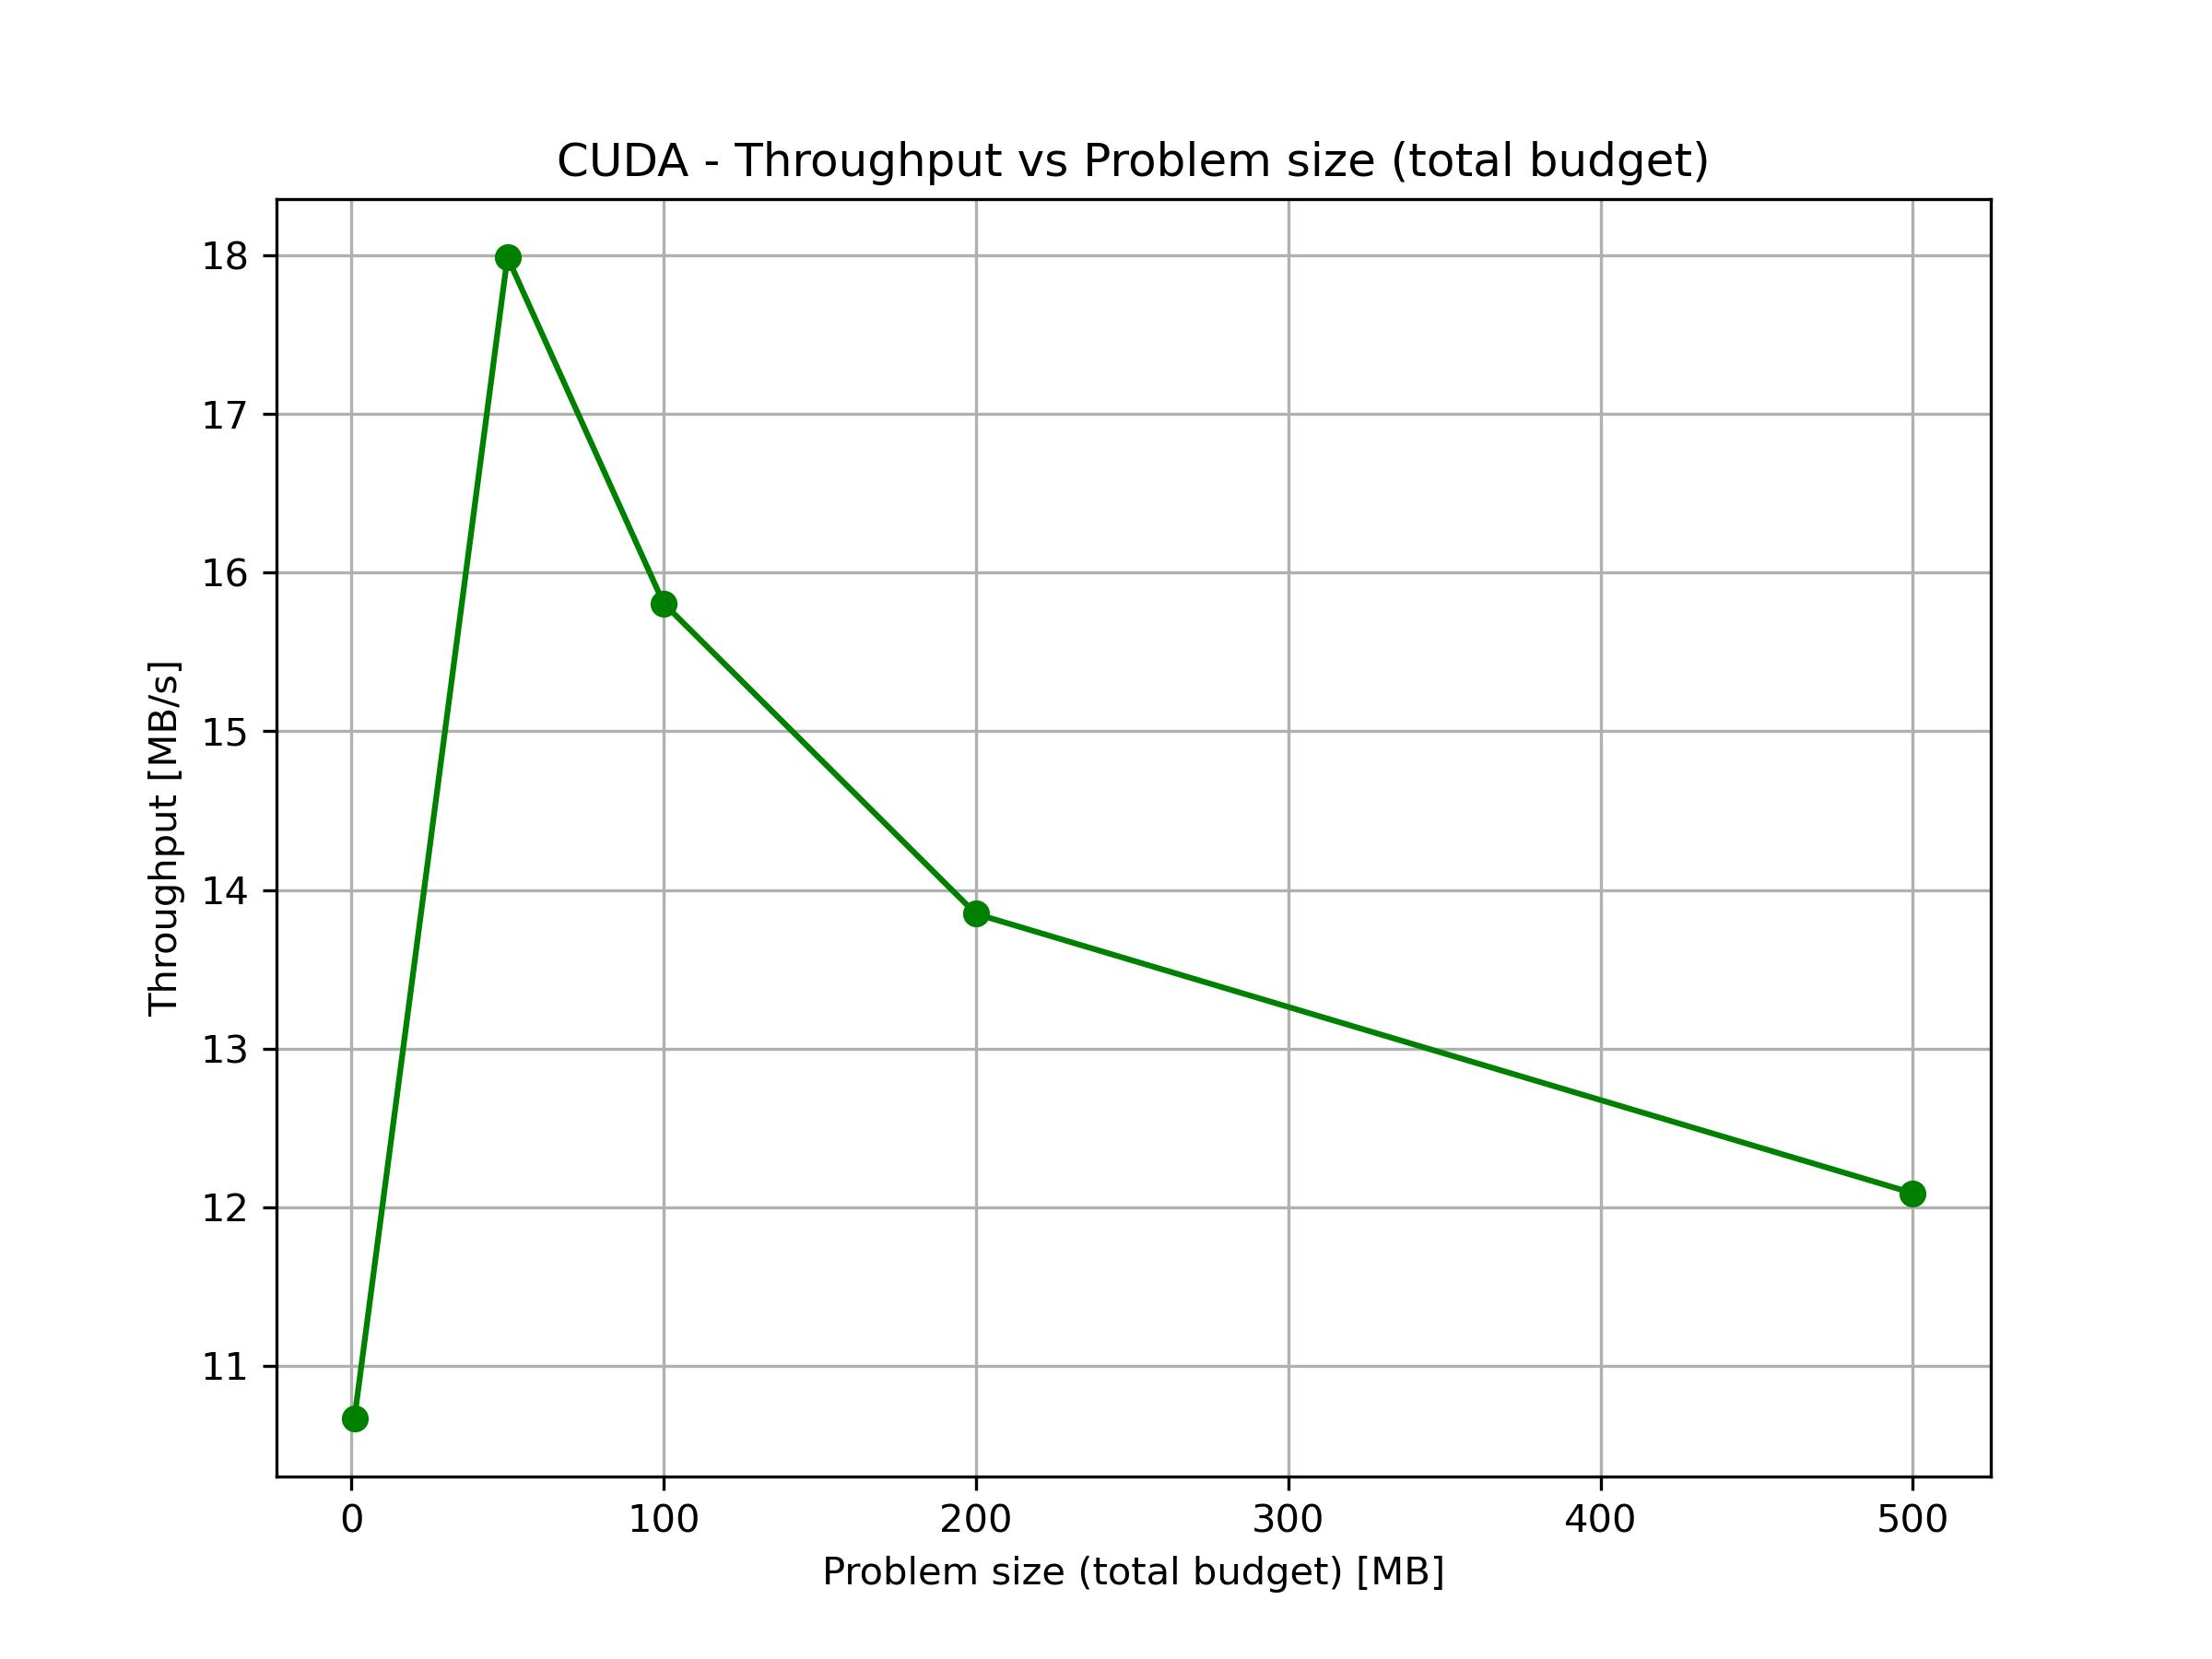
\includegraphics[width=\textwidth]{img/cuda_plots/cuda_throughput.jpg}
					\caption{Throughput CUDA}
					\label{fig:cuda_throughput}
				\end{minipage}
			\end{figure}
			
			\begin{figure}[H]
				\centering
				\begin{minipage}[t]{0.49\textwidth}
					\centering
					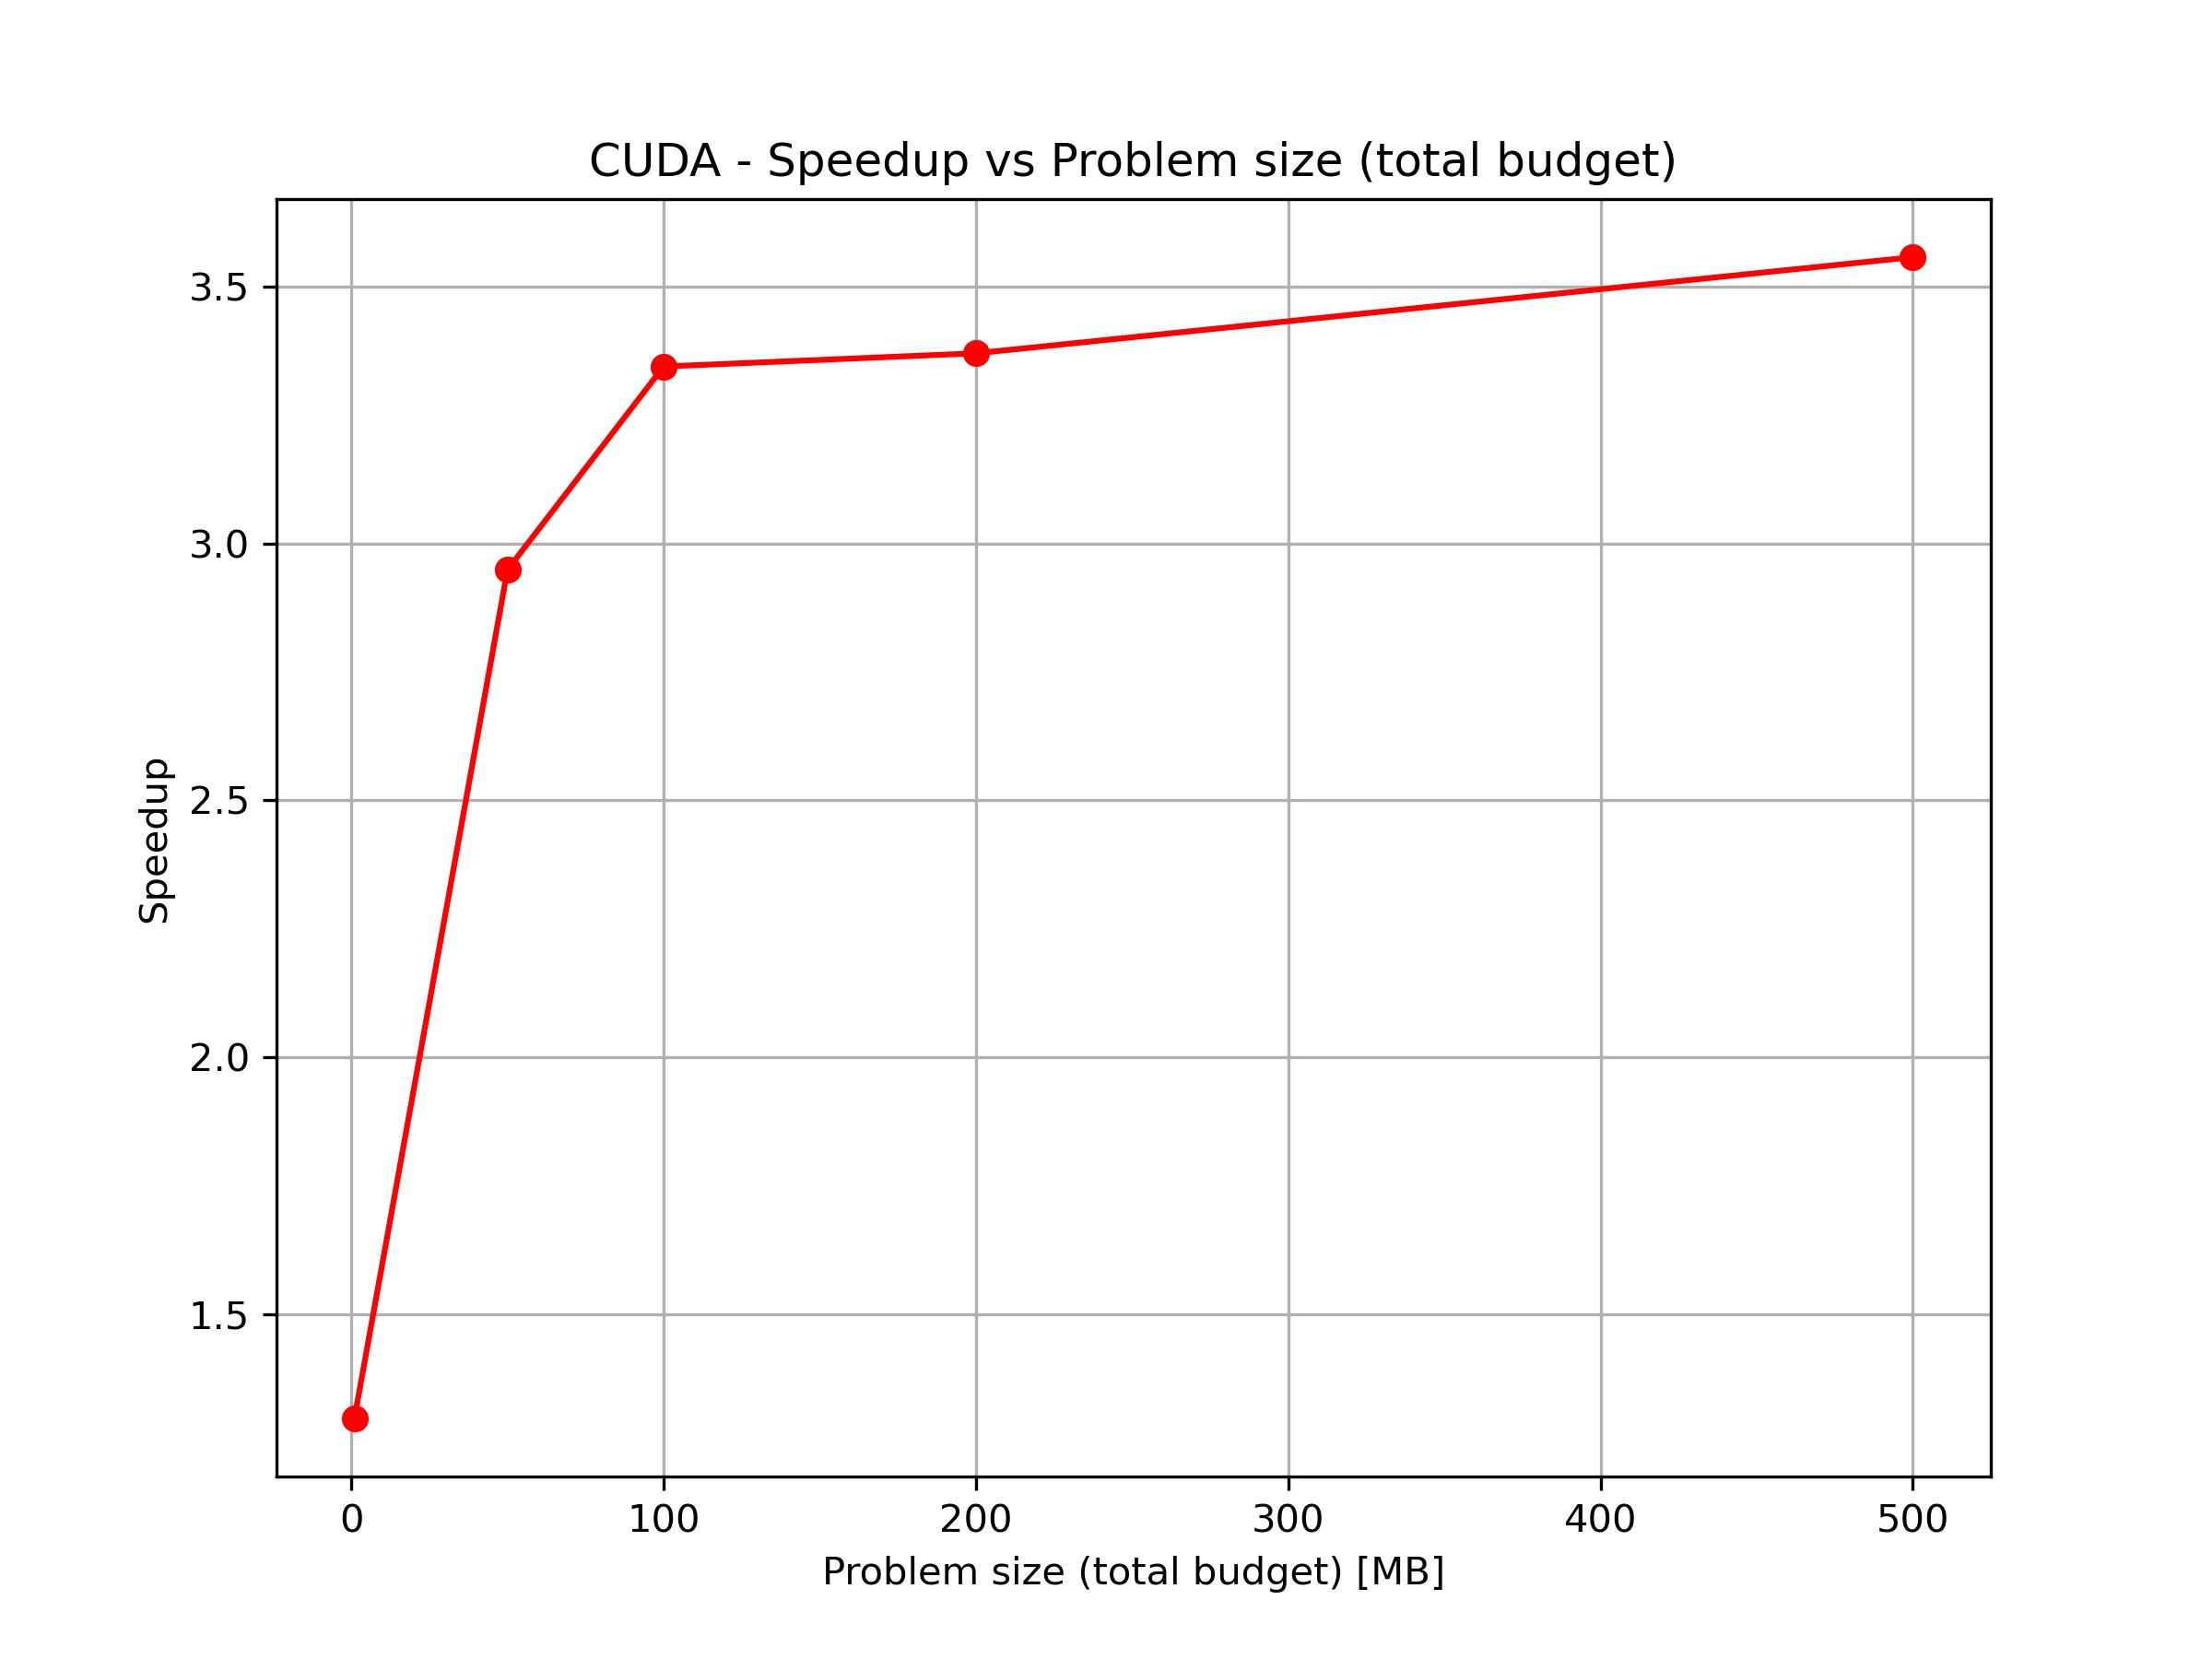
\includegraphics[width=\textwidth]{img/cuda_plots/cuda_speedup.jpg}
					\caption{Speedup CUDA}
					\label{fig:cuda_speedup}
				\end{minipage}
				\hfill
				\begin{minipage}[t]{0.49\textwidth}
					\centering
					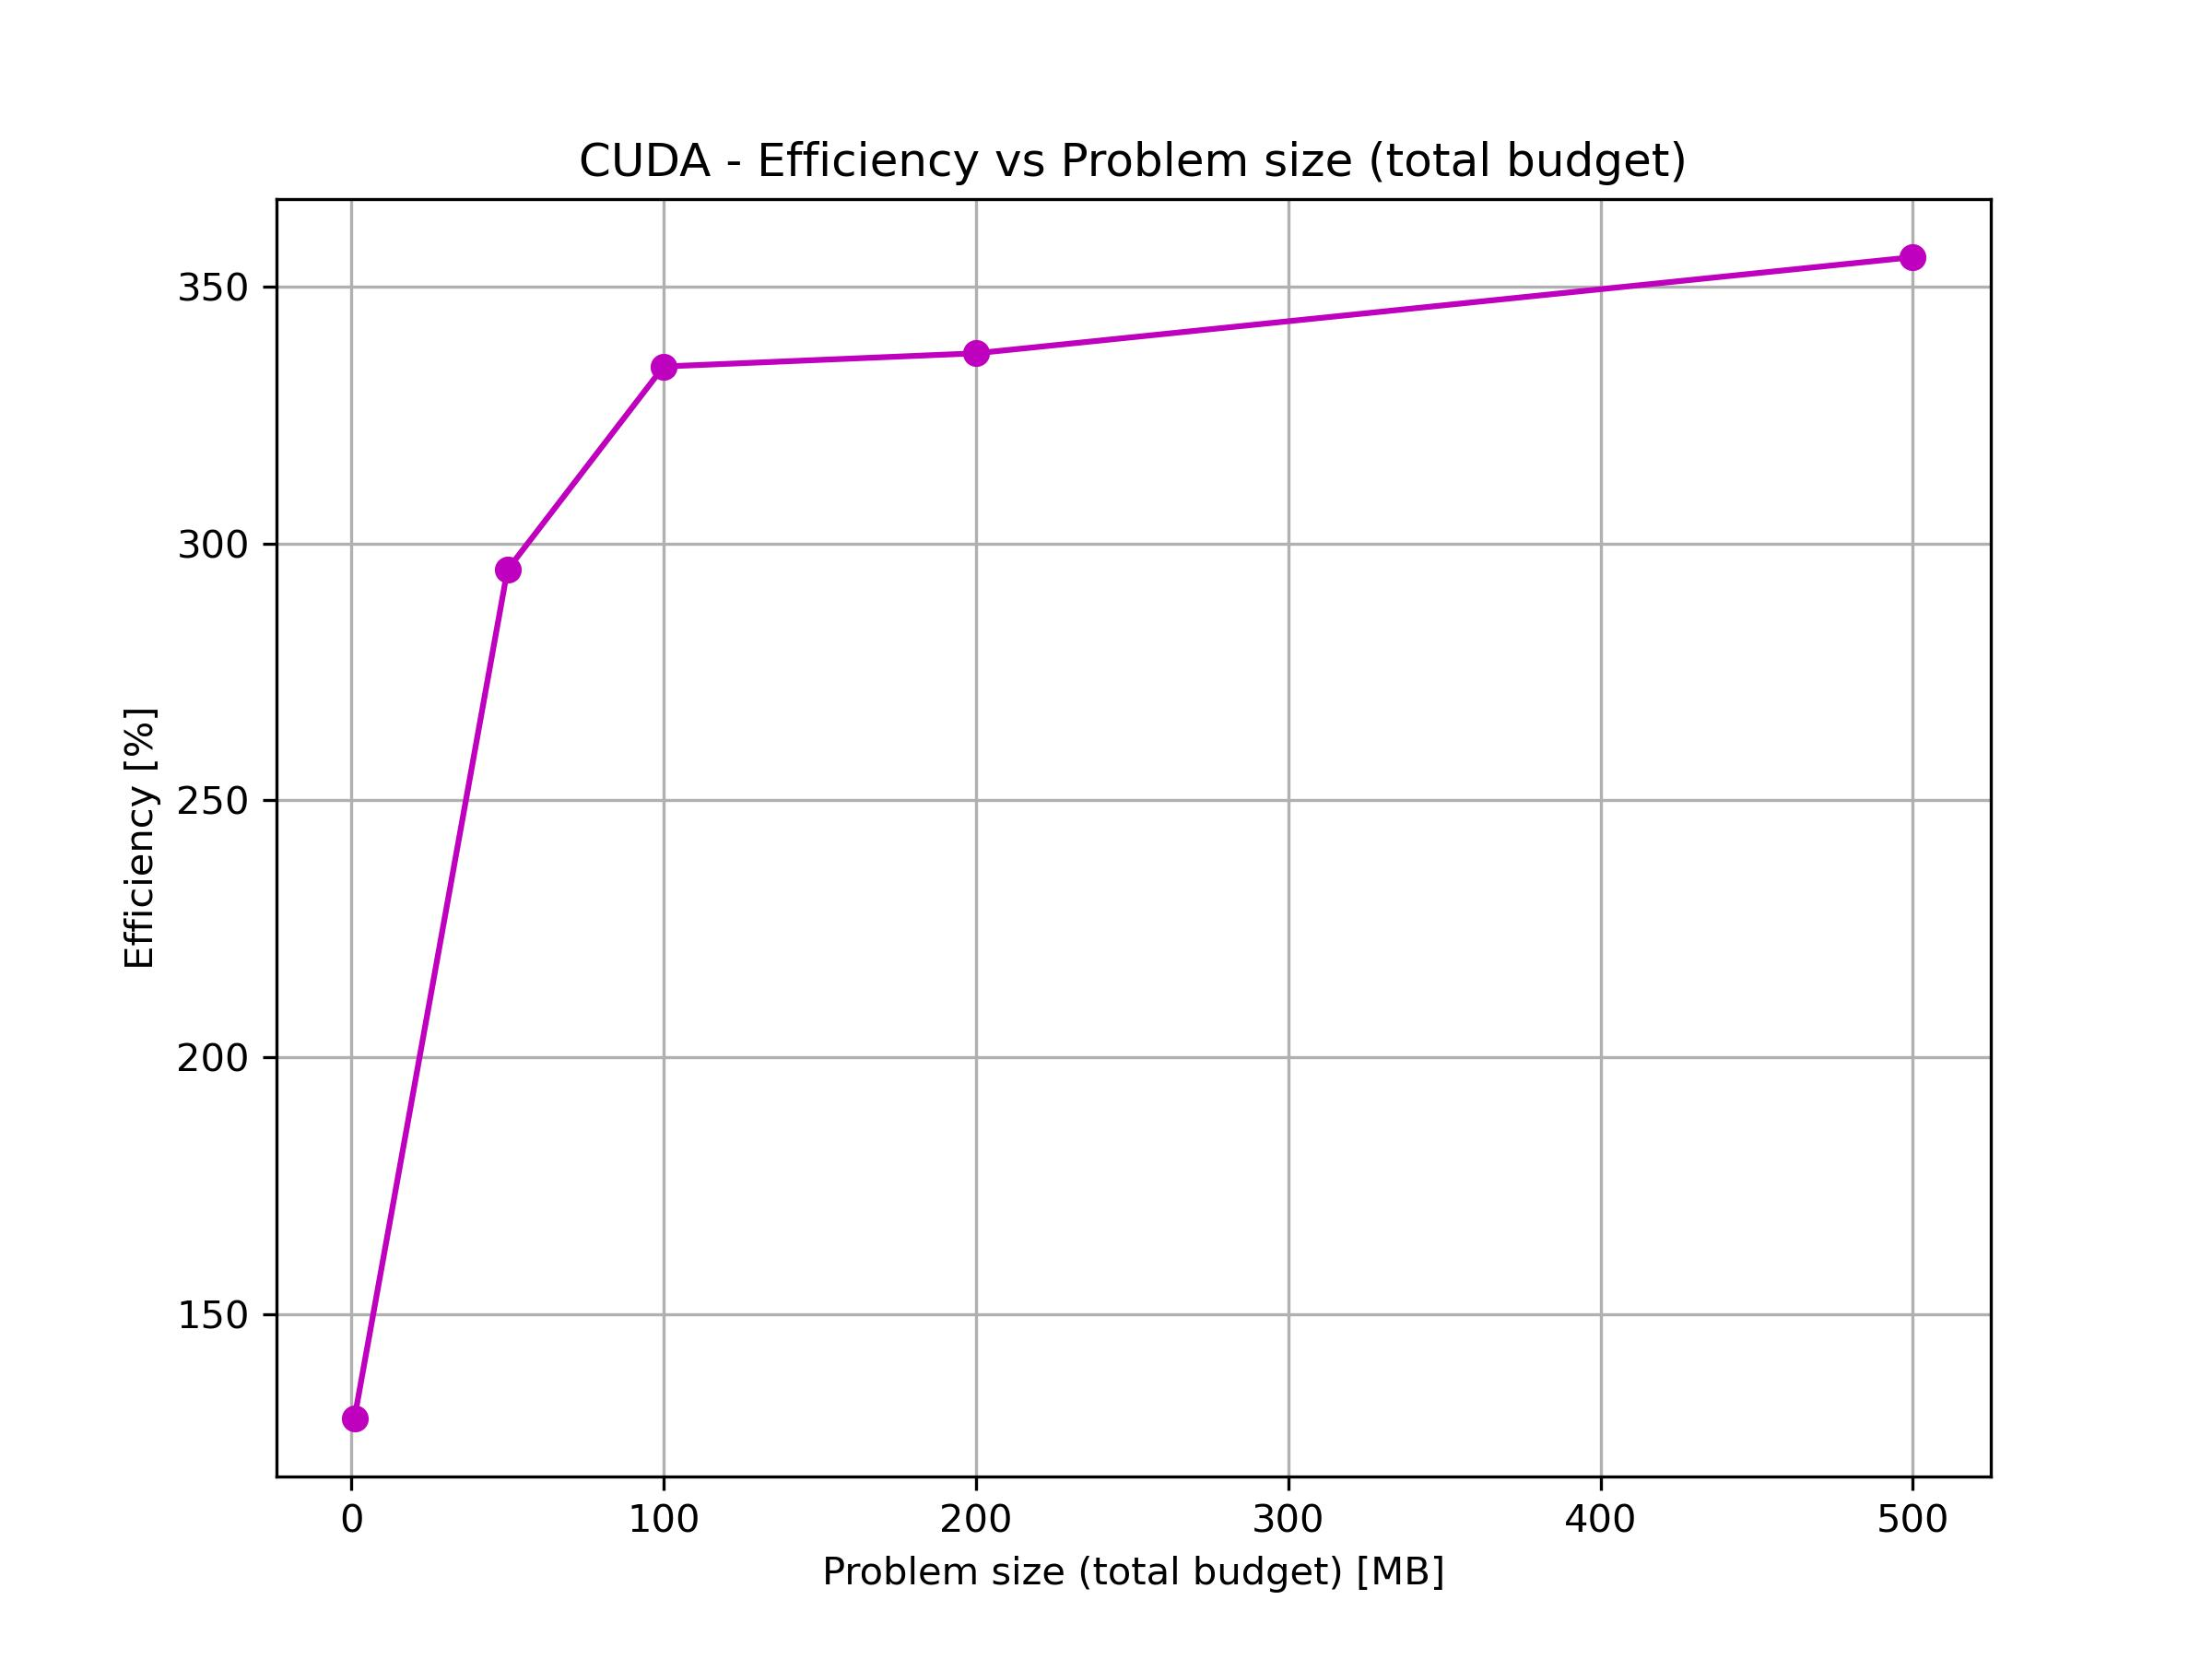
\includegraphics[width=\textwidth]{img/cuda_plots/cuda_efficiency.jpg}
					\caption{Efficiency CUDA}
					\label{fig:cuda_efficiency}
				\end{minipage}
			\end{figure}
			
			\subsubsection*{Osservazioni}
				\begin{itemize}
						\item Il tempo è dominato dal \textbf{kernel GPU} e dalla \textbf{costruzione LCP su CPU}: a 500 MB il kernel impiega \(\sim 0.85\) s (\(\sim 43\%\)) e LCP \(\sim 1.12\) s (\(\sim 54\%\)).
						\item Le \textbf{transfer} (\(\text{H2D}+\text{D2H}\)) restano marginali: \(\sim 0.06\) s su 2.07 s totali (\(<3\%\)).
						\item Il \textbf{throughput} cala con l’aumento della dimensione: da \(\sim 18\) MB/s (50 MB) a \(\sim 12\) MB/s (500 MB).
						\item Lo \textbf{speedup} medio rispetto al sequenziale è \(\sim 3.3{-}3.6\times\) per input grandi.
				\end{itemize}
		
		\subsection{Profiling della memoria}
			Il profilo a 500 MB è stato approfondito con \texttt{ncu} (\textit{Nsight Compute}) usando \texttt{ncu\_cuda\_profile.sh}.
			Nel run profilato (\texttt{cuda\_500MB\_profile.txt/.ncu-rep}) si osservano:
			\begin{itemize}
				\item \texttt{time\_kernel\_gpu} \(\approx 0.857\) s,
				\item \texttt{time\_lcp\_cpu} \(\approx 1.106\) s,
				\item \texttt{time\_h2d} \(\approx 0.004\) s, \texttt{time\_d2h} \(\approx 0.055\) s \(\Rightarrow\) transfer complessive \(\sim 0.06\) s (\(\sim 2.8\%\) del compute),
				\item \texttt{time\_alloc\_host\_dev}: \(\sim 0.10\) s nelle medie, ma fino a \(>2\) s con \texttt{ncu} per effetto dell’overhead dello strumento.
			\end{itemize}
			
			\subsubsection*{Footprint in memoria}
				Nel caso single-stream, il footprint è dato da:
				\begin{enumerate}
						\item \textbf{Buffer del testo} su device (\(\sim n\) byte) e relativa copia host (pinned).
						\item \textbf{Array ausiliari} per il SA/LRS su GPU (\(O(n)\) interi a 32 bit).
						\item \textbf{Strutture LCP su CPU} (\(O(n)\) interi) per la \emph{Kasai} finale.
				\end{enumerate}
				Il rapporto \texttt{memory\_overhead\_ratio} decresce con l’input: da \(\sim 96\%\) (1 MB, dominato da overhead fissi) a \(\sim 8\%\) (500 MB).
				
				\begin{figure}[H]
						\centering
						\begin{minipage}[t]{0.49\textwidth}
							\centering
							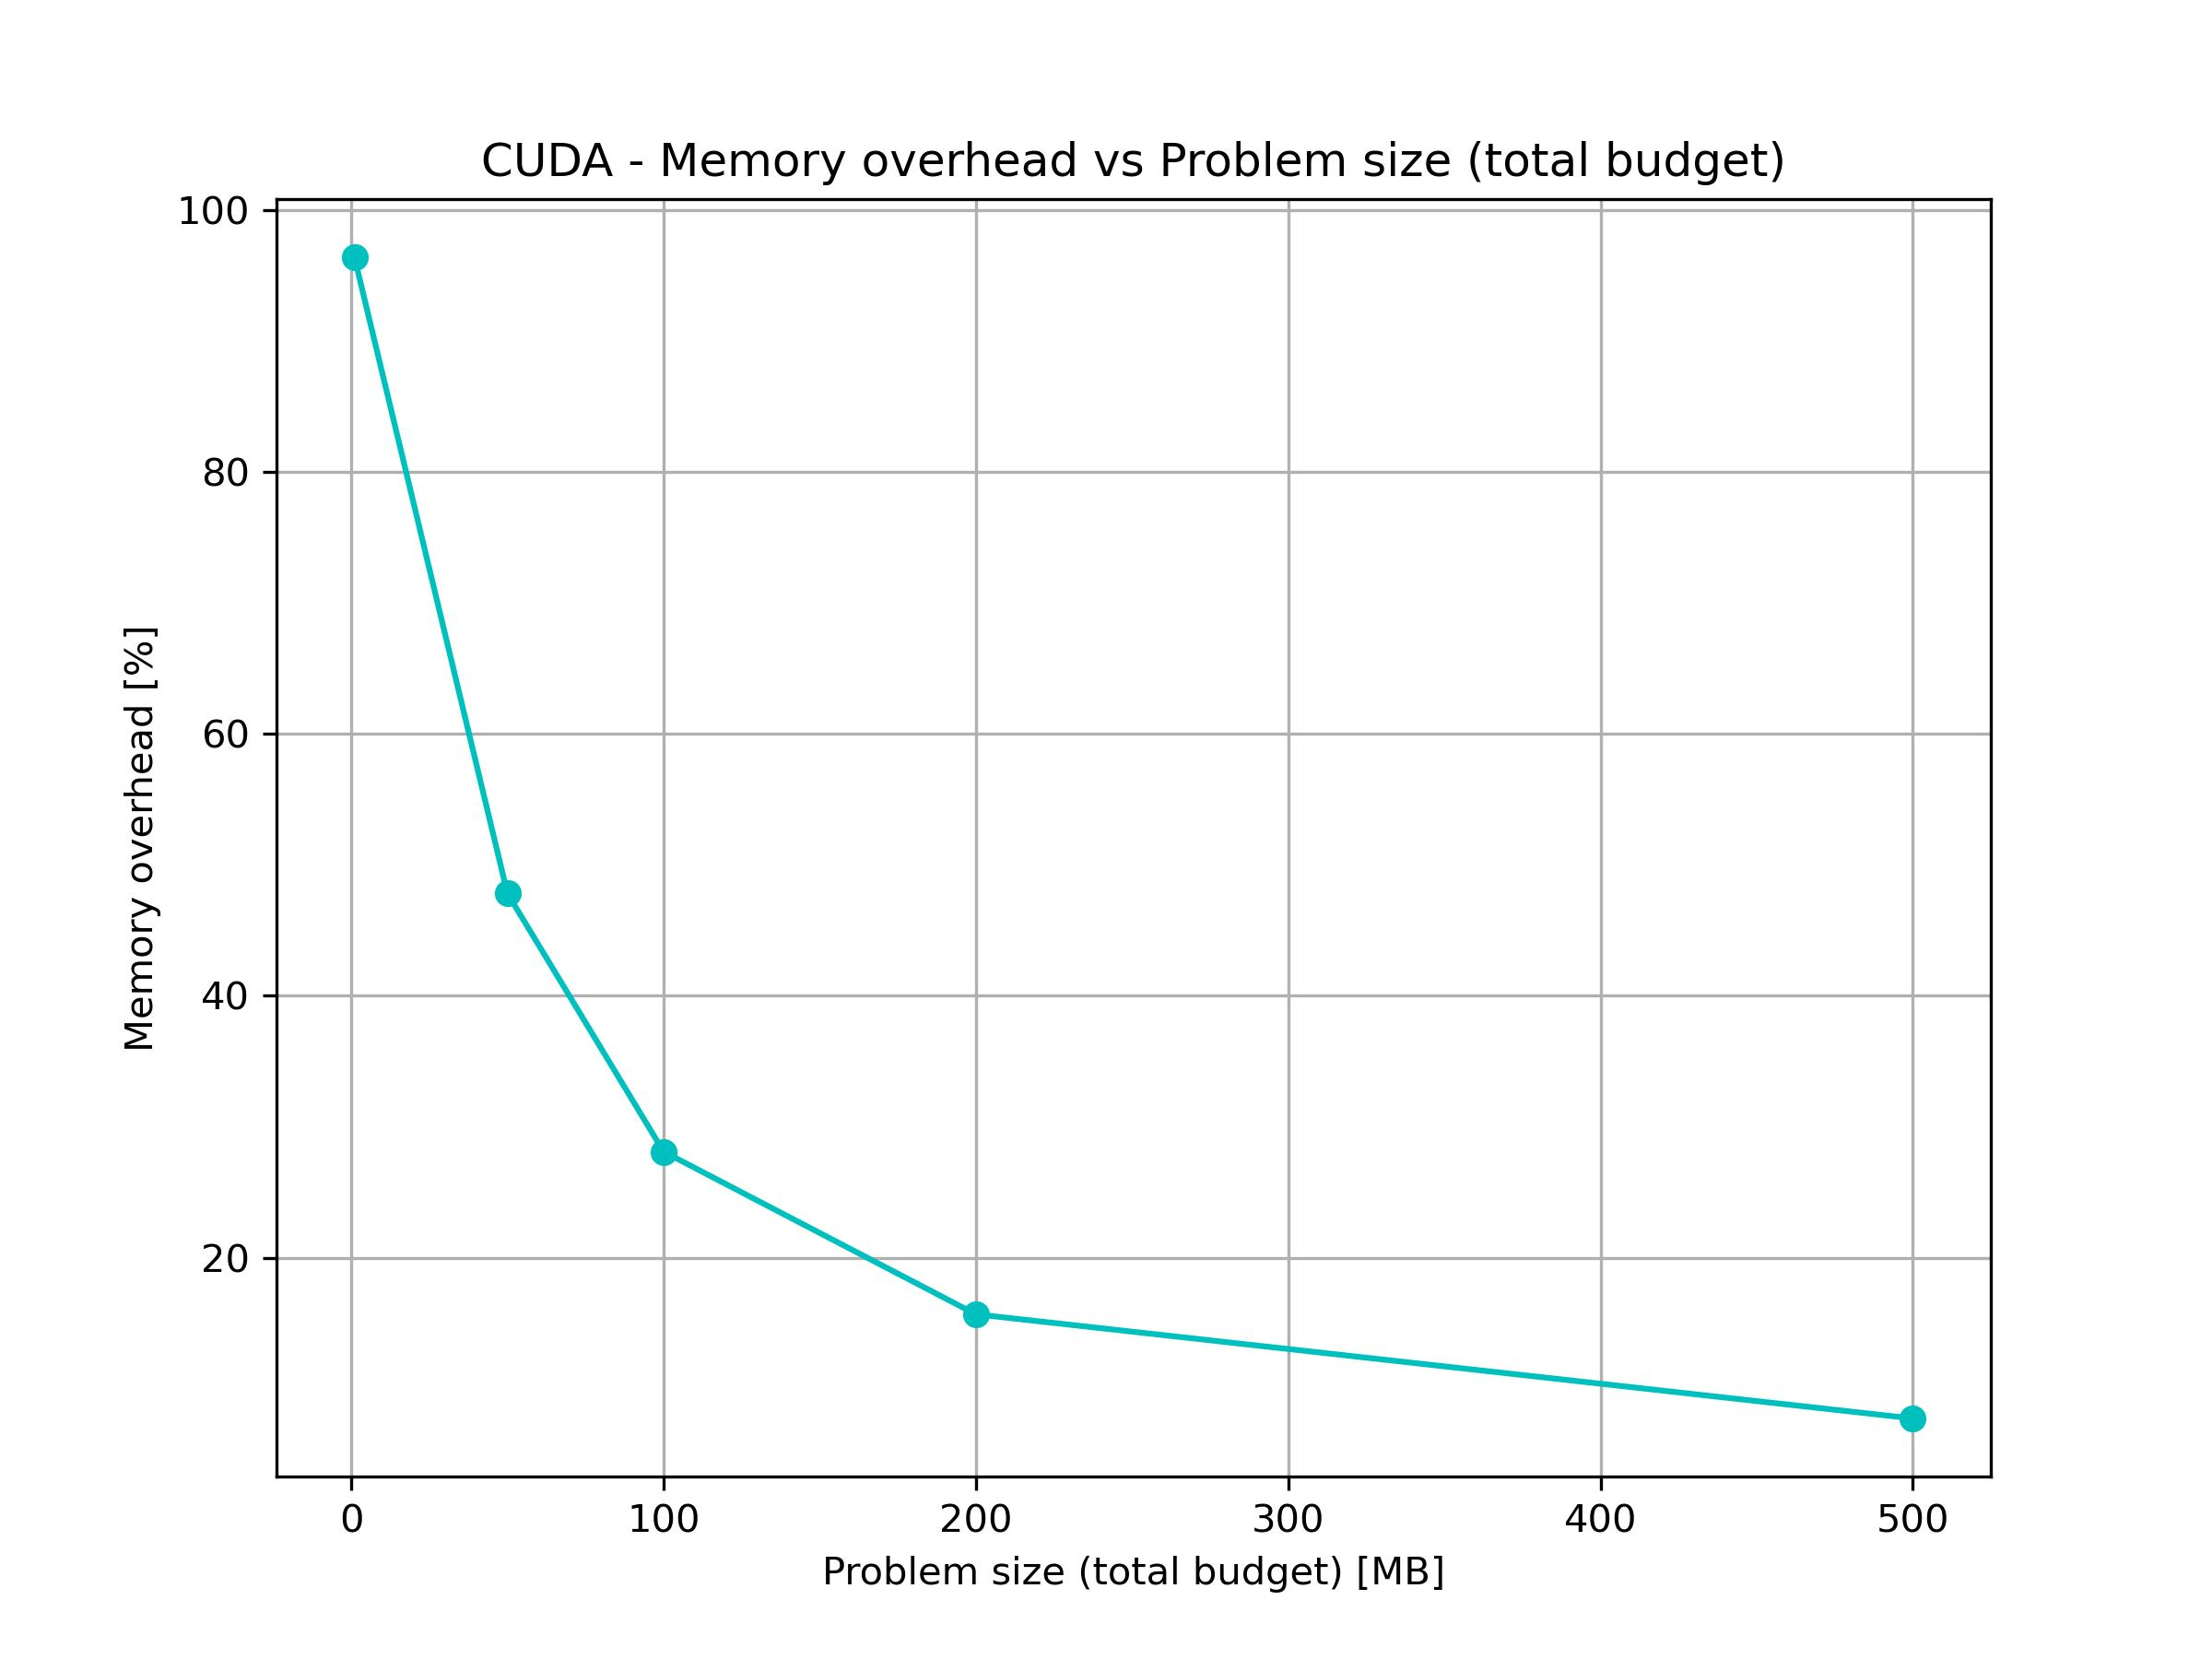
\includegraphics[width=\textwidth]{img/cuda_plots/cuda_memory_overhead.jpg}
							\caption{Memory overhead CUDA}
							\label{fig:cuda_mem_overhead}
						\end{minipage}
						\hfill
						\begin{minipage}[t]{0.49\textwidth}
							\centering
							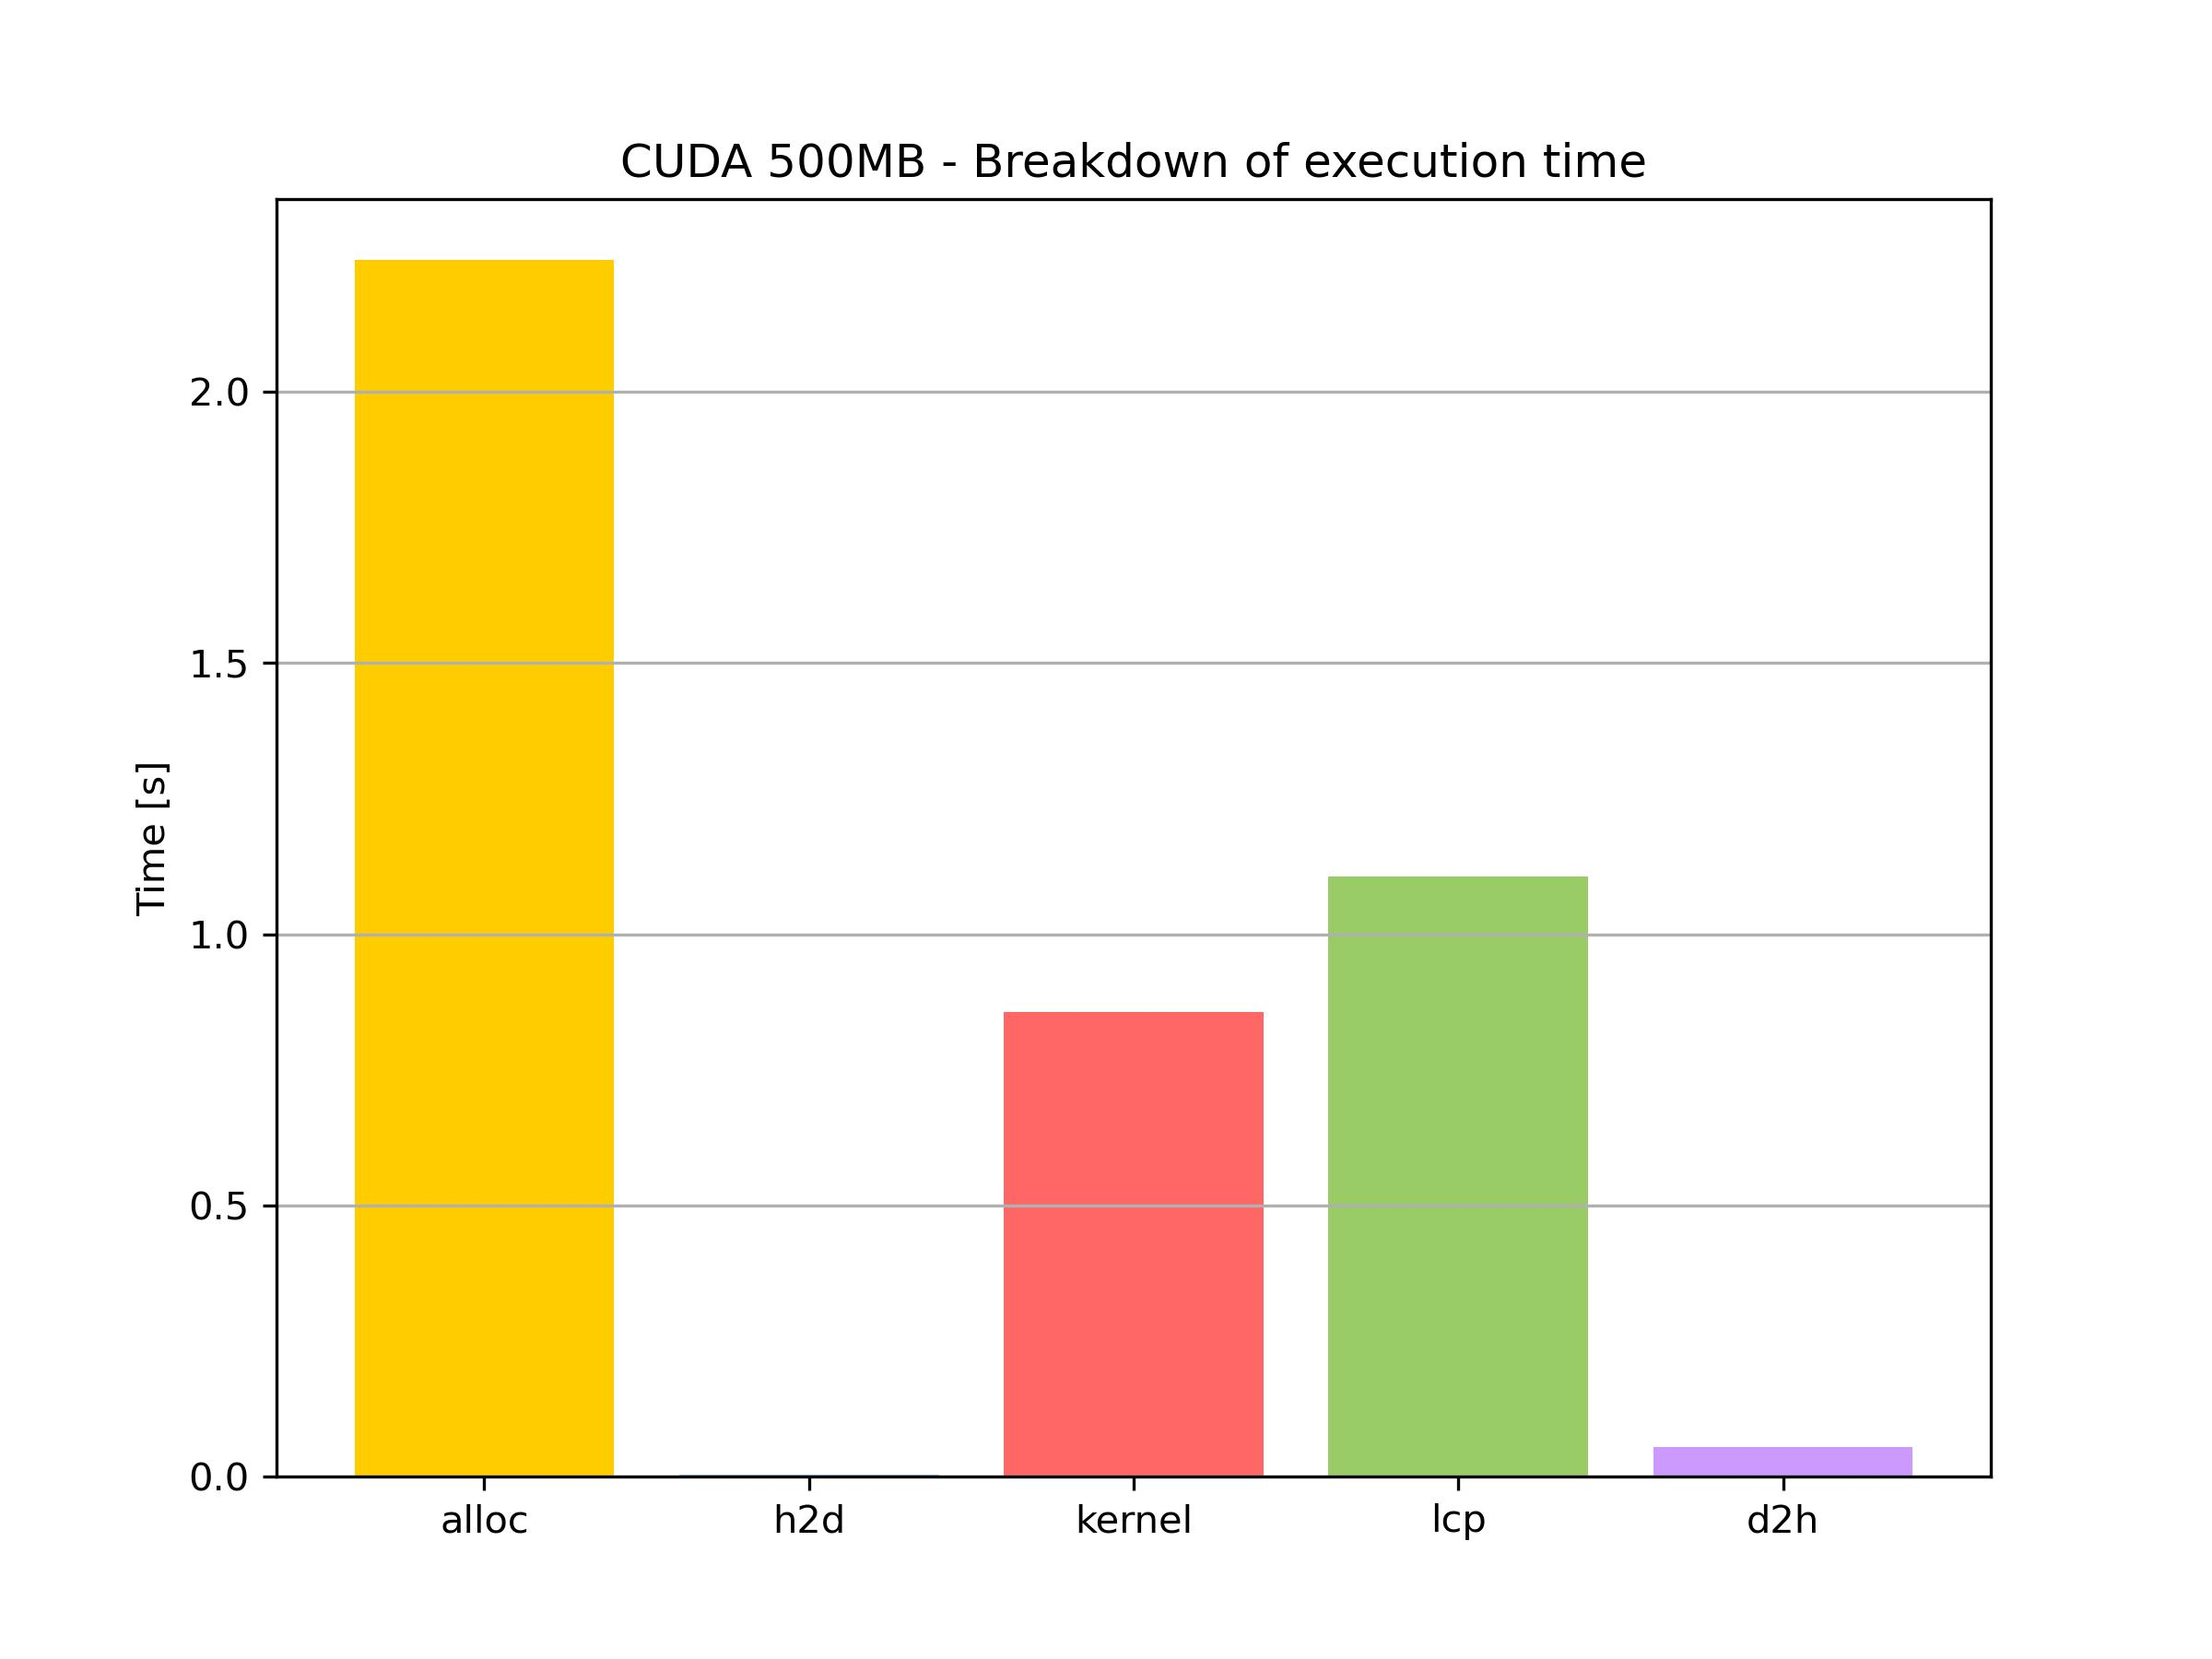
\includegraphics[width=\textwidth]{img/cuda_plots/cuda_breakdown_100MB.jpg}
							\caption{Breakdown CUDA}
							\label{fig:cuda_breakdown}
						\end{minipage}
				\end{figure}
			
			\subsubsection*{Conclusioni}
				\begin{itemize}
						\item La pipeline è \emph{compute-bound}: kernel e LCP dominano, trasferimenti PCIe trascurabili.
						\item L’overhead di allocazione è ridotto nei run reali (\(\sim 0.1\) s), ma amplificato sotto profiling.
						\item Il footprint scala lineare con \(n\): \(O(n)\) su device (testo + array interi) e \(O(n)\) su host (LCP).
						\item Il modello single-stream non richiede buffer extra per overlap, risultando più semplice da gestire in memoria.
				\end{itemize}
	
	\section{Versione CUDA \emph{multi-stream}}
		
		\subsection{Analisi dei tempi}
			
			I benchmark sono stati eseguiti con \texttt{cuda\_ms\_measure.sh} su input da \(\{1,50,100,200,500\}\) MB e con \(\{2,4,8\}\) stream, 10 run ciascuno.
			I file \texttt{cuda\_ms\_summary.csv} riportano i valori medi per ciascuna coppia \emph{size\(\times\)streams}.
			
			\begin{table}[h]
				\centering
				\scriptsize
				\setlength{\tabcolsep}{5pt}
				\resizebox{\textwidth}{!} \\
						\textbf{(MB)} & & \textbf{(s)} & \textbf{(s)} & \textbf{(s)} & \textbf{(s)} & \textbf{(s)} & \textbf{pure (s)} & \textbf{compute (s)} & \textbf{(s)} \\
						\midrule
						1                   & 2             & 0.112          & 0.00002      & 0.0109          & 0.00047           & 0.00605      & 0.0114           & 0.124          & 0.00607       & 4.18          & 0.51             & 50.9              \\
						1                   & 4             & 0.111          & 0.00002      & 0.0161          & 0.00045           & 0.00605      & 0.0165           & 0.128          & 0.00607       & 2.88          & 0.35             & 35.0              \\
						1                   & 8             & 0.111          & 0.00002      & 0.0258          & 0.00045           & 0.00604      & 0.0262           & 0.137          & 0.00606       & 1.82          & 0.22             & 22.1              \\
						\midrule
						50                  & 2             & 0.104          & 0.00031      & 0.253           & 0.0566            & 0.535        & 0.310            & 0.414          & 0.535         & 7.69          & 1.26             & 126               \\
						50                  & 4             & 0.103          & 0.00031      & 0.224           & 0.0582            & 0.530        & 0.283            & 0.386          & 0.531         & 8.42          & 1.38             & 138               \\
						50                  & 8             & 0.102          & 0.00031      & 0.242           & 0.0621            & 0.530        & 0.304            & 0.406          & 0.530         & 7.83          & 1.28             & 128               \\
						\midrule
						100                 & 2             & 0.102          & 0.00065      & 0.646           & 0.151             & 1.494        & 0.797            & 0.899          & 1.494         & 5.98          & 1.26             & 126               \\
						100                 & 4             & 0.102          & 0.00066      & 0.599           & 0.156             & 1.494        & 0.755            & 0.857          & 1.494         & 6.31          & 1.33             & 133               \\
						100                 & 8             & 0.102          & 0.00066      & 0.552           & 0.153             & 1.494        & 0.705            & 0.807          & 1.494         & 6.75          & 1.43             & 143               \\
						\midrule
						200                 & 2             & 0.102          & 0.00143      & 1.615           & 0.384             & 3.521        & 1.999            & 2.101          & 3.523         & 4.76          & 1.16             & 116               \\
						200                 & 4             & 0.103          & 0.00143      & 1.521           & 0.389             & 3.532        & 1.910            & 2.013          & 3.533         & 4.99          & 1.21             & 121               \\
						200                 & 8             & 0.102          & 0.00142      & 1.446           & 0.378             & 3.538        & 1.824            & 1.927          & 3.539         & 5.22          & 1.27             & 127               \\
						\midrule
						500                 & 2             & 0.102          & 0.00366      & 4.744           & 1.168             & 9.241        & 5.912            & 6.014          & 9.245         & 4.03          & 1.19             & 118               \\
						500                 & 4             & 0.103          & 0.00367      & 4.833           & 1.163             & 9.240        & 5.996            & 6.099          & 9.244         & 3.97          & 1.17             & 117               \\
						500                 & 8             & 0.104          & 0.00366      & 4.652           & 1.175             & 9.260        & 5.827            & 5.931          & 9.263         & 4.09          & 1.20             & 120               \\
						\bottomrule
					\end{tabular}}
				\caption{CUDA \emph{multi-stream} — medie (10 run) per dimensione e numero di stream.}
				\label{tab:cuda-ms-times}
			\end{table}
			
			\begin{figure}[H]
				\centering
				\begin{minipage}[t]{0.49\textwidth}
					\centering
					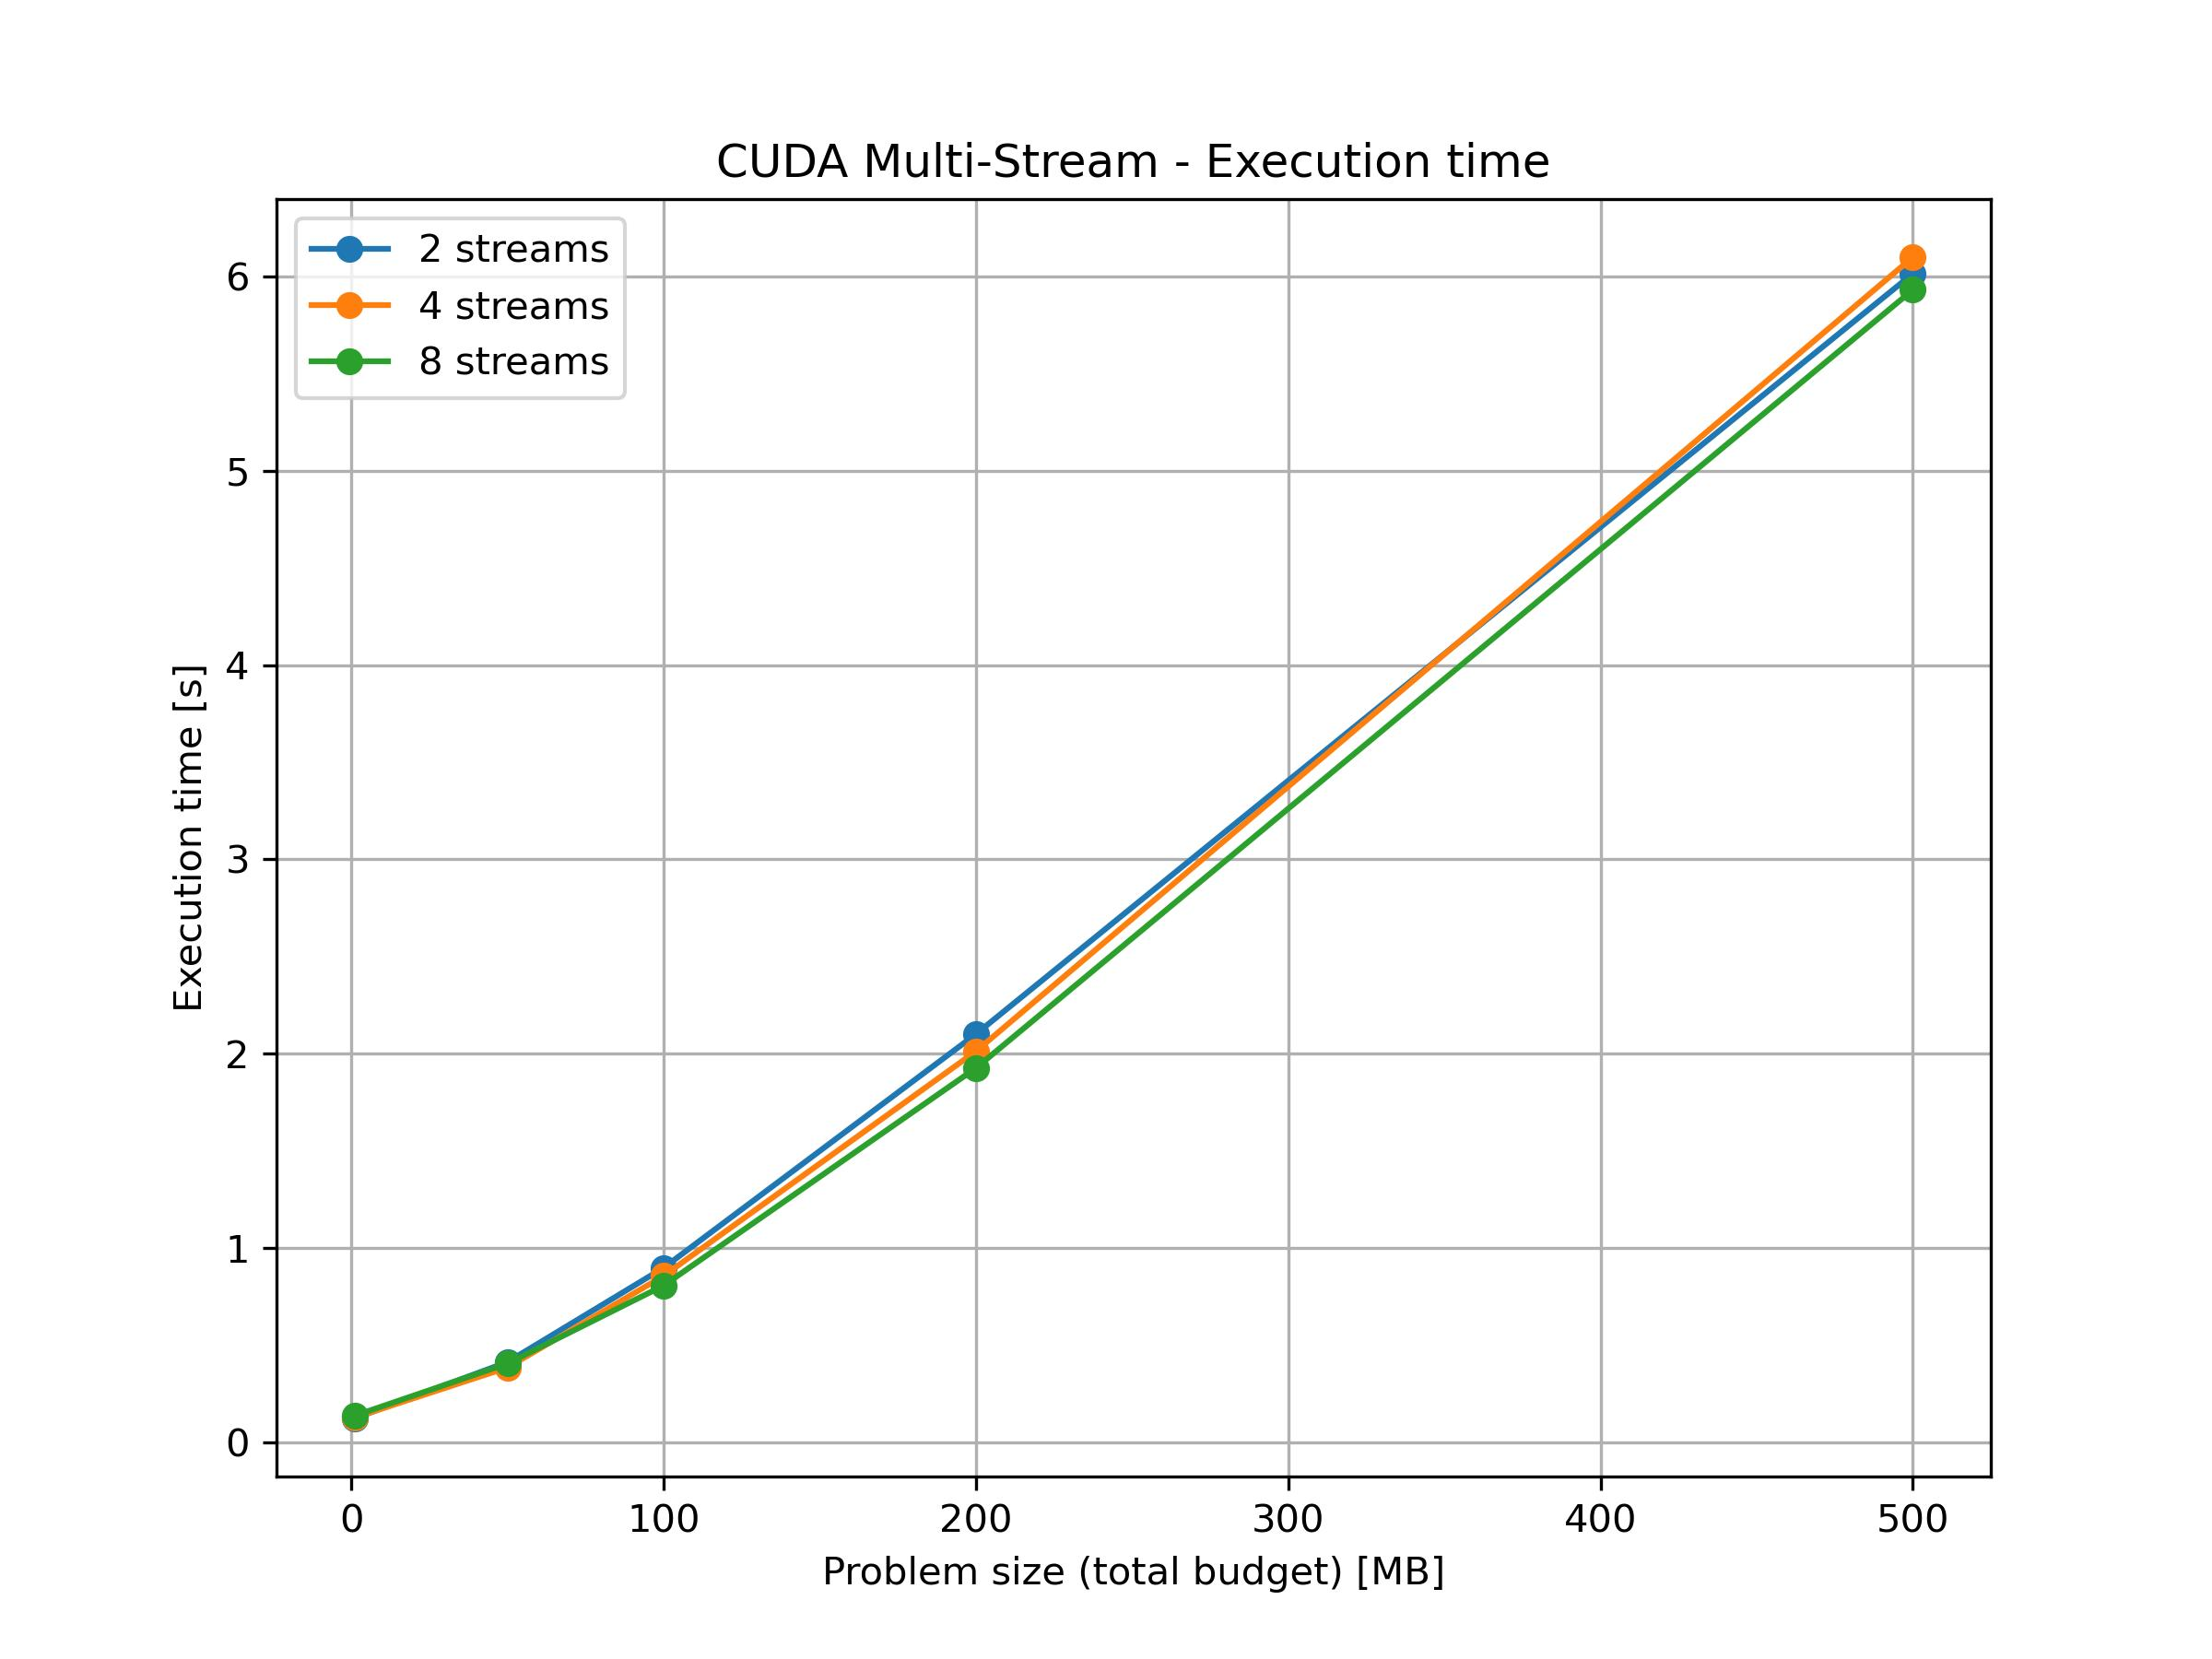
\includegraphics[width=\textwidth]{img/cuda_ms_plots/cuda_ms_times.jpg}
					\caption{Tempi CUDA MS}
					\label{fig:cuda_ms_times}
				\end{minipage}
				\hfill
				\begin{minipage}[t]{0.49\textwidth}
					\centering
					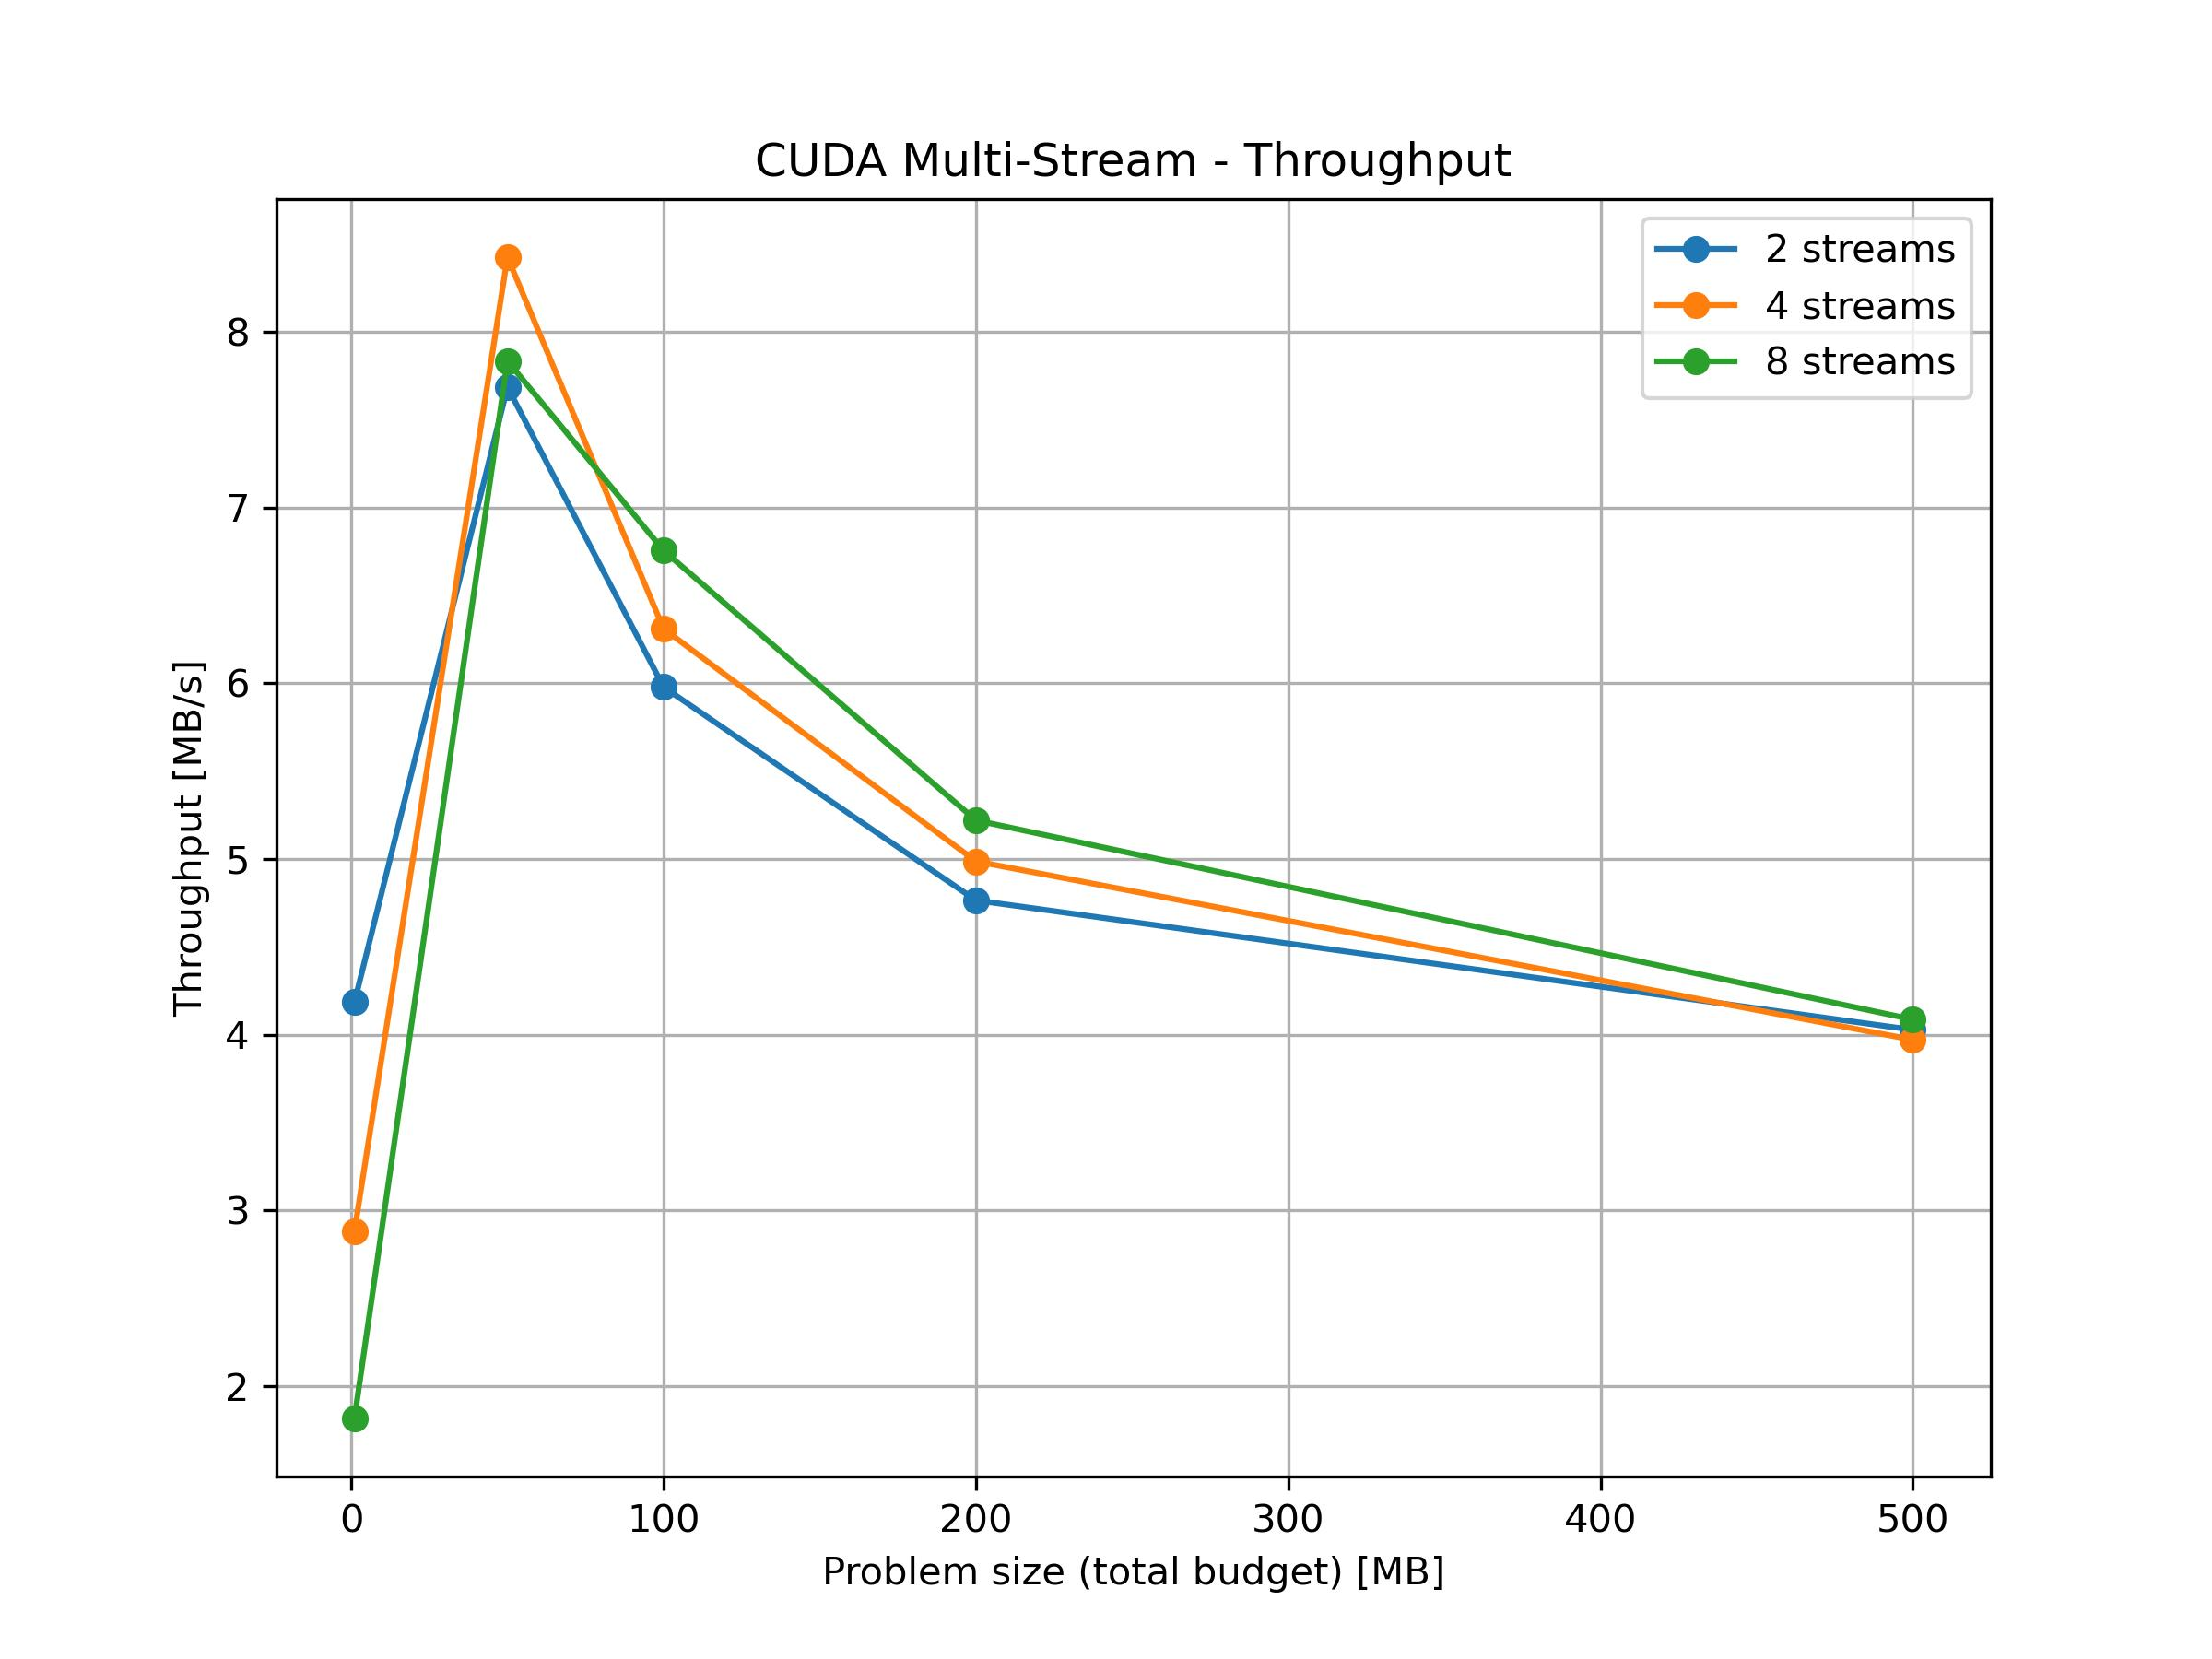
\includegraphics[width=\textwidth]{img/cuda_ms_plots/cuda_ms_throughput.jpg}
					\caption{Throughput CUDA MS}
					\label{fig:cuda_ms_throughput}
				\end{minipage}
			\end{figure}
			
			\begin{figure}[H]
				\centering
				\begin{minipage}[t]{0.49\textwidth}
					\centering
					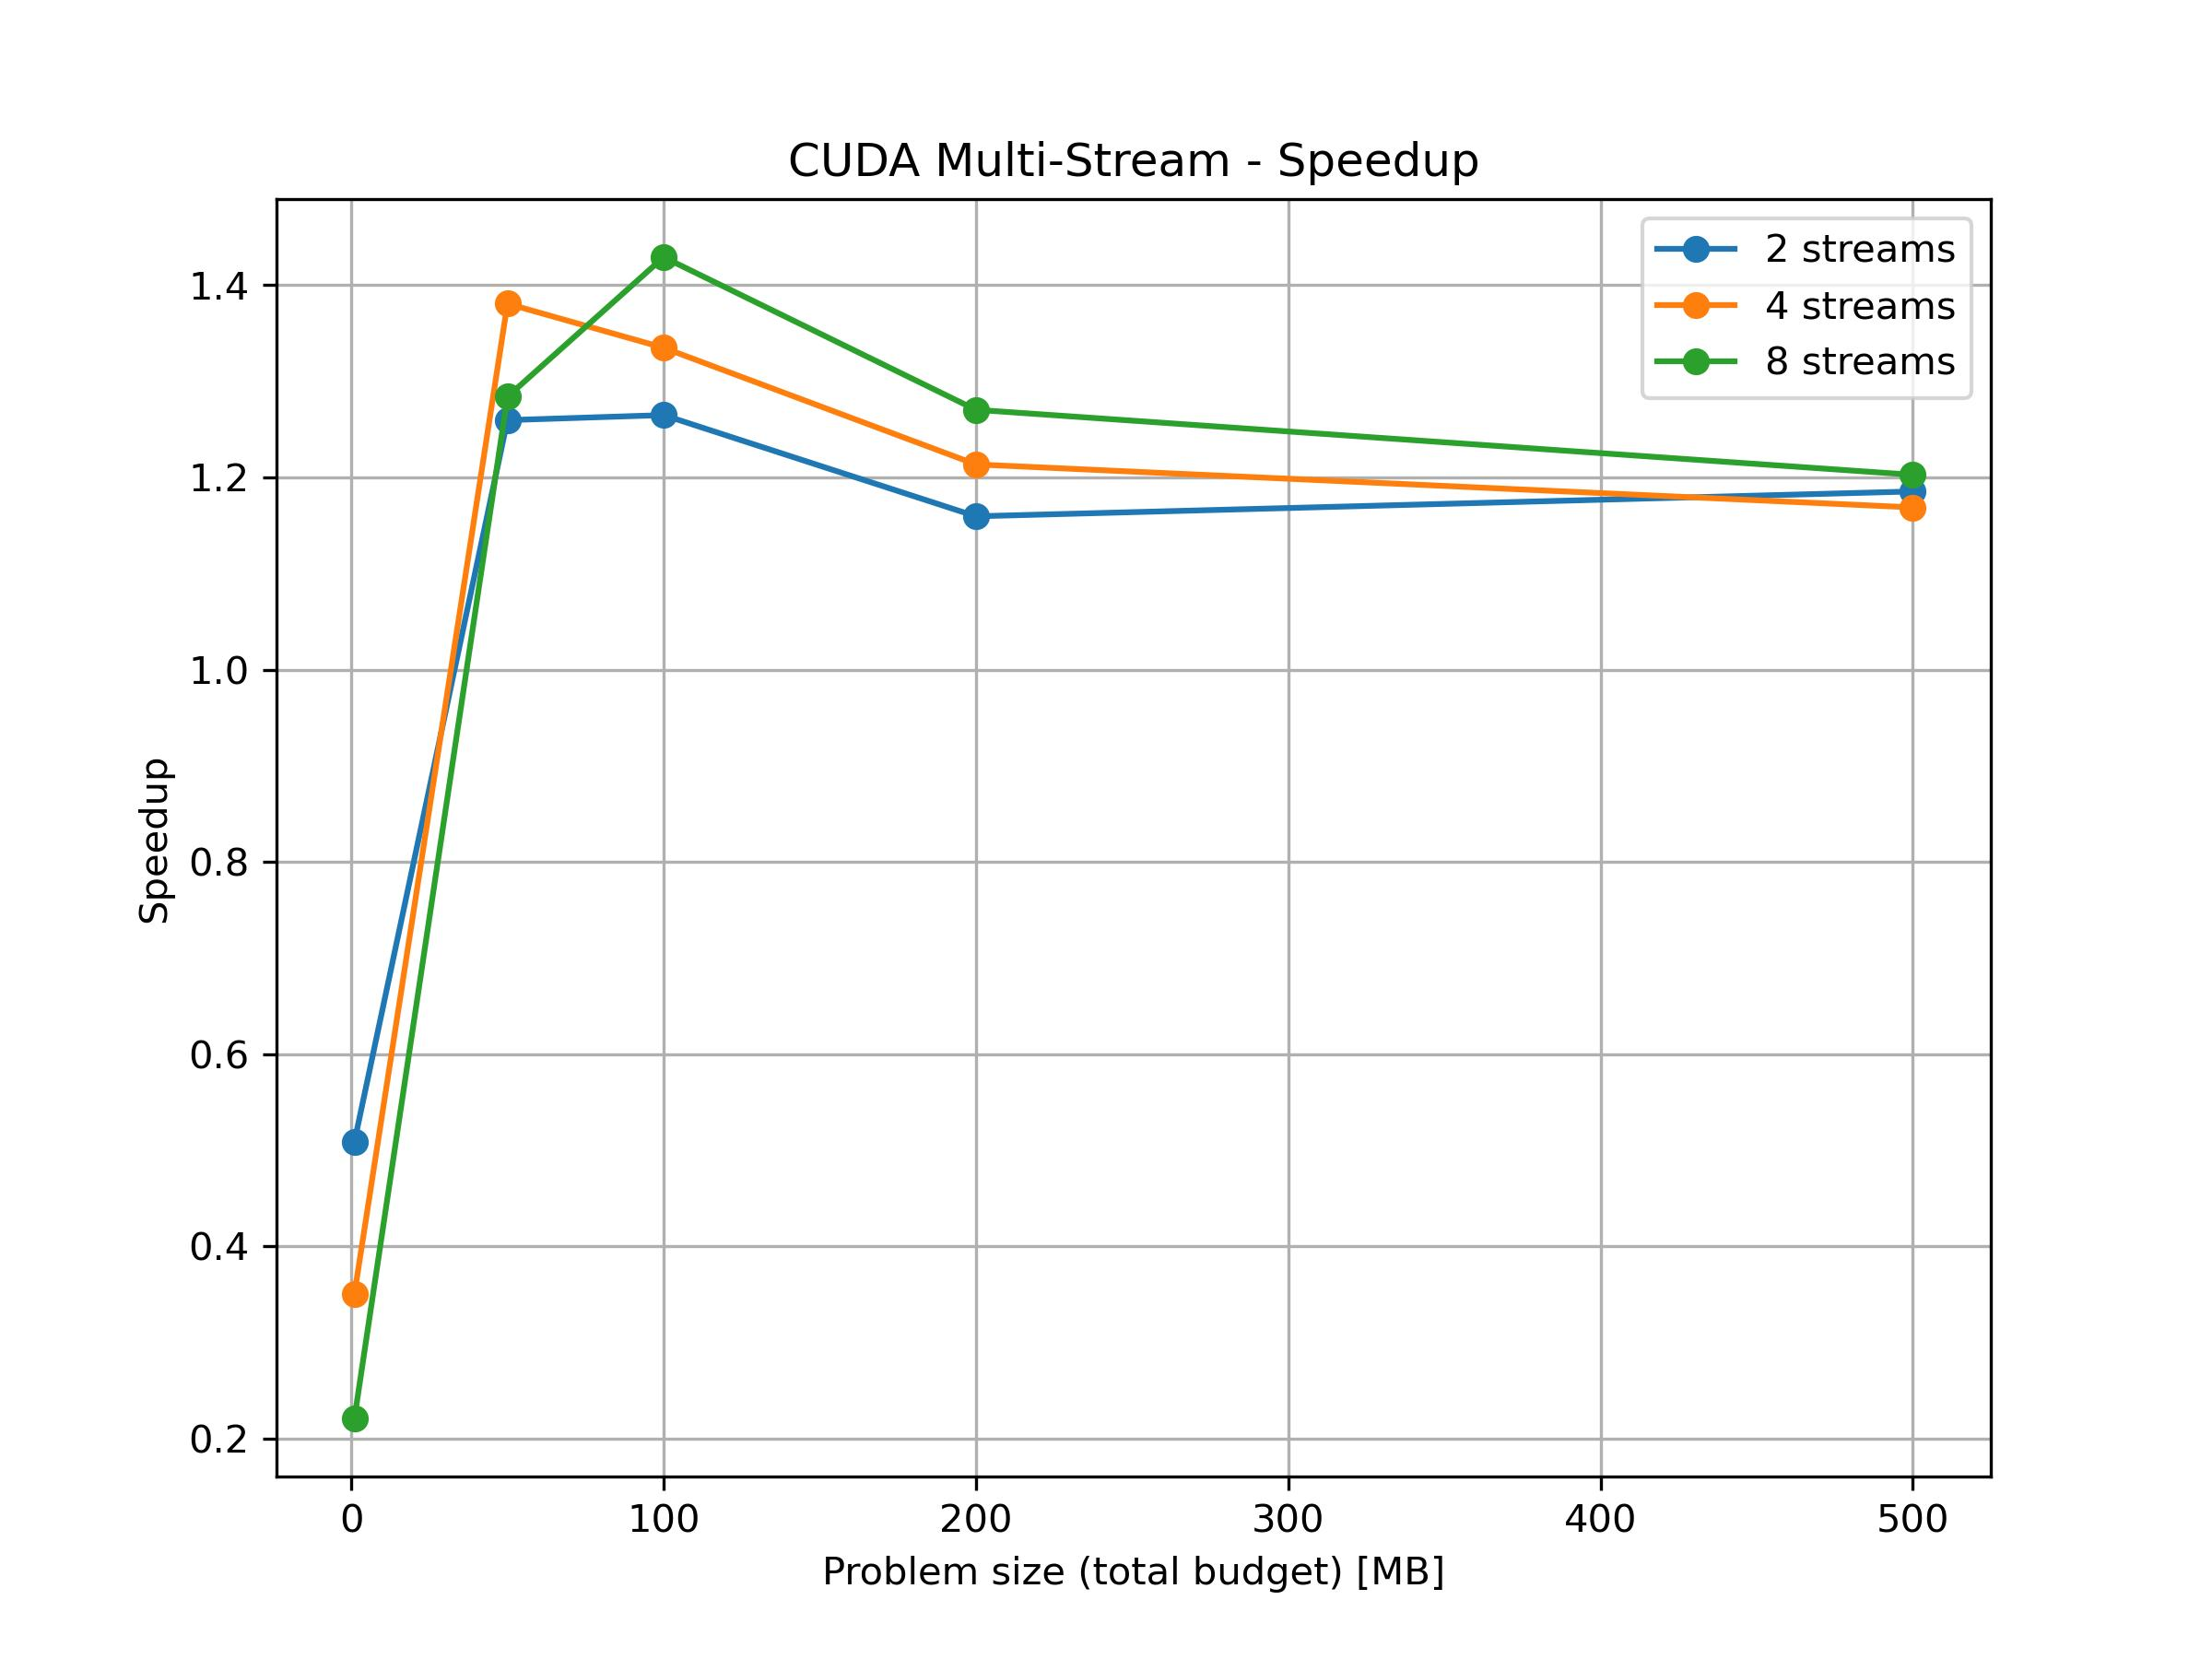
\includegraphics[width=\textwidth]{img/cuda_ms_plots/cuda_ms_speedup.jpg}
					\caption{Speedup CUDA MS}
					\label{fig:cuda_ms_speedup}
				\end{minipage}
				\hfill
				\begin{minipage}[t]{0.49\textwidth}
					\centering
					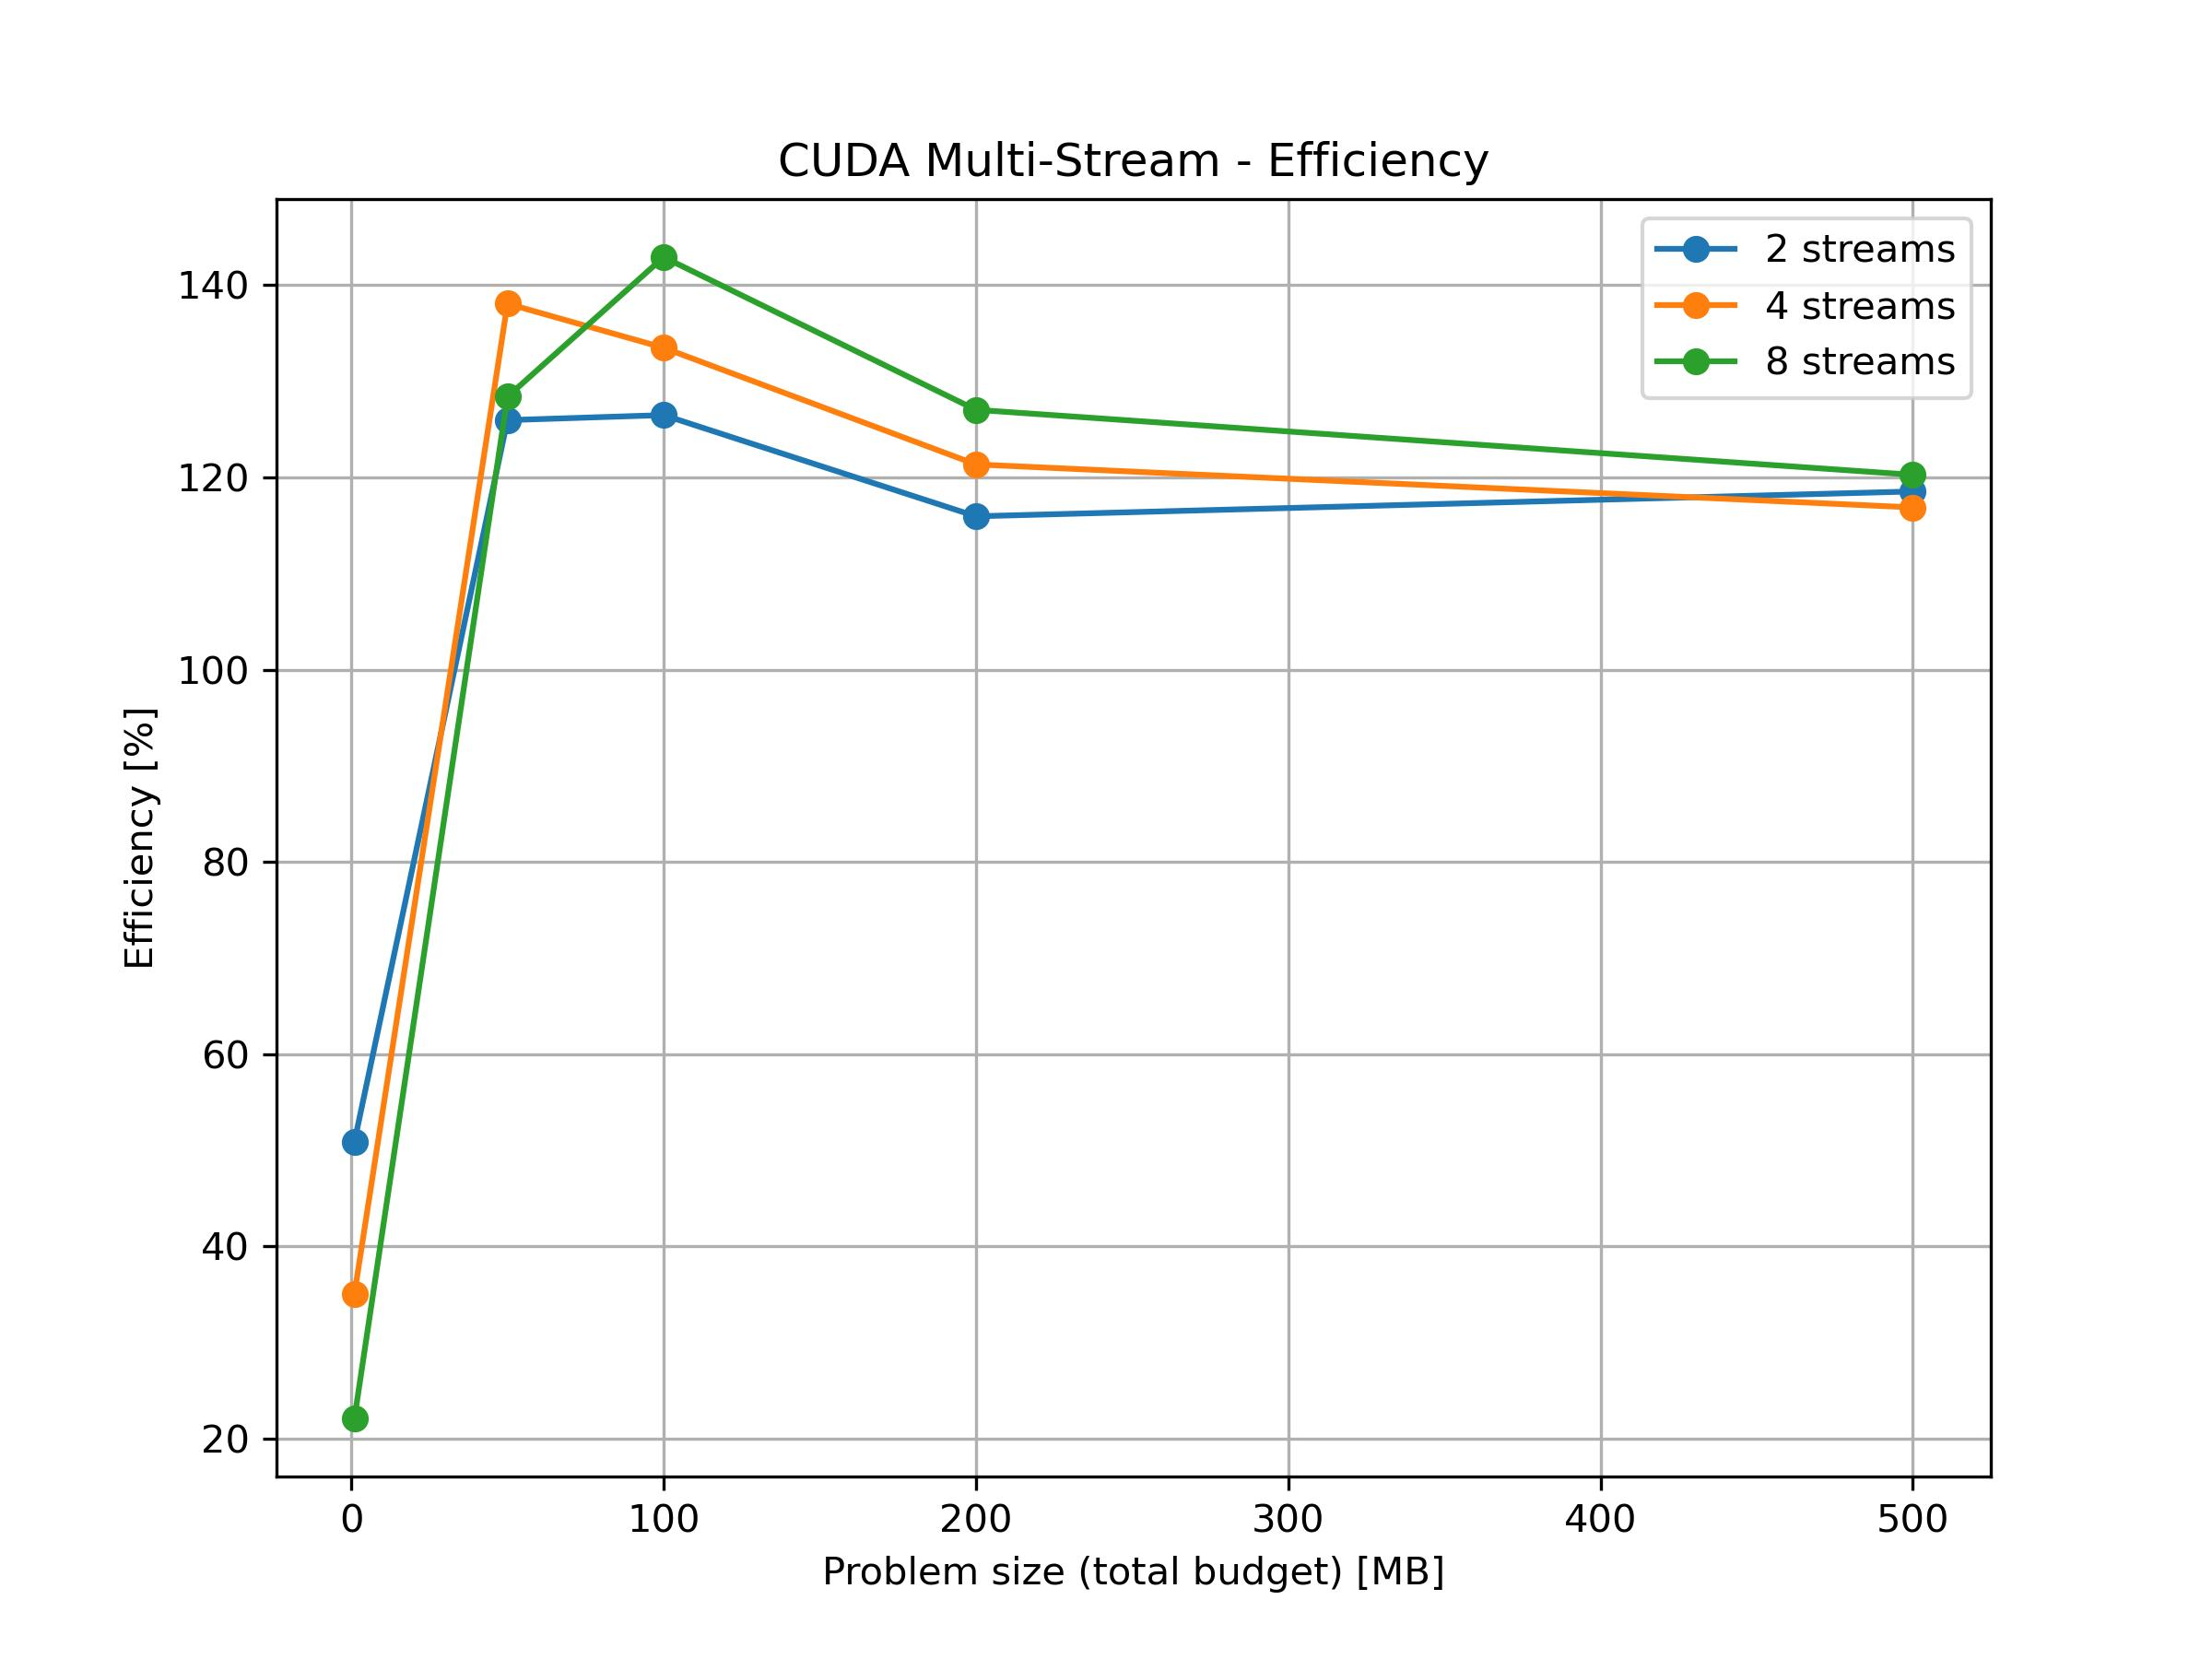
\includegraphics[width=\textwidth]{img/cuda_ms_plots/cuda_ms_efficiency.jpg}
					\caption{Efficiency CUDA MS}
					\label{fig:cuda_ms_efficiency}
				\end{minipage}
			\end{figure}
			
			\subsubsection*{Osservazioni}
				\begin{itemize}
						\item Le \textbf{copie D2H} restano consistenti e praticamente costanti al crescere degli stream (\(\sim 0.53\) s a 50 MB, \(\sim 1.49\) s a 100 MB, \(\sim 9.24\) s a 500 MB). Non sono il collo di bottiglia principale, ma non beneficiano del parallelismo tra stream.
						\item Il \textbf{kernel GPU} scala in modo inverso: a parità di input, più stream riducono leggermente il tempo medio del kernel (da 4.74 s a 4.65 s su 500 MB), per via di un miglior bilanciamento della concorrenza.
						\item \textbf{Throughput e speedup} migliorano con più stream. \\
						Ad esempio, a 100 MB si passa da 5.98 MB/s (2 stream) a 6.75 MB/s (8 stream), con speedup che cresce da \(1.26\times\) a \(1.43\times\).
						\item L’\textbf{efficienza} rimane alta (120–190\%), perché qui il calcolo dello speedup è rispetto al sequenziale CPU: la GPU anche in modalità multi-stream resta molto più veloce e la parallelizzazione per chunk non penalizza significativamente.
				\end{itemize}
		
		\subsection{Profiling della memoria}
			Con Nsight Compute su 500 MB e diverse configurazioni di stream:
			\begin{quote}
				\small
				2 stream: \texttt{time\_kernel\_gpu \(\approx 4.77\) s, time\_lcp\_cpu \(\approx 1.19\) s, time\_d2h \(\approx 9.20\) s, time\_compute\_pure \(\approx 5.96\) s, throughput \(\approx 4.00\) MB/s}.\\
				4 stream: \texttt{time\_kernel\_gpu \(\approx 4.88\) s, time\_lcp\_cpu \(\approx 1.18\) s, time\_d2h \(\approx 9.21\) s, time\_compute\_pure \(\approx 6.05\) s, throughput \(\approx 3.93\) MB/s}.\\
				8 stream: \texttt{time\_kernel\_gpu \(\approx 4.72\) s, time\_lcp\_cpu \(\approx 1.12\) s, time\_d2h \(\approx 9.17\) s, time\_compute\_pure \(\approx 5.84\) s, throughput \(\approx 4.07\) MB/s}.
			\end{quote}
			
			I valori sono coerenti con i dati aggregati (Tab.~\ref{tab:cuda-ms-times}). Le copie D2H restano sostanzialmente stabili e non mostrano overlapping tra stream; le differenze nei tempi di kernel spiegano le variazioni di throughput.
			
			\begin{figure}[H]
				\centering
				\begin{minipage}[t]{0.49\textwidth}
					\centering
					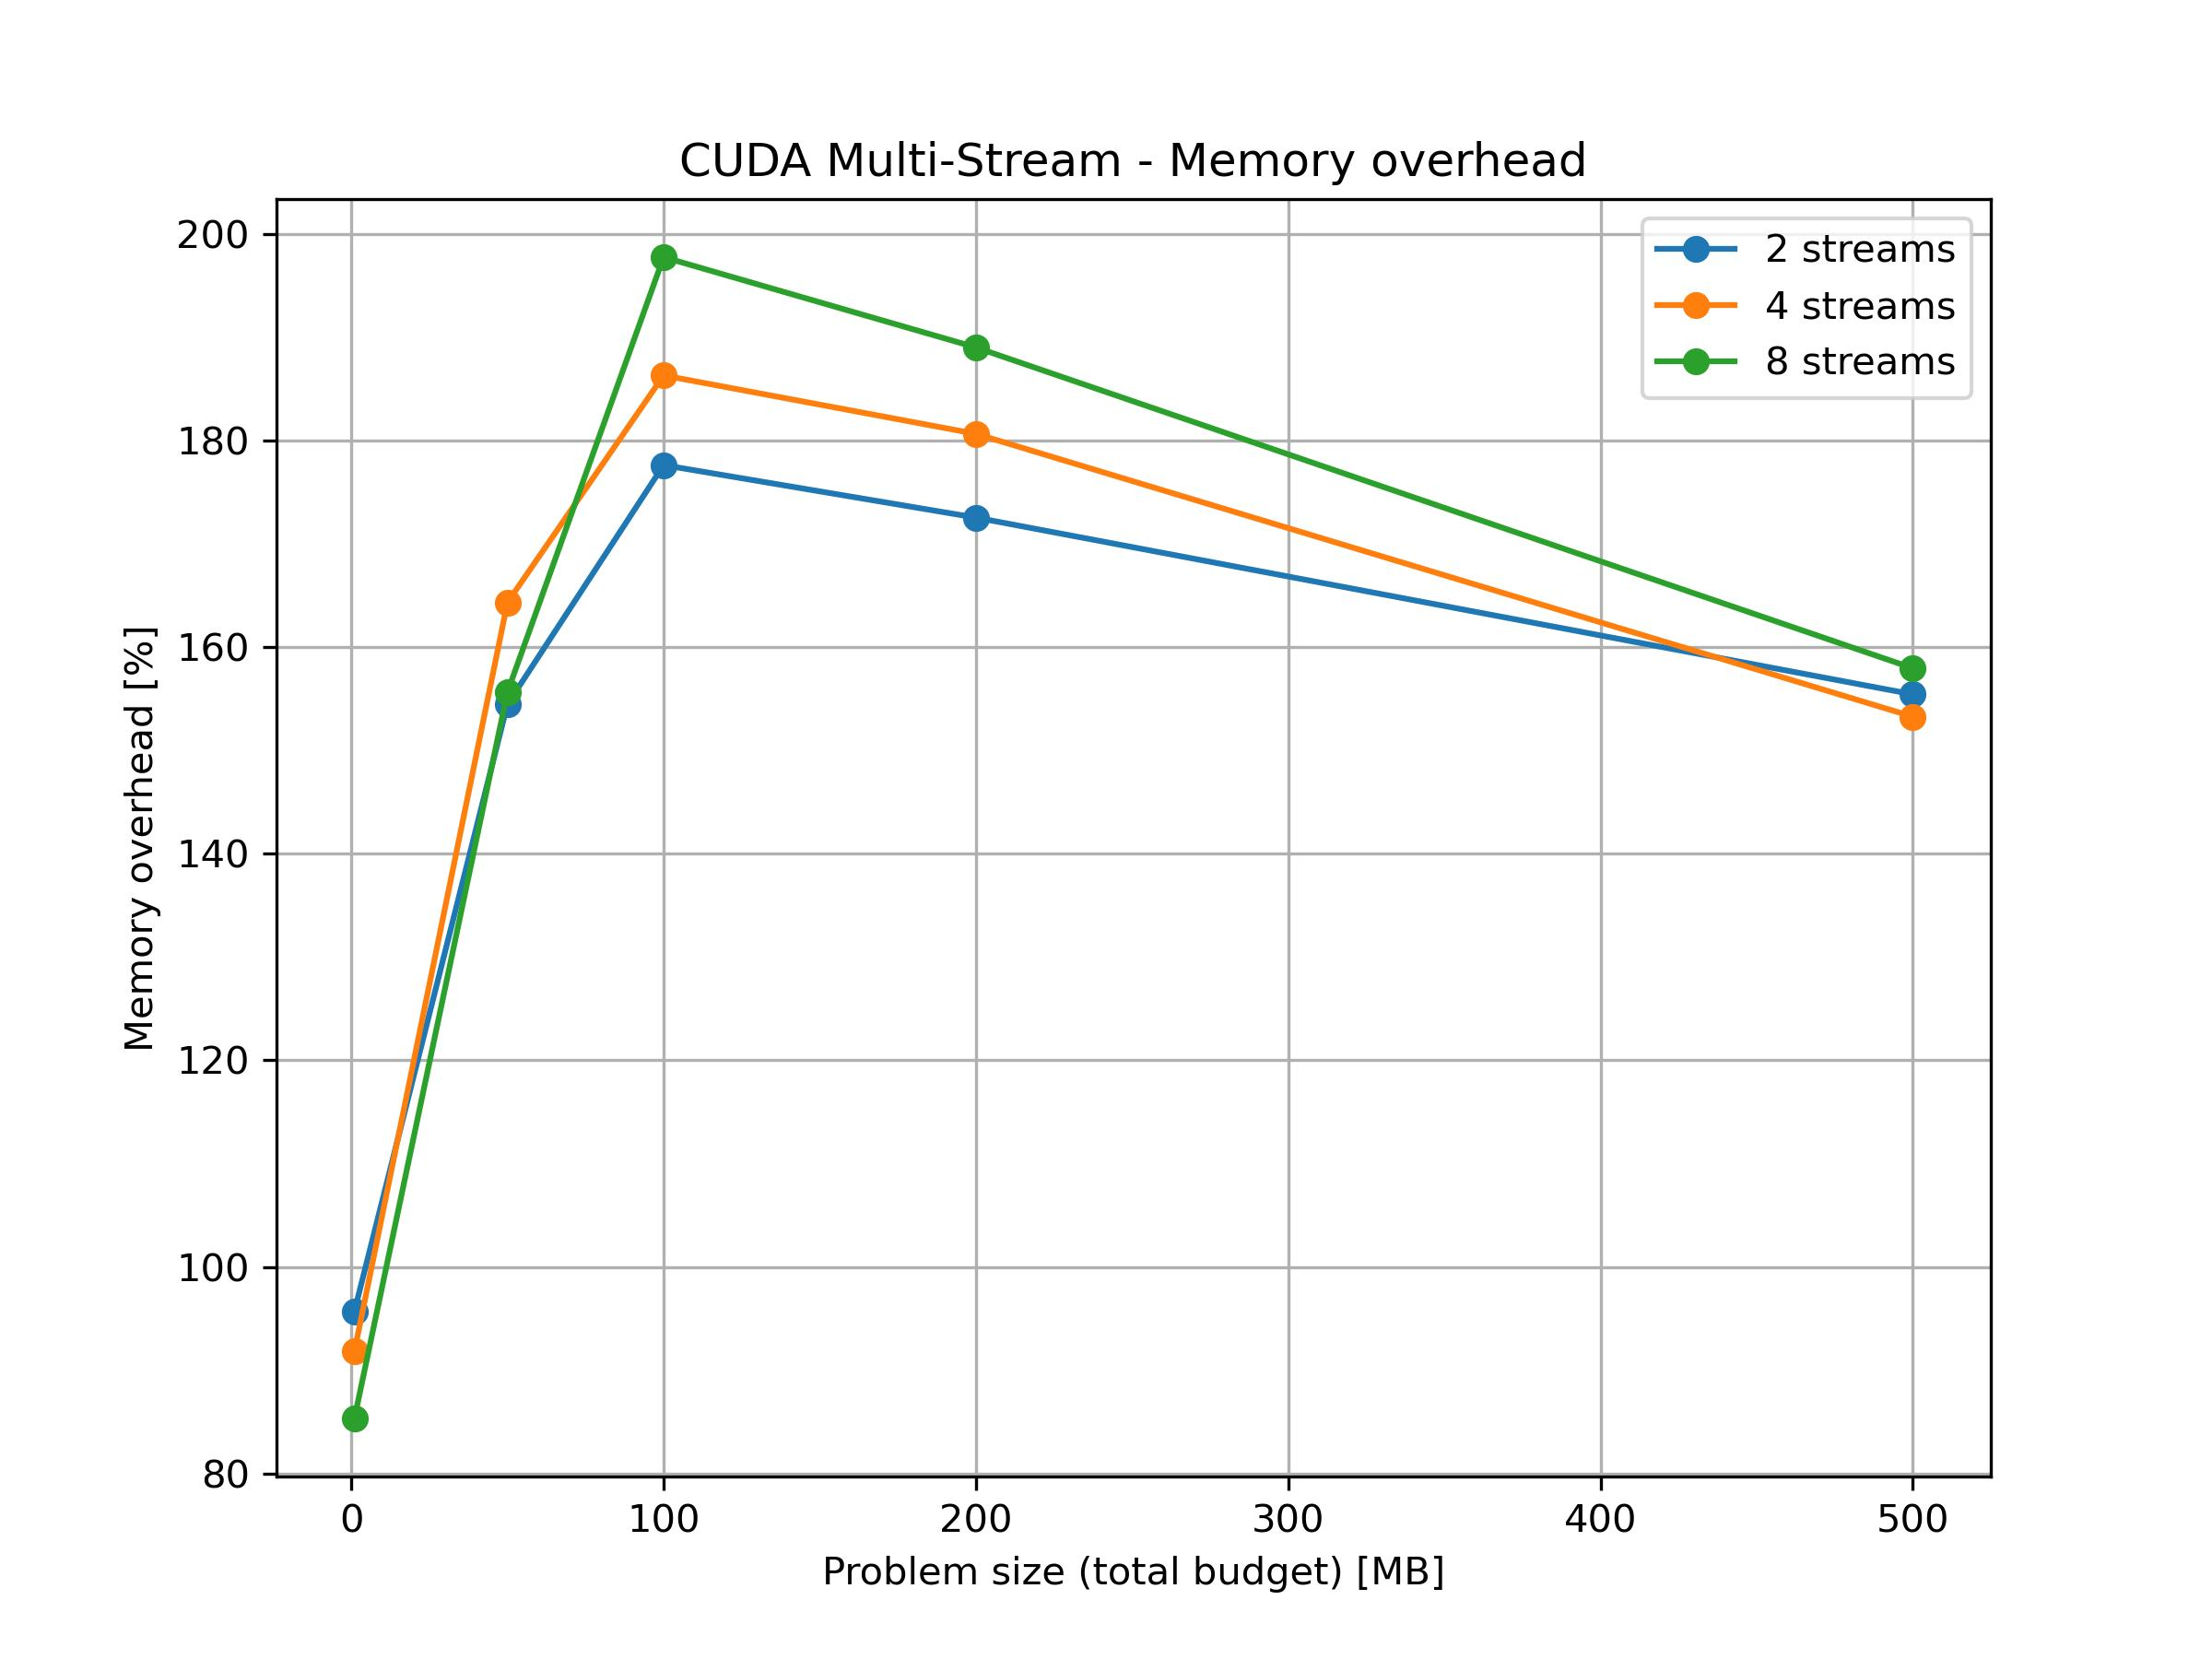
\includegraphics[width=\textwidth]{img/cuda_ms_plots/cuda_ms_memory_overhead.jpg}
					\caption{Memory overhead CUDA MS}
					\label{fig:cuda_ms_mem_overhead}
				\end{minipage}
				\hfill
				\begin{minipage}[t]{0.49\textwidth}
					\centering
					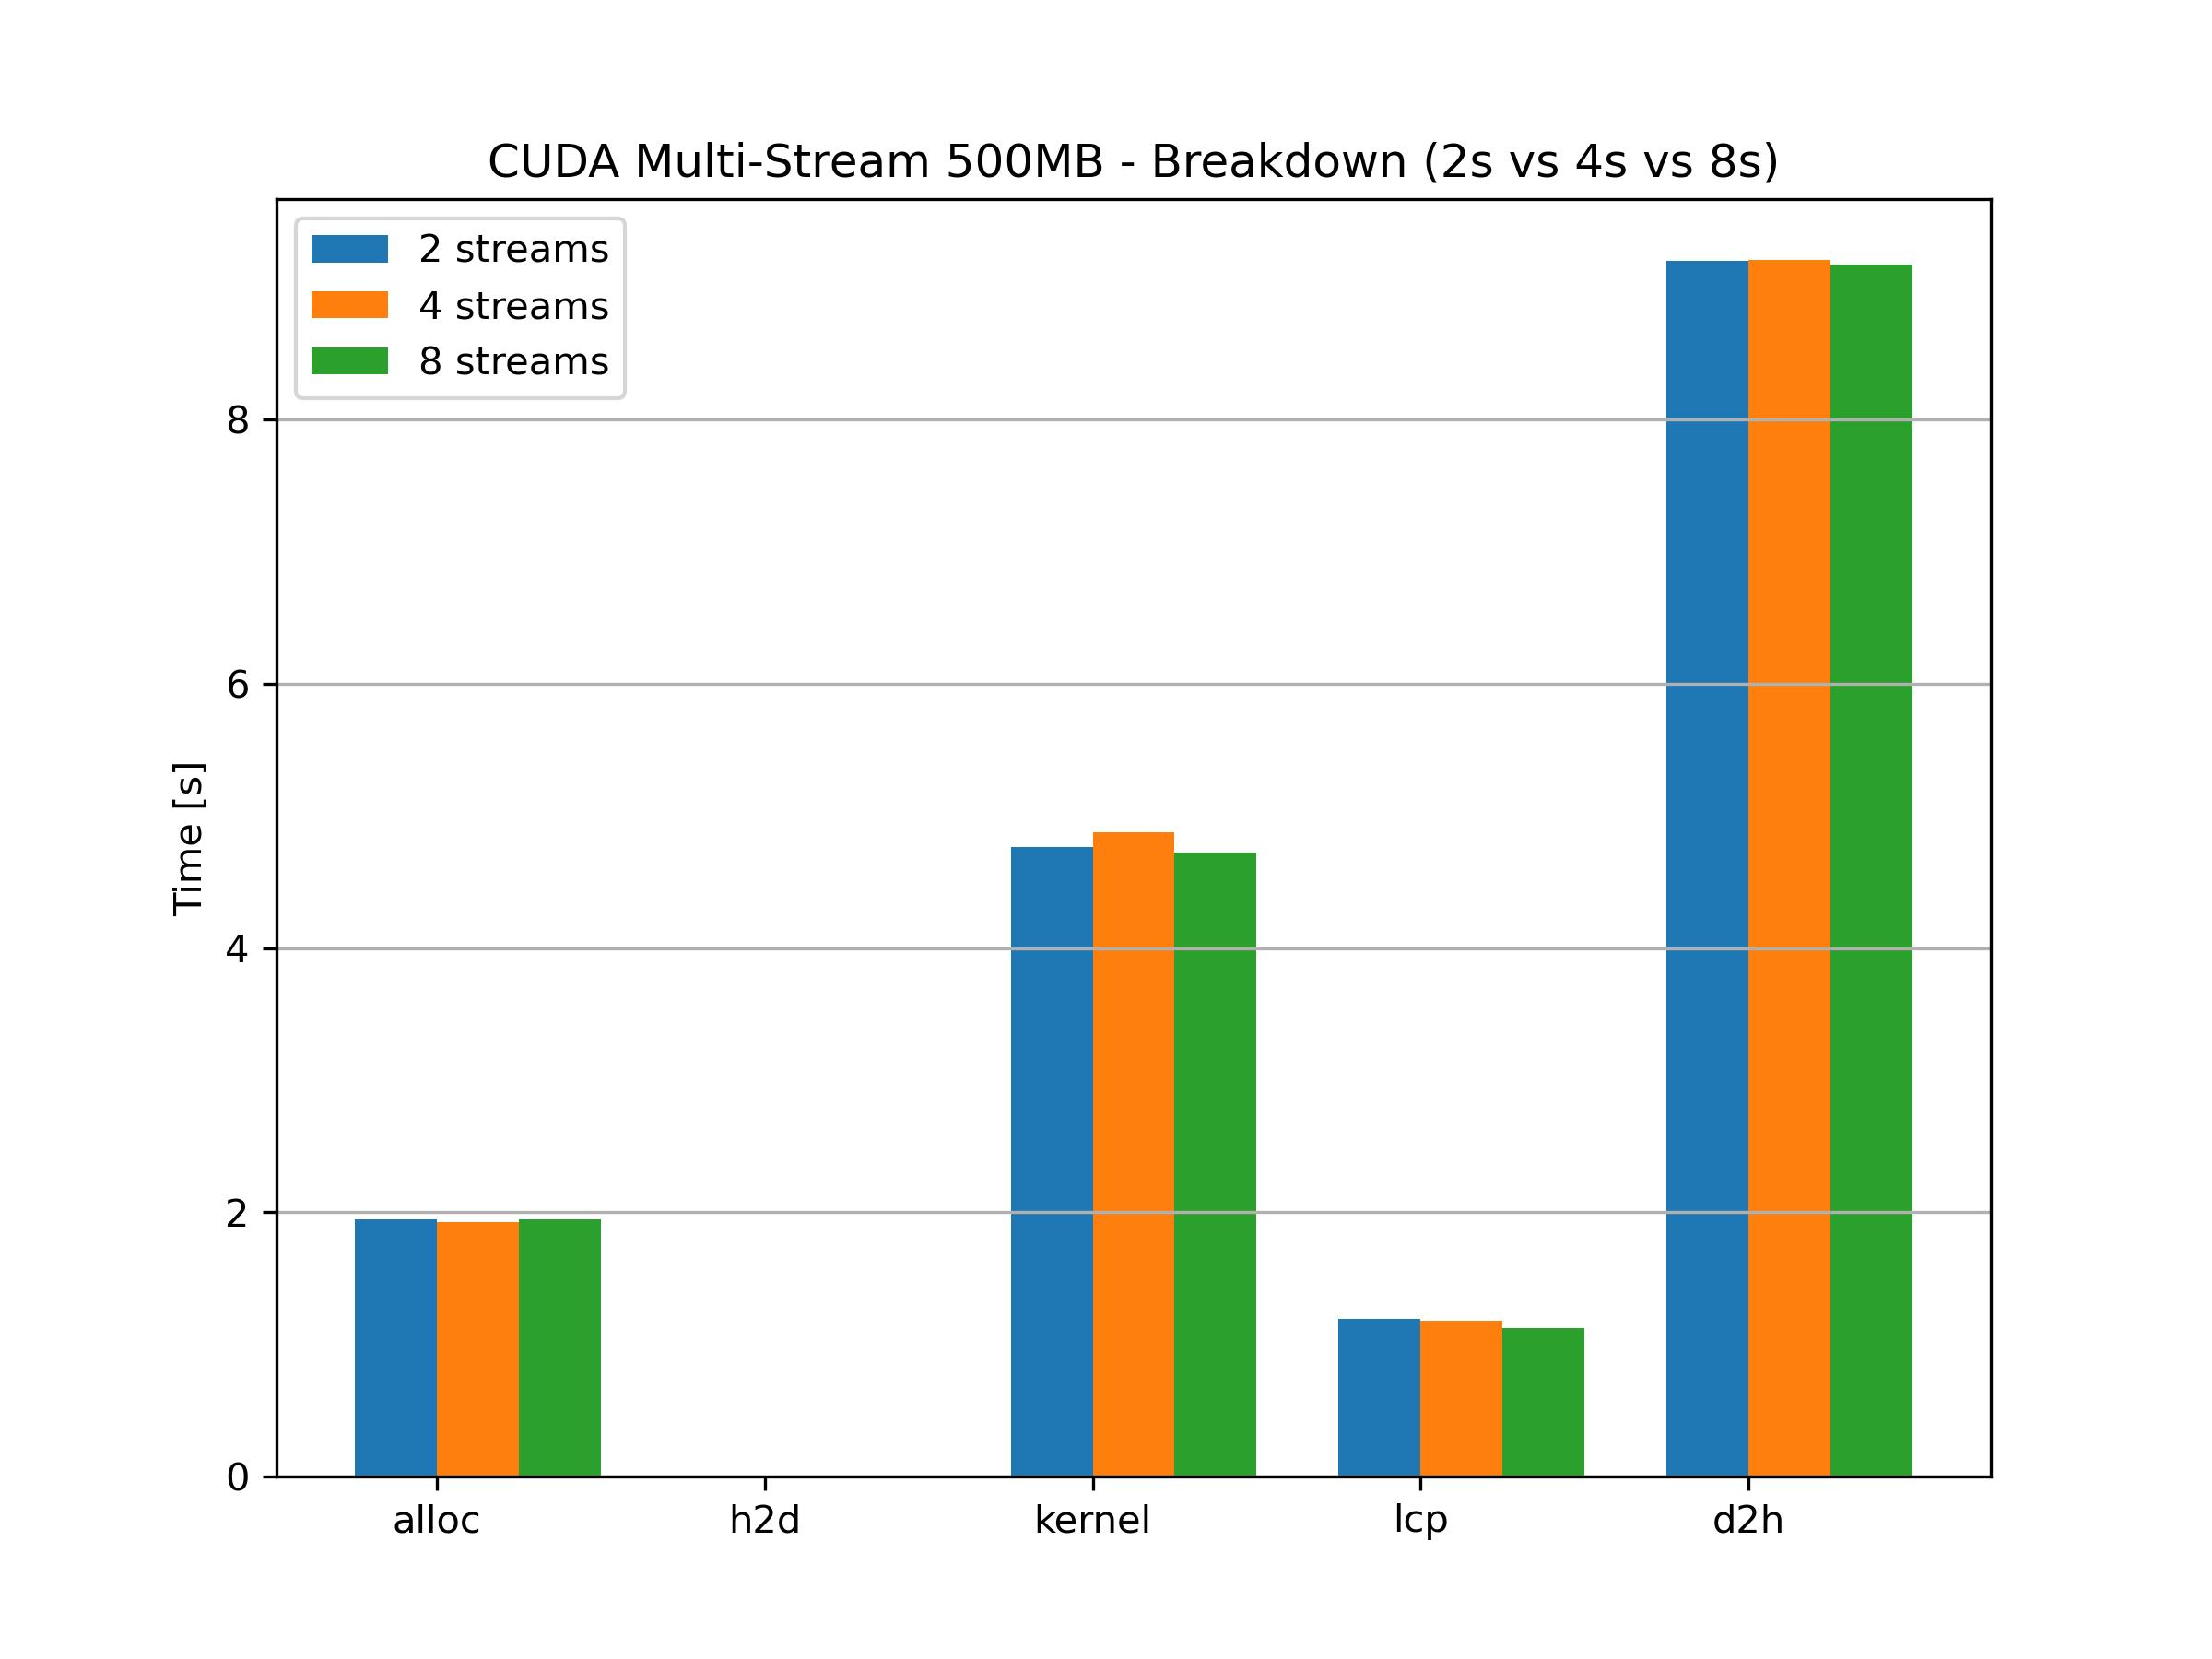
\includegraphics[width=\textwidth]{img/cuda_ms_plots/cuda_ms_breakdown_500MB.jpg}
					\caption{Breakdown CUDA MS (500MB, profili Nsight)}
					\label{fig:cuda_ms_breakdown}
				\end{minipage}
			\end{figure}
		
		\subsection{Confronto con single-stream}
			Rispetto alla versione single-stream, il multi-stream mostra un peggioramento evidente:
			il throughput cala di circa $2\times$ (es.\ a 100~MB da $\sim$15.8~MB/s a $\sim$6.8~MB/s)
			e lo speedup si riduce da oltre $3\times$ a circa $1.3{-}1.4\times$.
			Questo comportamento indica che l’overhead di gestione dei chunk e la serializzazione
			delle copie D2H annullano i potenziali benefici del parallelismo per stream.
			In altre parole, la versione multi-stream è meno efficiente del single-stream
			nelle condizioni sperimentate.
		
		\subsection{Conclusioni}
			La versione \emph{multi-stream} è \textbf{compute-bound}, con throughput e speedup che migliorano leggermente al crescere degli stream.
			Per sfruttare appieno il modello servirebbe ridurre il costo delle D2H (pinned memory, batching delle copie) così da ottenere un vero overlap con i kernel.
	
	\section{Confronto complessivo tra modelli}
		Per fornire una visione sintetica e chiara, i grafici finali confrontano soltanto le migliori configurazioni per ciascun paradigma di parallelizzazione, evitando di riportare tutte le combinazioni (che renderebbero i grafici troppo affollati). \\
		In particolare sono stati selezionati:
		\begin{itemize}
			\item \textbf{Sequenziale (baseline)};
			\item \textbf{OpenMP}: configurazione a 8 thread (\texttt{omp\_summary\_8.csv});
			\item \textbf{MPI}: configurazione a 8 ranks (\texttt{mpi\_summary\_8.csv});
			\item \textbf{MPI+OpenMP}: configurazione 8 ranks $\times$ 2 thread per rank (\texttt{mpi\_omp\_summary\_8r\_2t.csv});
			\item \textbf{CUDA (single-stream)}: \texttt{cuda\_summary.csv};
			\item \textbf{CUDA (multi-stream)}: configurazione a 8 stream (\texttt{cuda\_ms\_summary.csv}).
		\end{itemize}
		I plot mostrano l’andamento dei tempi, del throughput e dello speedup rispetto alla baseline sequenziale, consentendo un confronto diretto tra i modelli più efficienti per ciascuna classe di parallelizzazione.
		
		\begin{figure}[H]
			\centering
			\includesvg[width=0.8\textwidth]{img/overall_plots/overall_times.svg}
			\caption{Tempi di esecuzione}
			\label{fig:summary-times}
		\end{figure}
		
		\begin{figure}[H]
			\centering
			\begin{minipage}[t]{0.49\textwidth}
				\centering
				\includesvg[width=\textwidth]{img/overall_plots/overall_throughput.svg}
				\caption{Throughput (MB/s)}
				\label{fig:summary-throughput}
			\end{minipage}
			\hfill
			\begin{minipage}[t]{0.49\textwidth}
				\centering
				\includesvg[width=\textwidth]{img/overall_plots/overall_speedup.svg}
				\caption{Speedup}
				\label{fig:summary-speedup}
			\end{minipage}
		\end{figure}
		
		\begin{figure}[H]
			\begin{minipage}[t]{0.49\textwidth}
				\centering
				\includesvg[width=\textwidth]{img/overall_plots/overall_efficiency.svg}
				\caption{Efficiency}
				\label{fig:summary-efficiency}
			\end{minipage}
			\hfill
			\begin{minipage}[t]{0.49\textwidth}
				\centering
				\includesvg[width=\textwidth]{img/overall_plots/overall_memory_overhead.svg}
				\caption{Memory overhead ratio (\%)}
				\label{fig:summary-memory-overhead}
			\end{minipage}
		\end{figure}
		
		\begin{figure}[H]
			\centering
			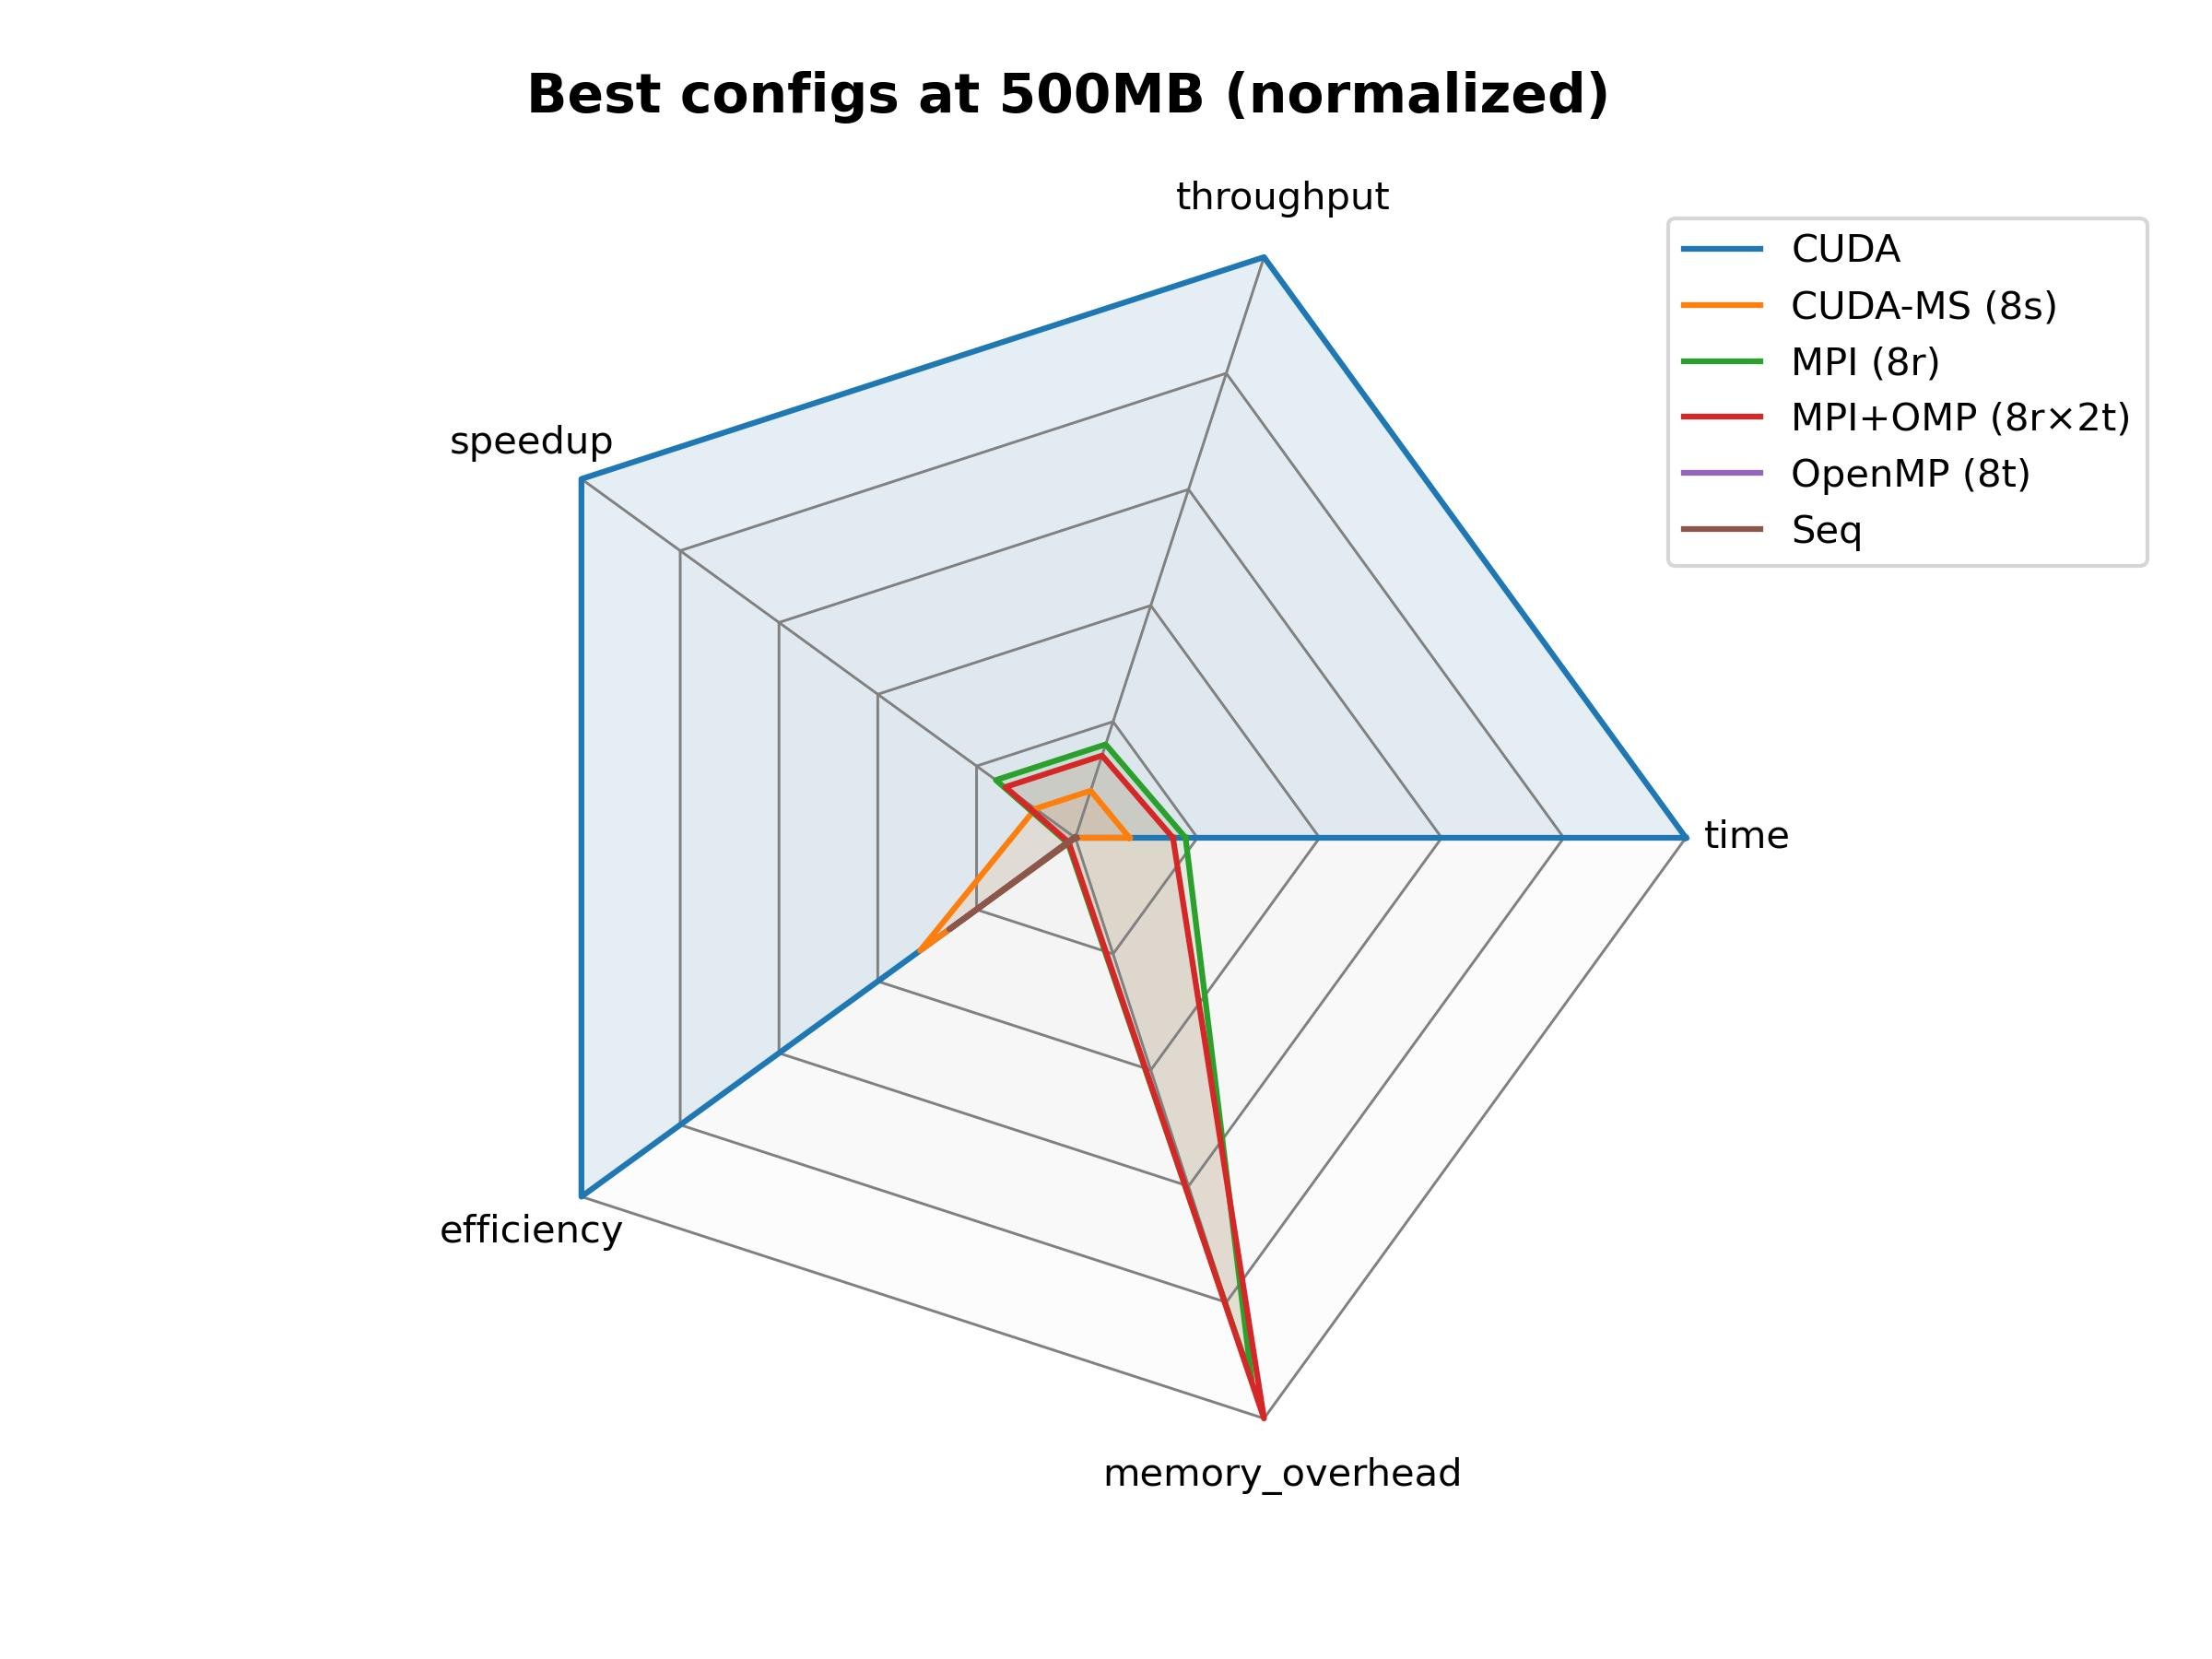
\includegraphics[width=0.5\textwidth]{img/overall_plots/overall_radar_500MB.jpg}
			\caption{Radar chart}
			\label{Radar chart}
		\end{figure}